\documentclass[oneside,a4paper]{book}
\usepackage{sty/packages}
\usepackage{sty/macros}
\usepackage{pretext/titlepage}  % Set header style

\begin{document}

	% A hack so numbering don't appear in parts, toc and intro
	% \pagestyle{empty}
	% \fancypagestyle{plain}{%
	% 	\fancyhf{}                          % clear all header and footer fields
	% 	\renewcommand{\headrulewidth}{0pt}
	% 	\renewcommand{\footrulewidth}{0pt}
	% 	\addtocounter{\thepage}{1}
	% }


	% Renew the plain style
\fancypagestyle{plain}{%
	\fancyhf{}                          % clear all header and footer fields
	\renewcommand{\headrulewidth}{0pt}
	\renewcommand{\footrulewidth}{0pt}
	% \addtocounter{\thepage}{1}
}  % Renew the plain page style 
	\pagestyle{plain}

	% \frontmatter	
	\newgeometry{top=5cm,bottom=3cm,left=3cm,right=3cm}
		\maketitle
	\restoregeometry
	% % \title{[Sem título]}
% \author{Carlos Augusto Belini de Gois}
% %\date{}
% %
% \begin{titlingpage}
% 	\maketitle
% 	\begin{center}
% 	\begin{minipage}{.7\textwidth}
% 		\centering Dissertação de mestrado submetida ao Programa de Pós-Graduação em Física do Instituto de Física \enquote{Gleb Wataghin} da Universidade Estadual de Campinas para título de mestre.
% 	\end{minipage}
% 	\end{center}
	
% 	\vfill
% 	\begin{center}
% 	\begin{minipage}{.7\textwidth}
% 		\centering Departamento de Física da Matéria Condensada\\Instituto de Física \enquote{Gleb Wataghin}\\Universidade Estadual de Campinas
% 	\end{minipage}
% 	\end{center}
% 	\vspace{3.5em}
% \end{titlingpage}

\title{Classicality and dense coding in the prepare-and-measure scenario}
\author{Carlos Augusto Belini de Gois}
\def\advisor{Prof. Dr. Rafael Luiz da Silva Rabelo}           
\def\university{Universidade estadual de Campinas} 

%%%%%%%%%%%%%%%%%%%%%%%
% Formatação da capa
%%%%%%%%%%%%%%%%%%%%%%%

\renewcommand{\maketitle}[1][]{%
 \begin{titlepage}
   %\OnehalfSpacing
   %\let\footnotesize\small \let\footnoterule\relax 
   \vskip-\headsep
   \begin{center}
     {\Large\textbf{ \@title }\par}
     \vspace{3em}
     {\large \@author}\par
     \vspace{1em}
     Supervisor:\\
     {\large \advisor}\par
	 {\vfill}
     \MakeUppercase{\university}
   \end{center}
   \vspace*{.5in}
 \end{titlepage}
}%

	\newgeometry{top=5cm,bottom=5cm,left=8cm,right=3cm}
		\clearpage
\begin{center}
    \thispagestyle{empty}
    \vspace*{\fill}
    \begin{displayquote}[Thomas Pynchon --- Mason \& Dixon]
    	\emph{The Telescope, the Fluxions, the invention of Logarithms and the frenzy of multiplication, often for its own sake, that follow’d have for Emerson all been steps of an unarguable approach to God, a growing clarity,--- Gravity, the Pulse of Time, the finite speed of Light present themselves to him as aspects of God’s character. It’s like becoming friendly with an erratic, powerful, potentially dangerous member of the Aristocracy. He holds no quarrel with the Creator’s sovereignty, but is repeatedly appall’d at the lapses in Attention, the flaws in Design, the squand’rings of life and energy, the failures to be reasonable, or to exercise common sense,--- first appall’d, then angry. We are taught,--- we believe,--- that it is love of the Creation which drives the Philosopher in his Studies. Emerson is driven, rather, by a passionate Resentment.}
    \end{displayquote}
    \vspace*{\fill}
\end{center}
\clearpage
	\restoregeometry
	\begingroup
\let\clearpage\relax

\chapter*{Abstract}
\thispagestyle{empty}

AAAAAAAAAAAAAAA

\chapter*{Resumo}
\thispagestyle{empty}

BBBBBBBBBBBBBBB

\endgroup
	\chapter*{Publications}
% \addcontentsline{toc}{chapter}{Introduction}
\thispagestyle{empty}

	\begin{itemize}
		\item \bibentry{degois_2021_general}
		\item \bibentry{moreno_pamdense_2021}
	\end{itemize}
	\chapter*{Acknowledgments}
% \addcontentsline{toc}{chapter}{Introduction}
\thispagestyle{empty}

	\newgeometry{top=3cm,bottom=4cm,left=3cm,right=3cm}
		\tableofcontents
	\restoregeometry

	% \mainmatter

	\chapter*{Introduction}
\addcontentsline{toc}{chapter}{Introduction}
% \thispagestyle{empty}
\label{chap:introduction}

In the widest sense, \emph{quantum information} is the study of the encoding, processing, and decoding of information by means of quantum systems. The field came about during the '80s and '90s, when groundbreaking results in quantum computing \cite{feynman2018simulating,shor1999polynomial} and, most notably, quantum cryptography \cite{bb84,ekert91}, connected informational with foundational aspects of quantum theory. Ultimately, this paved the way that turned quantum information into a vast and thriving research field.

\emph{Correlation scenarios} are central to quantum information. In an important subset of correlation scenarios, two or more parties locally interact with and read out information from their respective systems. When only two parties are considered, it is usual to call them Alice and Bob and think of each as being in their own lab, locally interacting with their own experiments. It so happens that Alice's and Bob's results can be \emph{correlated}, even in cases where no communication takes place during the experiment. There is nothing surprising in observing correlations, after all, they commonly arise in all sorts of physical systems. However, something interesting happens if we further ask \emph{to what extent} correlations are present: when the underlying systems are assumed to go by the laws of classical physics, the possible correlations obey a certain structure that, strikingly, can sometimes be violated by quantum systems. This puts a clear divide between the behaviors of classical, quantum, and even more exotic systems \cite{prbox}. More than that, because such violations can be determined from measurement results alone, Alice and Bob can certify whether they are dealing with quantum systems even when they have no previous knowledge about their experiments. It is then usual to picture the systems as being inside black-boxes that can only be investigated by providing inputs (e.g., representing measurement choices) and collecting outputs. This is the so-called \emph{device-independent} paradigm, of which the most well-known example is that of Bell nonlocality \cite{brunner_2014_nonlocality}. %Remarkably, it is possible to show that nonlocal behaviors require \emph{entanglement} and \emph{measurement incompatibility}, which are two structures at the core of the most surprising phenomena described by quantum theory. %Therefore, observing them, more than showing us the devices must contain quantum systems, also tells us these systems must be entangled, and the measurements, albeit uncharacterized, have to be incompatible.
Nonlocal behaviors are also precisely the characteristic that allows for provably secure quantum key distribution protocols \cite{ekert91}, communication complexity \cite{buhrman_communicationreview_2010}, and many other informational applications of device-independent correlation scenarios \cite{brunner_2014_nonlocality}. From a more foundational perspective, stashing systems into black-boxes let us to hide implementation details, and thus examine classical, quantum, and other theories for themselves. The question of what, exactly, is \emph{quantum} in quantum theory has puzzled scientists for more than a century, and the device-independent paradigm is closely linked to modern investigations on this topic \cite{barrett_gpts_2007,plavala_gpts_2021,spekkens_2005_contextuality}.  

% Collecting the results obtained by each party, one can analyze whether they are independent or correlated. In the latter case, we can further ask \emph{to what extent} such correlations are present. When the underlying systems are assumed to be classical, these correlations obey certain bounds that, strikingly, can be violated by some quantum systems. This puts a clear divide between the behaviors of classical, quantum, and even more exotic systems \cite{prbox}. Because this distinction is observable from measurement results alone, correlation scenarios can be used to device-independently certify quantum behaviors. In the \emph{device independent} paradigm, each system is inside a black-box to which we impose no extra assumptions. All observations happen by providing inputs to the boxes and collecting their outputs. Even if no communication is allowed between the boxes, certain quantum systems are still certifiably so. Because of this no-signalling hypothesis, any correlation manifest between the systems must have been present from the start. Remarkably, it is possible to show that quantum behaviors in this so-called Bell nonlocality scenario require \emph{entanglement} and \emph{measurement incompatibility}, which are two structures at the core of the most surprising phenomena described by quantum theory. Thus, observing nonlocal behaviors, more than showing us the boxes must contain quantum systems, also tells us these systems must be entangled, and the measurements, albeit uncharacterized, have to be incompatible. Nonlocal behaviors are precisely the characteristic that allow for provably secure quantum key distribution protocols \cite{ekert91}, randomness certification, and many other informational applications of device independent correlation scenarios \cite{brunner_2014_nonlocality}. From a more foundational perspective, stashing systems into black boxes allow us to hide implementation details, and thus examine classical, quantum and other theories for themselves. The question of what, exactly, is \emph{quantum} in quantum theory has puzzled scientists for more than a century, and the device independent paradigm is closely linked to modern investigations on this topic \cite{barrett_gpts_2007,plavala_gpts_2021,spekkens_2005_contextuality}.

This thesis will be largely concerned with employing the device-independent paradigm to investigate quantum communication protocols, which are clever ways of encoding, transmitting, and subsequently decoding information using quantum systems. To be useful in practice, quantum communication must provide some kind of advantage over the common practice of using classical systems for similar tasks. This is exactly the case in the dense coding protocol \cite{bennett_1992_superdense}. In it, one party communicates a $d$-dimensional quantum system to another and, by exploiting pre-existing entanglement, the receiving end may perfectly recover two classical $d$its of information, thus doubling the capacity of a noiseless classical communication channel. This celebrated protocol is also remarkable for its theoretical simplicity, and its applicability paves the way towards the development of quantum technologies. However, dense coding has only been discussed in the device-\emph{dependent} case, where one has full knowledge on which states may be prepared and what measurements can be applied. To turn it device \emph{in}dependent, we must look for a correlation scenario with a causal structure that presupposes communication --- the aforementioned Bell nonlocality scenario does not. The simplest choice is the \emph{prepare and measure scenario}. In chap. \ref{chap:pam-quantum}, we will see how doing so leads to several entanglement witnesses, the possibility of self-testing maximally entangled states, and a procedure to search for which states or measurements lead to the best probability of success in the dense coding protocol.

The prepare and measure scenario (chap. \ref{chap:pam-classical}) has been attracting growing attention in recent years. Part of this interest comes from it being useful for quantum key distribution \cite{pawlowski_pamqkd_2011} and self-testing quantum systems \cite{tavakoli_selftesting_2018,tavakoli_selftesting_2020}, while they can also be seen as building blocks for quantum communication networks \cite{poderini_pamcriteria_2020,bowles_pamnetworks_2015}. In the simplest instance of a prepare and measure scenario (fig. \ref{fig:pam-scenario}), a preparation device receives an input, then prepares and communicates \emph{some} system to a measurement device which, given another input by a second observer, outputs a result. Calling our friends for help, we may picture Alice operating the preparation device, and Bob the measurement one. Many practical tasks in this scenario involve Alice wanting to send some message to Bob through a limited amount of communication, and in that case, we can see the preparation as the encoding, the communicated system as the carrier, and the measurement as the decoder of the message. Only observational data is collected by each of the two parties, which means the devices are black-boxes. Similar to how we can tell quantum from classical behaviors apart in Bell nonlocality scenarios, it is sometimes also possible to device independently certify that nonclassical communication happened in a prepare and measure experiment. As nonclassical behaviors are the ones that may lead to quantum advantages in communication, an important question arising in this context is whether some set $\mathcal{S}$ of possible quantum preparations can manifest nonclassical behaviors. Measurements play a crucial role in this regard. To necessarily and sufficiently certify the classicality of $\mathcal{S}$, one needs to test the preparations under all the infinitely many possible measurements. This is precisely the problem we tackle in chap. \ref{chap:pam-classical}, where we devise a general method to certify whether an arbitrary set of preparations always behaves in a way that classical systems also could. When this is the case, $\mathcal{S}$ is not useful for quantum enhancement in communication protocols. More than constructing the method, we also use it to prove the existence of a quantum advantage activation phenomenon in random access coding \cite{ambainis_qracsoriginal_1999}, another important communication protocol. In that same chapter, we turn the question inside-out by asking whether some set $\mathcal{M}$ of quantum \emph{measurements} is useful to reveal nonclassical behaviors. Quantum measurements differ from their classical counterparts in that they can be incompatible. Given that no entanglement is present in this instance of prepare and measure scenarios, incompatibility is a good candidate for the origin of quantum behaviors. Through the method built for this second task, we prove there are incompatible measurements that nevertheless cannot give rise to nonclassical behaviors, thence that incompatibility is not sufficient for nonclassicality in the prepare and measure scenario. %This is in stark contrast to quantum steering scenarios \cite{wiseman_2007_steering,uola_2020_steering,cavalcanti_2016_steering}, where incompatibility is necessary and sufficient for steerability \cite{quintino_incompatibilitysteering_2014,uola_onetoonesteering_2015}.



% An important relaxation on the nonlocality scenario is to allow for signalling between devices. These (semi-)device independent communication scenarios are attracting growing attention, as particularly in the case of \emph{prepare-and-measure} scenarios. Part of this interest is due to the fact that they are useful for quantum key distribution \cite{pawlowski_pamqkd_2011} and self-testing quantum systems \cite{tavakoli_selftesting_2018,tavakoli_selftesting_2020}, and can be seen as building blocks for quantum communication networks \cite{poderini_pamcriteria_2020,bowles_pamnetworks_2015}. In the simplest instance of a prepare-and-measure scenario, a preparation device receives an input, then prepares and communicates \emph{some} system to a measurement device which, given another input by a second observer, outputs a result. Again, only observational data is collected by each of the two parties, which may later be collectively analyzed. Similarly to how we can tell quantum from classical behaviors apart in nonlocality scenarios, it is sometimes also possible to device independently certify that quantum --- rather than classical ---, communication happened in a prepare-and-measure experiment. A practical question arising in this context is whether some set $\mathcal{S}$ of quantum preparations can manifest nonclassical behaviors. Measurements play a crucial role in this regard. To necessarily and sufficiently certify the classicality of $\mathcal{S}$, one needs to test the preparations under all the infinitely many possible measurements. This is precisely the problem we tackle in chap. \ref{chap:pam-classical}, where we devise a general method to certify whether an arbitrary set of preparations always behaves in a way that classical systems also could. When this is the case, $\mathcal{S}$ is not useful for quantum enhancement in communication protocols. More than constructing the method, we also use it prove the existence of a quantum advantage activation phenomenon in random access coding \cite{ambainis_qracsoriginal_1999}, which is an important communication protocol. In that same chapter, we turn the question inside-out by asking whether some set $\mathcal{M}$ of quantum \emph{measurements} is useful to reveal nonclassical behaviors. Through the method built for this second task, we prove there are incompatible measurements that nevertheless cannot give rise to nonclassical behaviors. This is in stark contrast to quantum steering scenarios \cite{wiseman_2007_steering,uola_2020_steering,cavalcanti_2016_steering}, where incompatibility is necessary and sufficient for steerability \cite{quintino_incompatibilitysteering_2014,uola_onetoonesteering_2015}.

% Reaching the extreme opposite side of correlation scenarios with communication, we can also assume the devices to be fully characterized. This is exactly the case for the well-known quantum teleportation \cite{bennett_1993_teleporting} and dense coding schemes \cite{bennett_1992_superdense}. In the paradigmatic \emph{dense coding} protocol, one party communicates a $d$-dimensional quantum system to another. One can show that, by exploiting pre-existing entanglement, the receiving end may perfectly recover two classical $d$its of information, thus doubling the capacity of a noiseless classical communication channel. This celebrated protocol is also remarkable for its theoretical simplicity, and its applicability paves the way towards the development of quantum technologies. However, these protocols have only been discussed in the device \emph{dependent} case, where we have full knowledge on which states may be prepared and what measurements can be applied. In chap. \ref{chap:pam-quantum}, we propose a (semi-)device independent formulation of this protocol. Not surprisingly, this can be done using the framework of prepare-and-measure scenarios but --- now surprisingly ---, this has not been much discussed before. Our formulation of dense coding as a prepare-and-measure instance can be used to certify lower bounds on the Schmidt number of the pre-existing entangled resource, witness the entanglement of any isotropic state, and self-test maximally entangled resources, among other results therein shown. Moreover, as a first step towards the study of arbitrary quantum correlated prepare-and-measure scenarios, which are largely missing in the literature, we also study an specific case where more than one measurement choice is allowed by the measuring device.

Part \ref{part:tools} of this thesis, where I review basic aspects of quantum theory, convexity, and mathematical optimization, provide the theoretical foundation for later discussions. The first chapter presupposes reasonable familiarity with quantum theory. For newcomers, pedagogical references are provided therein. The tools presented in Part \ref{part:tools} will set up the stage for Part \ref{part:pam}, in which we will discuss general instances of prepare and measure scenarios (chap. \ref{chap:pam}), classicality certification methods (chap. \ref{chap:pam-classical}), and the formulation of device-independent dense coding (chap. \ref{chap:pam-quantum}). The tourist reader may want to start from chap. \ref{chap:pam} before deciding whether to read the remaining chapters. Appendix \ref{ap:a} provide computational details for the classicality results, and appendix \ref{ap:pam-quantum} proves all results presented in chap. \ref{chap:pam-quantum}.
	% Header settings
\pagestyle{fancy}
\fancyhf{}
\renewcommand{\headrulewidth}{0em}
\fancyheadoffset[LE, RO]{3.3cm}

\newcommand{\pagenumber}{{\bf\large\thepage}}

\renewcommand{\sectionmark}[1]{%
	\markright{Section \thesection\qquad {\bf #1}}}
\renewcommand{\chaptermark}[1]{%
	\markboth{Chapter \thechapter\qquad {\bf #1}}{}}

\fancyhead[LE]{\raggedright\pagenumber \qquad \leftmark}
\fancyhead[RO]{\rightmark \qquad \pagenumber}  % Set header style

	\part{Tools}
	\label{part:tools}
		% TODO:
%    - Eq. numbering and better formatting.

\chapter{Quantum theory}
\thispagestyle{empty}  % Remove opening page number
\label{chap:quantum-theory}

	States, transformations and measurements are the basic building blocks in the description of any physical system. In this chapter I review the mathematical structures that quantum theory assigns to each of these building blocks, emphasizing the aspects that most drastically differ from their classical counterparts. 

	\section{States}
	\label{sec:states}

		A structure at the core of the most unusual of quantum behaviors is \emph{entanglement} --- a property that may or not be present in composite quantum systems. The unusual correlations that entanglement may originate were pointed out as early as 1935 by Einstein, Podolsky and Rosen \cite{epr}, and also discussed by Schrödinger, who coined the term (originally, ``Verschränkung'') \cite{schrodinger_1935}. This discussion was later rescued by John Bell in 1964 \cite{bell_1964}, and since then been extensively tested and developed \cite{horodecki_2009_entanglement}, ultimately becoming a central feature of many quantum informational protocols, such as superdense coding \cite{bennett_1992_superdense}, quantum key distribution \cite{bb84} and teleportation \cite{bennett_1993_teleporting}. Entanglement theory is a vast and endlessly interesting field of study in itself, some aspects of which I now review with special focus on bipartite systems, and making no attempt of comprehensiveness.

		\ornamentbreak
	
		A \emph{quantum state} is described by a \emph{density operator}, commonly denoted by $\rho$.\marginpar{Density operator} Any density operator is a linear, unit-trace and positive-semidefinite operator in a Hilbert space $\hilb$. Conversely, any operator satisfying these properties represents a valid quantum state. Hence,
		%
		\begin{equation}
			\mathcal{D}(\hilbd{d}) = \{ \rho \in \mathcal{L}(\mathcal{H}^d) \mid \text{tr}\rho=1, \rho \succeq0 \} , 
			\label{eq:density-operator}
		\end{equation}
		%
		where $\mathcal{L}(\mathcal{H}^d)$ is the set of linear operators in $\mathcal{H}^d$, is the space of density operators in dimension $d$. Only finite-dimensional Hilbert spaces will be considered.
	
		As $\rho \succeq 0 \Longrightarrow \rho = \rho^\dagger$, we can use the spectral decomposition to write $\rho = \sum_m m \Pi_m$, where each $\Pi_m$ is a projection onto the eigenspace of the eigenvector of $\rho$ associated with eigenvalue $m$. Such eigenvectors are orthogonal. They need not be normalized, but we can always and will take them as being. Orthogonality implies that $\Pi_m \Pi_n = \delta_{mn} \Pi_m$ and $1 \leq \text{rank}(\rho) \leq d$, and normalization that $\tr{\Pi_m} = 1$.  Furthermore, all $m \geq 0$, and $\tr{\rho} = 1 \Longrightarrow \sum_m m = 1$. 
	
		You may recall the more usual definition that a quantum state is described by a unit vector in a Hilbert space and, conversely, that such unit vectors describe quantum states. This is only true for a subset of states called \emph{pure quantum states}.\marginpar{Pure states} Following along the tradition, we will denote pure quantum states as $\ket{\psi}$, where $\psi$ is some label that describes the state. Similar notation is used for the dual vector $\left( \ket{\psi} \right)^\dagger \equiv \bra{\psi}$, which is useful to write the inner product between any two vectors in the same space as $\braket{\psi}{\phi}$, and the outer product as $\ketbra{\psi}{\phi}$. An useful geometric intuition on these products is to interpret the inner product as the overlap between $\ket{\psi}$ and $\ket{\phi}$, and an outer product $\ketbra{\psi}{\psi}$ as a projection onto $\ket{\psi}$.
	
		Recalling that all eigenvectors of a density operator $\rho$ are normalized, we may now interpret the $\Pi_m \equiv \ketbra{m}{m}$ as projections onto the pure states labeled by $\ket{m}$, and the spectral decomposition $\rho = \sum_m m \Pi_m$ as a probability distribution, weighted by the eigenvalues $m$, over those. Any pure state $\ket{\psi}$ can equivalently be described as $\rho = \ketbra{\psi}{\psi}$, and whenever $\text{rank}(\rho) = 1$, we may infer that $\rho$ stands for a pure state. Equivalently, whenever $\rho$ is such a one-dimensional projection, the \emph{purity} $\tr{\rho^2} = 1$, while in general $1/d \leq \tr{\rho^2} \leq 1$. This is one of the reasons why density matrices are more general than pure states. All other density operators (i.e., those of non-unit rank) are said to describe \emph{mixed quantum states}. Although the spectral decomposition of $\rho$ suggests that a mixed state can be interpreted as a probability distribution over pure states, the understanding of a mixed state as lack of knowledge on the exact state of the system should not be taken literally. One of several reasons for this assertion is that there may be many pure state ensembles generating the same density operator \cite{hughston_1993_densitymatrix}.
	
		Given a basis $\{ \ket{e_i} \}_{i=1}^d$ for $\mathcal{H}^d$, any pure state $\ket{\psi}$ in $\mathcal{H}^d$ can be written as $\ket{\psi} = \sum_{i=1}^d c_i \ket{e_i}$, where the $c_i \in \mathbb{C}$ and $\sum_i \abs{c_i}^2 = 1$ due to $\braket{\psi}{\psi} = 1$. We will frequently be interested in $\mathcal{H}^2$, in which it's common to work with the orthonormal \emph{computational basis} $\{ \ket{0}, \ket{1} \}$. The vector representations associated with the computational basis elements are $\ket{0} \equiv \left( 1 \; 0 \right)^\intercal$ and $\ket{1} \equiv \left( 0 \; 1 \right)^\intercal$. Any $\ket{\psi} \in \mathcal{H}^2$ can thus be identified with $\ket{\psi} = c_1 \ket{0} + c_2 \ket{1} = \left( c_1 \; c_2 \right)^\intercal$. An extension to a generalized $d$-dimensional computational basis $\{ \ket{i} \}_{i=0}^{d-1}$ is similarly done. Due to its analogy with two-level classical systems (bits), a $\ket{\psi} \in \hilbd{2}$ is termed a quantum bit (\emph{qubit}) and, similarly, any $\ket{\psi} \in \hilbd{d}$ is a qu\emph{d}it.
	
	
		% Entanglement
		Entanglement --- and its opposite concept, \emph{separability} ---, are properties related to composite quantum systems.\marginpar{Entanglement} If we choose $2$ for the number of subsystems, the underlying Hilbert space $\hilb$ of a state $\rho$ can be correspondingly factored as $\hilb \equiv \hilb_A \otimes \hilb_B$, for choices of  $\hilb_A$ and $\hilb_B$ respecting $\text{dim} \,\hilb_A \; \text{dim} \,\hilb_B = \text{dim } \hilb$. Using the tensor product for composition is the quantum analogue of using the Cartesian product to build composite phase spaces in classical mechanics.
	
		Letting $\{ \ket{ \psi_i } \}_{i=1}^{d_A}$ and $\{ \ket{ \varphi_\alpha } \}_{\alpha=1}^{d_B}$ be orthonormal bases for $\hilb_A$ and $\hilb_B$, respectively, we can easily build an orthonormal basis for $\hilb$ as $\{ \ket{\psi_i} \otimes \ket{\varphi_\alpha} \}_{i=1, \alpha = 1}^{d_A, d_B}$. This means that any vector $\ket{\psi} \in \hilb$ has a decomposition
		%
		\begin{equation}
			\ket{\psi} \sum_{i=1}^{d_A}\sum_{\alpha=1}^{d_B} c_{i\alpha} \ket{\psi_i, \varphi_\alpha} .
			\label{eq:pure-state-decomposition}
		\end{equation}
		Analogously, with $\{ \ketbra{\psi_i}{\psi_j} \}_{i,j=1}^{d_A}$ as a basis for $\mathcal{L}(\hilb_A)$ and $\{ \ketbra{\varphi_\alpha}{\varphi_\beta} \}_{\alpha,\beta=1}^{d_B}$ one for $\mathcal{L}(\hilb_B)$, any operator $O \in \mathcal{L}(\hilb)$ may be decomposed as
		%
		\begin{equation}
			O = \sum_{ij\alpha\beta} O_{ij\alpha\beta} \ketbra{\psi_i}{\psi_j} \otimes \ketbra{\varphi_\alpha}{\varphi_\beta}
			\label{eq:decomposed-operator}
		\end{equation}
	
		Suppose $A$ is an operator acting only on the part $O^A \in \mathcal{L}(\hilb_A)$ of $O$. The corresponding operator in $\hilb$ is just $A \otimes \id_B$. To find a description for $O^A$, we notice that the expectation value $\tr{A \otimes \id_B \, O}$ should be equal to $\tr{ A \, O^A}$, and to comply with it we define the \emph{partial trace} over $B$, $\text{tr}_B : \mathcal{L}(\hilb_A \otimes \hilb_B) \mapsto \mathcal{L}(\hilb_A)$, as
		%
		$$
			\ptr{B}{O} \equiv \sum_{ij\alpha\beta} O_{ij\alpha\beta} \,\tr{\ketbra{\psi_i}{\psi_j}} \otimes \ketbra{\varphi_\alpha}{\varphi_\beta} = \sum_{i\alpha\beta} O_{ii\alpha\beta} \ketbra{\varphi_\alpha}{\varphi_\beta}
		$$
		%
		and call $O^A = \ptr{B}{O}$ the reduced operator. This definition can be trivially adapted to tracing out $\hilb_A$ instead, and to dealing with more than two subsystems. Moreover, it can be shown that this is the unique operation satisfying the expectation value equality condition, and that it is also completely positive and trace preserving (the significance of these latter conditions will be discussed later) \cite{}\todo{}. This operation is especially useful when applied to density operators, in which case we call $\ptr{B}{\rho} = \rho^A$ the \emph{reduced state} (of $\rho$ in subsystem $A$).
	
		Given a factorization of $\hilb$, a state $\rho$ acting on $\hilb$ is said to be \emph{separable} if and only if it can be written as 
		\begin{equation}
			\rho = \sum_i p_i \rho_i^A \otimes \rho_i^B
			\label{eq:separable-state}
		\end{equation}
		where the $p_i$ are probabilities, and $\rho_i^A \in \hilb_A$; correspondingly for $\rho_i ^B$. A state that is not separable is entangled. For pure states, this reduces to $\ket{\psi}_{AB} = \ket{\psi}_A \otimes \ket{\psi}_B$, and when this form is not possible, $\ket{\psi}_{AB}$ is entangled. 
	
		Asking whether a state $\rho \in \hilb$ is entangled is only meaningful when the factorization structure is specified. As a matter of fact, any bipartite pure entangled state $\ket{\psi} \in \hilbd{2}_A \otimes \hilbd{2}_B$ can be made separable by a fitting choice of factorization \cite{terra_2007_singleparticle}. This observation implies that entanglement is a property of a state \emph{with respect to} a choice of subsystems, and not of the state in itself. Naturally, one may also discuss entanglement in larger number of subsystems \cite{horodecki_2009_entanglement}, but the complexity scales significantly fast, and the discussion would be of little usefulness to our objective.
	
		A rationale for the definition of separability comes from a preparation procedure \cite{werner_1989}. Consider two separate laboratories, each equipped with a device that prepares quantum states, and sharing a source of (classical) randomness. Given a random number $i$, generated by the source with probability $p_i$, the laboratories locally prepare states $\rho_i^A$ and $\rho_i^B$. Now suppose the first laboratory measures $\mathcal{M}_A$, and the second $\mathcal{M}_B$, each on their respective preparation. For a pair of measurement effects $E_{m_A} \in \mathcal{M}_A$ and $E_{m_B} \in \mathcal{M}_B$, we then have
		%
		$$
			p(m_A, m_B) = \sum_i p_i \tr{E_{m_A} \rho_i^A} \tr{E_{m_B} \rho_i^B} = \tr{ E_{m_A} \otimes E_{m_B} \rho} .
		$$
		%
		In the last equality, $\rho$ matches the definition of a separable state.
		
		With this discussion, it is also clearer that separable states are \emph{not} uncorrelated. However, they may only exhibit correlations as strong as the ones possible in classical systems, and for this reason are said to be \emph{classically correlated}. Entangled states, conversely, manifest correlations that are not classically reproducible, which makes it a intrinsically nonclassical property.
	
		Properly justified, the definition of entanglement is quite amicable. It is not, however, computationally friendly, and determining whether a given state $\rho$ can be decomposed as in eq.~\eqref{eq:separable-state} or not can be a daunting task. Even in bipartite structures, the problem is fully solved only under special circumstances, such as for pure states, dimensionally limited Hilbert spaces, or for some special families of quantum states, including Werner states and isotropic states. These will become important in due time, so we discuss them now.
	
		% Schmidt number
		For bipartite pure states of any dimension, the problem can be fully solved through the so-called Schmidt decomposition.\marginpar{Schmidt number} The Schmidt decomposition theorem states that any $\ket{\psi} \in \hilb_A \otimes \hilb_B$ can be decomposed as
		%
		\begin{equation}
			\ket{\psi} = \sum_{i=1}^d \eta_i \ket{i_A} \otimes \ket{i_B} ,
			\label{eq:schmidt-decomposition}
		\end{equation}
		%
		where $\{ \ket{i_A} \}_{i=1}^{d_A}$ and $\{ \ket{i_B} \}_{i=1}^{d_B}$ are orthonormal bases for $\hilb_A$ and $\hilb_B$, respectively, $\eta_i \geq 0$, and $d = \min \{d_A, d_B\}$. We call $\eta_i$ \emph{Schmidt coefficients}, denote by $r_S(\psi)$ the number of non-zero coefficients (\emph{Schmidt rank}), and say $\{ \eta_i (\psi) \}_{i=1}^{r_S(\psi)}$ is the \emph{Schmidt spectrum}.
	
		Contrasted to eq.~\eqref{eq:pure-state-decomposition}, this is a remarkable simplification. For one, this representation requires a single sum, but also, $d$ is the \emph{minimum} local dimension, irrespective of how (finitely) large the other dimension may be. It also resembles the definition of separability versus entanglement for pure states. Actually, it can be shown that a pure bipartite state $\ket{\psi}$ is entangled if and only if its Schmidt rank $r_S(\psi)$ is larger than one; equivalently, if the Schmidt decomposition has more than one term, or if any $\eta_i = 1$, because $\sum_i \eta_i^2 = 1$.
	
		This observation urges us to ask: are some states \emph{more entangled} than others, and can a Schmidt ``something'' be used to measure this? Attempting to adequately discuss \emph{entanglement measures} would be going too far. However, as some introductory basic concepts will turn useful, we discuss them with no intention on reproducing the thoroughness that can be found in \cite{plenio_2007_entanglementmeasures,terra_tese,horodecki_2009_entanglement,dagmar_2002_entanglement}.
	
		The first important thing is that there is a whole zoo of entanglement measures, such as concurrence, negativity, entanglement of formation, etc. The second is that they do not always agree with each other on the ordering they impose on the set of entangled states. Thus, depending on the intended use, there may be some measure more adequate than another. Nevertheless, there are several desirable properties for an entanglement measure $E : \mathcal{D}(d) \mapsto \mathbb{R}$ to satisfy, such as $E(\rho) = 0$ if $\rho$ is separable, and that it should not increase under local operations with classical communication (LOCC); a condition reminiscent of, but actually weaker than the operational definition of separability given above.
	
		Making the Schmidt spectrum respect the first condition is easy (just subtract $1$). Using it to impose a partial ordering on the set of pure states requires some extra caution, but it can be done through majorization. We first order the \emph{Schmidt spectrum} $\{ \eta_i (\psi) \}_{i=1}^{r_S(\psi)}$ of some state $\ket{\psi}$ in non-increasing order, then define
		%
		$$
			\psi \prec \varphi \quad\Longleftrightarrow\quad \sum_{i=1}^{r} \eta_i^2(\psi) \leq \sum_{i=1}^{r} \eta_i^2(\varphi), \;\forall r .
		$$
		%
		If $\psi \prec \varphi$, we say that $\psi$ is majorized by $\varphi$, or that $\varphi$ majorizes $\psi$. In relation to entanglement, $\psi$ would then be \emph{more} entangled than $\ket{\varphi}$, in the sense that we may convert $\ket{\psi}$ to $\ket{\varphi}$ solely by means of LOCC \cite{nielsen_1999_majorization,terra_tese}. With this in mind, states for which $\eta_i = 1/\sqrt{d}$ are said to be \emph{maximally entangled}.
	
		Although the Schmidt decomposition only works for pure states, the idea of the Schmidt rank can be nicely generalized to an entanglement measure over mixed states. The so called \emph{Schmidt number} \cite{terhal_2000_schmidtnumber} is given by 
		%
		\begin{equation}
			r_S(\rho) = \min_{\{ \ket{\psi_i} \}_i} \{ \max_i \left[ r_S(\psi_i ) \right] \} ,
			\label{eq:schmidt-number}
		\end{equation}
		%
		where I reuse the notation $r_S$ from the Schmidt rank because the two notions are equivalent for pure states.
	
		Arguably opaque, this definition is better understood through a procedure. Starting from $\rho$, we find an ensemble of pure states $\rho = \sum_i p_i \ketbra{\psi_i}{\psi_i}$ for it, list the $r_S(\psi_i)$ for each state of the ensemble, and take the maximum (this constitutes the inner maximization). However,  the decomposition we choose for $\rho$ is not, in general, unique. So we do this procedure for all possible sets of pure states $\{ \psi_i \}_i$ that may be used to build $\rho$, and take the minimum element of the resultant set, which is what the outer minimization means. Denoting as $S_k$ the set of density operator with Schmidt number less than or equal to $k$, it will be of most importance for us that $S_{k-1} \subset S_k$, that $S_1$ is the set of separable states, that each $S_k$ is a convex set, and that its extremal points are the pure states.
	
		% PPT
		Going back to the problem of determining whether a given $\rho$ is entangled,\marginpar{PPT criterion} whenever we limit the dimensions as $\hilb = \hilbd{2} \otimes \hilbd{2}$ or $\hilb = \hilbd{2} \otimes \hilbd{3}$, the \emph{positive partial transpose} (PPT, also ``Peres-Horodecki'') criterion provides a necessary and sufficient condition. In all other cases, the condition is still sufficient, though not necessary. To understand the sufficiency affirmation, we recall that the \emph{partial transpose} is a transposition operation acting only on some subsystems. Reusing the decomposition in eq.~\eqref{eq:decomposed-operator}, the partial transpose over $B$ is defined as
		%
		$$
			O^{\intercal_B} = (\id_A \otimes T)\,O = \sum_{ij\alpha\beta} O_{ij\alpha\beta} \ketbra{\psi_i}{\psi_j} \otimes \ketbra{\varphi_\beta}{\varphi_\alpha} = \sum_{ij\alpha\beta} O_{ij\beta\alpha} \ketbra{\psi_i}{\psi_j} \otimes \ketbra{\varphi_\alpha}{\varphi_\beta} , 
		$$
		%
		where $T$ stands for the transposition map. Now suppose that we take a separable state $\rho$ and transpose, for instance, its second subsystem (the argument is equivalent for transposing the other). Then $\rho^{\intercal_B} = \sum_i p_i \rho_i^A \otimes \left( \rho_i^B \right)^\intercal$. Building on the fact that $\rho_i^B$ was a valid density operator, and that the transpose preserves its trace and eigenvalues, it follows that $\left( \rho_i^B \right)^\intercal$ is also a density operator. With $\rho_i^A$ left unchanged, this implies that $\rho^{\intercal_B} \succeq 0$. Consequently, all separable states have positive partial transpose, which also implies that if the partial transpose of some $\rho$ has negative eigenvalues, it must be entangled.
	
		Shortly after Peres made this argument \cite{peres_1996_ppt}, Horodecki et al. showed that for $d_A d_B \leq 6$ the PPT criterion is actually necessary \emph{and} sufficient: no entangled states in these factorizations have positive partial transpose \cite{horodecki_1996_ppt}. For larger dimensions, though, they also prove this is not always true; except under special circumstances.
	
		% Werner states
		One such special case is that of \emph{Werner states}.\marginpar{Werner states} They were central to the first proof that entanglement and Bell nonlocality are not equivalent concepts \cite{werner_1989}. More specifically, it was shown that a large set of entangled Werner states are nevertheless local under projective measurements. Later, the bound for locality in $d=2$ was improved several times \cite{acin_2006_grothendieck,vertesi_2008_moreefficient,hirsch_2017_betterlocalhidden}, the result was extended to POVMs \cite{barrett_2002_povmslocality}, and they were also made pivotal in the study of quantum steering \cite{wiseman_2007_steering} and as a test bed for the capabilities of many quantum informational protocols, such as (semi)device-independent entanglement witnesses. What makes them especially tractable is that they are highly symmetric, as Werner states are bipartite states in $\hilbd{d} \otimes \hilbd{d}$ for which $(U \otimes U) \,\rho\, (U^\dagger \otimes U^\dagger) = \rho$. It can be shown that this is a one-parameter family of states, and that they may be written as
		%
		\begin{equation}
			W_d(\alpha) = \left( \frac{d-1+\alpha}{d-1} \right) \frac{\id}{d^2} - \left( \frac{\alpha}{d-1} \right) \frac{S}{d} .
			\label{eq:werner-states}
		\end{equation}
		%
		Here, $S = \sum_{i,j=0}^{d-1} \ketbra{ij}{ji}$ is the swap operator. When written in this form, $\alpha = 0$ stands for the maximally mixed state, and $\alpha \leq 1$. Werner states are entangled if and only if $\alpha > \frac{1}{d+1}$ but, under projective measurements, they are unsteerable if and only if $\alpha \leq 1 - \frac{1}{d}$ \cite{wiseman_2007_steering}. 
	
		% Isotropic states
		A second family of states that will become useful in due time are the \emph{isotropic states}.\marginpar{Isotropic states} Bipartite and also highly symmetric, they are defined as states in $\hilbd{d} \otimes \hilbd{d}$ for which $(U \otimes U^*) \,\rho\, (U^\dagger \otimes U^{*^\dagger}) = \rho$. They were originally constructed to aid in proofs of entanglement distillability criteria \cite{horodecki_1999_isotropic}. Later, together with Werner states, they were used to show that entanglement, EPR steering and Bell nonlocality form a strict hierarchy \cite{wiseman_2007_steering,quintino_2015_inequivalence}, and they have likewise been useful in a multitude of benchmarks. They can be described through a single real, linear parameter $\alpha$ by
		%
		\begin{equation}
			\chi(\alpha) = \left(1 - \alpha\right) \frac{\id}{d^2} + \alpha \ketbra{\Phi^+}{\Phi^+} ,
			\label{eq:isotropic-states}
		\end{equation}
		%
		with $\ket{\Phi^+} = \frac{1}{\sqrt{d}} \sum_{i = 0}^{d - 1} \ket{ii}$, a maximally entangled state. For $d = 2$, they are identical to Werner states up to local unitaries, but this is not true for larger dimensions. They are also nonseparable if and only if $\alpha > \frac{1}{d+1}$, and are unsteerable under projective measurements if and only if $\alpha \leq \frac{H_d - 1}{d-1}$, where $H_d = \sum_{n=1}^d 1/n$ \cite{wiseman_2007_steering}. Letting $\alpha$ run in $[0,1]$, the isotropic state $\chi(0)$ is the maximally mixed state, and for $\chi(1)$ we have a maximally entangled one.
	
		Maximally entangled states are resources for many informational protocols, and the performance of some protocols can be characterized through the \emph{singlet fraction},\marginpar{Singlet fraction} which measures the maximal overlap of a resource $\rho$ with a maximally entangled state. Starting from $\ket{\Phi^+}$, all other maximally entangled states $\ket{\Phi}$ can be reached through local unitaries alone, $\ket{\Phi} = (U_A \otimes U_B) \ket{\Phi^+}$, thus the singlet fraction is determined by
		%
		$$
			\zeta(\rho) = \max_\Phi \braopket{\Phi}{\rho}{\Phi} .
		$$
		%
		In particular, the singlet fraction of the isotropic states is
		%
		\begin{equation}
			\zeta\left[ \chi(\alpha) \right] = \alpha + \frac{1 - \alpha}{d^2} .
			\label{eq:singlet-fraction-isotropic-states}
		\end{equation}


	%%%%%%%%%%%%%%%%%%%%%%%%%%%%%%%%%%%%%%%%%%%%%%%%%%%%%%%
	\section{Transformations}
	\label{sec:transformations}

		% Unitary transformations
		We now know how to describe static physical systems, which is something that physical systems rarely are. In introductory quantum theory, we learn that the evolution of closed quantum systems is governed by the Schrödinger equation. Its solution dictates that an initial state $\rho$ that transforms to $\rho^\prime$ does so unitarily following $\rho^\prime = U \rho U^\dagger$. Here, $U$ must be an unitary operator, which means that $UU^\dagger = U^\dagger U = \id$. Given $U$, we can always find a Hamiltonian $H$ and a suitable interaction time to perform the evolution. Nonetheless, these are not the most general transformations that a quantum state can undergo.
		
		% CPTP
		Taking the operational approach, we will define the most general transformation as any one that takes a density operator into another,\marginpar{CPTP maps} i.e., any $\mathcal{N} : \mathcal{D}(\hilb) \mapsto \mathcal{D}(\hilb^\prime)$, and look to what properties this implies. First of all, $\mathcal{N}$ must be linear, and the reasoning for that goes as usual: if we mix $\rho, \sigma \in \hilb$ as $w \rho + (1-w) \sigma$ then put it through $\mathcal{N}$, we surely expect the resulting state to be equivalent to independently passing $\rho$ and $\sigma$ through $\mathcal{N}$ and then mixing. Equation-wise, this means that $\mathcal{N} \left[ w \rho + (1-w) \sigma \right] = w \mathcal{N}(\rho) + (1-w) \mathcal{N}(\sigma)$. Additionally, it is easy to argue that $\mathcal{N}$ must be such that, for any $\rho \in \mathcal{D}(\hilb)$, it is trace-preserving, $\text{tr}\left[ \mathcal{N}(\rho) \right] = 1$, and positive, $\mathcal{N}(\rho) \succeq 0$.
		
		Positivity, however, is not a strong enough condition. Suppose that we add an auxiliary system $\hilb_B$ of arbitrary dimension to $\hilb$, thus $\hilb \mapsto \hilb \otimes \hilb_B$, and that $\mathcal{N} \equiv \mathcal{N}_{\hilb \rightarrow \hilb^\prime} \otimes \id_B$. In some situations like this, a positive $\mathcal{N}_{\hilb \rightarrow \hilb^\prime}$ does not guarantee that $\mathcal{N}$ will map all input states to positive operators. This is precisely the case of the transposition map previously discussed, where the fact the the partial transposition may generate non-positive operators is used as an entanglement criterion. 
		
		Amending this requires the stronger condition of \emph{complete positivity} (CP), whereby any CP map $\mathcal{N}$ generates a valid density operator no matter what the dimension of $\hilb_B$ is.
		
		Together, complete positivity and trace preservation are the conditions that define a CPTP map, or \emph{quantum channel} $\mathcal{N}$, which is the most general type of quantum evolution we will consider.
		
		% Kraus
		These requirements are easily agreeable, but they are not very practical. What we must now do is find a computation-friendly representation for CPTP maps.\marginpar{Kraus representation} This can be found in the Kraus representation theorem \cite{wilde_2013_book}, stating that general map $\mathcal{N} : \mathcal{L}(\hilb) \mapsto \mathcal{L}(\hilb^\prime)$ is CPTP (i.e., a quantum channel) if and only if it has a decomposition
		%
		$$
			\mathcal{N}(O) = \sum_{i=1}^D K_i O K_i^\dagger ,
		$$
		%
		with $O \in \mathcal{L}(\hilb)$, all $K_i : \mathcal{L}(\hilb) \mapsto \mathcal{L}(\hilb^\prime)$, and $\sum_{i=1}^d = K_i^\dagger K_i = \id_{\hilb}$. The limit of the sum, $D$, will be at least $1$ (in this case we recover an unitary evolution), and will never need to be larger than $\text{dim}(\hilb) \,\text{dim}(\hilb^\prime)$.
		
		% Choi/channel-state duality
		The Kraus representation is just one of several other convenient representations for CPTP maps \cite{wood_2015_tensor}, of which we will need the one called \emph{Choi-matrix representation}.\marginpar{Choi representation} It comes from an application of the \emph{Choi-Jamiołkowski isomorphism} \cite{jamiolkowski,jiang_2013_channelstate}. This remarkable result states that any quantum channel $\mathcal{N} : \mathcal{L}(\hilb) \mapsto \mathcal{L}(\hilb^\prime)$ can be uniquely mapped to a bipartite state
		%
		\begin{equation}
			\rho_{\mathcal{N}} = \left(\id_{\hilb} \otimes \mathcal{N} \right) \rho_{\Phi^+} \in \mathcal{D}(\hilb) \otimes \mathcal{D}(\hilb) ,
			\label{eq:channel-to-state}
		\end{equation}
		%
		where $\rho_{\Phi^+} = \sum_{i,j=1}^{d_{\hilb}} \ketbra{ii}{jj}$ is the density operator of the previously introduced maximally entangled state. Taking a closer look, this is actually saying that the space of CPTP maps to the space of bipartite quantum states, and the way to do it is to apply the $\mathcal{N}$ in question to half of that maximally entangled state, while doing nothing to the second part. To finish the isomorphism, we must also know how to go back, which is done through
		%
		\begin{equation}
			\mathcal{N}_\rho = \ptrb{\hilb}{\rho_{\mathcal{N}} \left( \rho^\intercal \otimes \id_{\hilb^\prime} \right)} .
			\label{eq:state-to-channel}
		\end{equation}
		%
		This inverse mapping shows us that we can also take a bipartite state and turn it into a quantum channel. Together, eqs.~\eqref{eq:channel-to-state} and \eqref{eq:state-to-channel} consist in the so-called \emph{channel-state duality}. The representation of quantum channels as bipartite states will become handy when dealing with optimization problems over channels, where a CPTP constraint can be cast as a positivity condition (see secs. \ref{sec:sdp} and \ref{sec:pam-quantum-optimization}).
		

	%%%%%%%%%%%%%%%%%%%%%%%%%%%%%%%%%%%%%%%%%%%%%%%%%%%%%%%
	\section{Measurements}
	\label{sec:measurements}
	
		To finish our review of quantum theory, we must remember how to measure a state. While in classical mechanics we usually gloss over the concept of measurements, taking for granted that any physical property of a state is trivially accessible, in quantum theory we must not. On a par with entanglement, measurement incompatibility is a concept at the heart of the most interesting quantum phenomena, especially those with no classical counterpart. It is unavoidably linked to some of the most intriguing consequences of quantum theory. Decision problems on the Einstein-Podolsky-Rosen steering scenario \cite{uola_2020_steering,cavalcanti_2016_steering}, for one, can be one-to-one mapped to joint-measurability problems, in the sense that a measurement set is incompatible if and only if it can be used to demonstrate steering. In the also widely studied Bell nonlocality scenario \cite{brunner_2014_nonlocality}, generating nonlocal statistic require incompatible measurements, but not every set of incompatible measurements is sufficient to observe nonlocality \cite{quintino_2016_incompatibilitybell,quintino_2018_incompatibilitybellgeneral,bene_2018_incompatibilitybell}. In this section I review the main mathematical structures related to quantum measurements, together with some aspects of measurement incompatibility.
	
		\ornamentbreak

		Any property of a quantum system $\rho$ must be assessed by measuring it. Abstractly, a measurement procedure takes a quantum input (i.e., the state) and returns a classical output (the measurement result). Inside certain constraints, which measurement is chosen for a given application depends on the property to be measured (e.g., the $\mathbf{z}$ component of a spin $1/2$ particle), and the number and values of the possible outcomes are associated to the choice of measurement (e.g., either $\pm \hbar/2$ for the spin $1/2$ measurement). A quantum measurement procedure is inherently probabilistic: quantum theory goes only so far as telling us how to ascribe probabilities to each possible outcome. Continuing with the spin example, this means that the quantum formalism will only tell us the probability of getting either the $\pm \hbar/2$ result. When the measurement is actually performed, we may end up with any outcome predicted to have non-zero probability of happening. Depending on this outcome (or rather, on our knowledge of it), the very state $\rho$ that was measured is changed in a non-reversible way. This non-reversibility implies that we cannot fully access $\rho$ with a single copy of the system, a fact that is at the heart of several quantum informational protocols. Although the century-long debate on the nature of quantum measurements is certainly interesting, we will take the pragmatic route and focus on its operational definition.
		
		% POVMs
		A positive semidefinite (PSD) operator is a Hermitian operator $E : \hilb \mapsto \hilb$ such that $\braopket{\psi}{E}{\psi} \geq 0, \;\forall \ket{\psi} \in \hilb$.\marginpar{POVMs} In this case, we denote $E \succeq 0$. We require a quantum measurement to be described by a set $M = \{ E_m \}_m$ of PSD operators obeying the completeness relation $\sum_m E_m = \id$. The conditions $E_m \succeq 0$ and $\sum_m E_m$ can be interpreted as enforcing that $p(m) \geq 0, \;\forall m$ and $\sum_m p(m) = 1$, for any possible $\rho$. Any such set $M$ is called a \emph{positive operator-valued measure} (or POVM; also called \emph{unsharp measurement}), and each of its elements a \emph{measurement effect}. The possible outcomes are labeled by $m$. Whenever a measurement $M$ is performed on a state $\rho$, we get result $m$ with probability $p(m) = \tr{E_m \rho}$. When $\rho = \ketbra{\psi}{\psi}$, this definition recovers the Born rule in its usual form, $p(m) = \braopket{\psi}{E_m}{\psi}$.
		
		% Projective measurements
		A special case of POVMs arise when every $E_m = \Pi_m$, and $\Pi_m \Pi_n = \Pi_m \delta_{mn}$, where the $\Pi_m$ are projection operators.\marginpar{Projective measurements} It then follows that $1 \leq \abs{M} \leq d$. This is the case of \emph{projective measurements} (or PVMs; commonly also called \emph{ideal}, or \emph{sharp}, or \emph{von Neumann} measurements). Quantum mechanics courses usually introduce projective measurements through the concept of \emph{observables}, which are Hermitian operators. Recalling these can be decomposed as $A = \sum_m m \Pi_m$, we can see they define a PVM where the possible outcomes are the eigenvalues $m$ of observable $A$, and the projection operators are a set of orthonormal eigenvectors.
		
		A further restriction on measurements is sometimes put on the rank of each effect. A rank-1 projective measurement happens when $M$ is projective and $\abs{M} = d$ or, equivalently, when the associated observable $A$ has no degenerate eigenvalues.
		
		An useful intuition on POVMs is to interpret them as noisy projective measurements. Consider a sharp measurement $M^\prime = \{ \ketbra{0}{0}, \ketbra{1}{1} \}$. Performed on an arbitrary state $\rho$, we will get the result associated to the the $i$-th projection with probability $p(i) = \tr{\ketbra{i}{i} \rho}$, where $i \in \{0, 1\}$. Suppose, though, that our experimental apparatus is such that it states the wrong result with probability $(1 - w)$. Then $p(i) = w \ketbra{i}{i} + (1 - w) \ketbra{i \oplus1}{i \oplus 1}$, and a measurement describing this situation is $M = \{ w \ketbra{0}{0} + (1 - w) \ketbra{1}{1}, w \ketbra{1}{1} + (1 - w) \ketbra{0}{0} \}$. It is easy to see that $M$'s effects are not orthogonal, hence this is not a projective measurement. But it is a valid unsharp measurement.
		
		% Post measurement state
		After a measurement is performed, we may be interested in what happened to $\rho$.\marginpar{Post-measurement state} As already stated, performing a measurement will generally incur in a mapping $\rho \mapsto \rho^\prime$. Lüders rule states that, for a PVM $\{ \Pi_m \}_m$ returning result $m$,
		%
		\begin{equation}
			\rho^\prime = \frac{\Pi_m \rho \Pi_m}{\tr{\rho \Pi_m}} .
			\label{eq:luders-rule}
		\end{equation}
		%
		Two interesting facts are that knowing the updated state requires knowledge of the measurement result, and that retaking the same measurement will produce the same outcome with definiteness. Without access to the measurement result, but knowing that $\{ \Pi_i \}_i$ was performed, all we can say is that $\rho^\prime = \sum_m \Pi_m \rho \Pi_m$. POVMs results are not always reproducible, and the update rule only exists when all effects can be written as $E_m = K_m^\dagger K_m$, where the $K_m$ are Kraus operators. A post-measurement state is then given by
		%
		$$
			\rho^\prime = \frac{K_m \rho K_m^\dagger}{\tr{\rho E_m}} .
		$$
		
		% Incompatibility
		One of the most intriguing aspects of the quantum measurement formalism is that it implies the existence of quantities that may not be simultaneously measured with arbitrary precision on a single copy of a quantum system.\marginpar{Joint-measurability} Measurements behaving in this way are called \emph{incompatible measurements}. Throughout this work, we will understand ``compatibility'' as a synonym of ``joint measurability''. A set $\mathcal{M} = \{E_m^x \}_{m, x}$ of $X$ quantum measurements indexed by $x$ with $\mathcal{O}(x)$ outcomes each is said to be \emph{jointly measurable} whenever a parent measurement $J_\ell$ exists. To be a parent measurement, $J_\ell$ must be a valid quantum measurement from which any $E_m^x \in \mathcal{M}$ may be recovered. Letting $\ell = \ell_1\ell_2\ldots\ell_X$, where each $\ell_i \in \{ 1, \ldots, \mathcal{O}(i) \}$, the latter condition requires that $\sum_\ell J_\ell \delta_{m, \ell_x} = E_m^x$. We interpret this as saying that the measurement statistics that the set $\mathcal{M}$ could generate can be reproduced by applying the single measurement $J_\ell$ then coarse-graining the results. In the plenty of situations where no parent measurement exist, $\mathcal{M}$ is called incompatible or non-jointly measurable. We will get back to this topic in sec. \ref{sec:incompatibility-robustness}, where we discuss how to quantify how incompatible a measurement set is.
		
		Several other notions of measurement compatibility exist. Introductory quantum mechanics courses, for instance, usually discuss incompatibility as commutativity: two non-commuting observables $A$ and $B$ can only be simultaneously determined up to a degree of certainty, and a trade-off between the standard deviations on the obtained results is given by Robertson's uncertainty relation $\sigma_A \sigma_B \geq \frac{1}{2} \abs{ \langle \left[ A, B \right] \rangle }$. Notably, in this particular case of sharp measurements, commutativity is equivalent to joint-measurability. Regarding POVMs, though, this is not the case, as with several other inequivalent definitions of incompatibility, such as non-disturbance and coexistence \cite{heinosaari_2016_incompatible}.
		
		% Simulatability
		From now on, let us call $\povm(d,n)$ and $\pvm(d,n)$ the set of POVMs and projective measurements, respectively, with $n$ effects acting on $\hilbd{d}$.\marginpar{Simulatability} It is clear that $\pvm(d,n) \subset \povm(d,n)$ for any $d$ and $n$. Now suppose we want to realize an experiment in which we must perform some $M \in \povm(d,n)$ but we only have access to a subset $\mathcal{M} \subset \povm(d,n)$ where $M \notin \mathcal{M}$. Could we, somehow, reproduce the results we would obtain with $M$ by only using $\mathcal{M}$ and classical processing? In many cases, the answer is \emph{yes} \cite{guerini_tese,guerini_2017_measurementsimulability,haapasalo_2012_measurementsmixing}.
		
		In chap. \ref{chap:pam-classical} we will be mostly interested in when the some set of POVMs can be simulated using only projective measurements. A good starting point is to notice that the trivial measurement $M = \{ \id_d \}_{i=1}^n \subset \povm(d,n)$ can be simulated solely by means of classical post-processing. We can simply sample a result from the uniform distribution on $\{ 1, \ldots, n \}$. Defining the \emph{depolarizing map} as 
		%
		\begin{equation}
			\Phi_t(O) \mapsto t O + (1-t) \frac{ \tr{O} }{d} \id ,
			\label{eq:depolarizing-map}
		\end{equation}
		%
		and its action on a measurement as $\Phi_t (M) \equiv \{ \Phi_t(E_m) \}_m$, we can see that any $M \in \povm(d,n)$, when fully depolarized, is simulatable with classical randomness, hence with projective measurements. The question that now arises is whether we need to go all the way through, or if there is some $t > 0$ that suffices. Astonishingly, a non-trivial, general lower bound of $t = 1/d$ exists, and it turns the whole set $\povm(d,n)$, for any number $n$ of effects, simulatable with projective measurements \cite{oszmaniec_2017_simulating}. This bound can be improved for specific cases using optimization techniques, and it is known that, for qubits, $t = \sqrt{2/3} - \epsilon$, for some small $\epsilon$, suffices \cite{guerini_tese}.
		

	\section{Gell-Mann operators and Bloch vectors}
	\label{sec:gell-mann}

		Before ending this chapter, we must discuss an interesting representation for quantum states (and some measurement operators) in terms of vectors instead of operators, which will be central to our discussion in chap. \ref{chap:pam-classical}.

		In sec. \ref{sec:states} we argued that any quantum state is a linear, positive semi-definite, unit-trace $d$-dimensional density operator $\rho$, and that any such $\rho$ is a quantum state. Thus we defined the set of density operators as
		%
		$$
			\mathcal{D}(d) = \{ \rho \in \mathcal{L}(\mathcal{H}^d) \mid \text{tr}\rho=1, \rho \succeq0 \} ,
		$$
		%
		where $\mathcal{L}(\mathcal{H}^d)$ is the set of linear operators in $\mathcal{H}^d$. This definition implies that $\rho^\dagger = \rho$ and $\text{tr}(\rho^2) \leq 1$, with equality only holding for pure states.

		When describing a quantum state, it is often convenient to choose some basis for $\mathcal{H}^d$ and define $\rho$ through a vector. A widely used choice of basis in $\mathcal{H}^2$ are the Pauli matrices $\{\sigma_x, \sigma_y, \sigma_z\}$. They are Hermitian, traceless operators that, together with the identity, form a basis in which any $2 \times 2$ Hermitian matrix can be written. Letting $v = (v_x, v_y, v_z) \in \mathbb{R}^3$ and $\sigma = (\sigma_x, \sigma_y, \sigma_z)$, it's easy to see that
		%
		$$
			\rho = \frac{\mathbf{1}_2}{2} + v \cdot \sigma
		$$
		%
		is any unit-trace Hermitian operator. Restricting to $\rho \succeq 0$ further requires that $\lvert v \rvert \leq 1$. Thus, any element of the ball $\mathcal{B}(2) = \{ x \in \mathbb{R}^3 \mid \lvert x \vert \leq 1 \}$ is a $2$-dimensional quantum state and, conversely, any $2$-dimensional quantum state can be associated to a $3$-dimensional real vector $v$ with $\lvert v \rvert \leq 1$. Also importantly, $\lvert v \rvert = 1$ if and only if the state is pure, as can be verified by constraining $\text{tr}(\rho^2) = 1$. We'll call $\mathcal{B}(2)$ the \emph{Bloch ball}, its surface the \emph{Bloch sphere}, and any $v \in \mathcal{B}(2)$ a \emph{Bloch vector}. This geometric interpretation of qubit states will prove to be incredibly convenient.

		Generalizing these concepts to $\mathcal{H}^d$ can be done in a similar fashion, but will lead us to an important caveat. Our starting point will be picking a basis. While there are a bunch of useful choices \cite{bertlmann_2008_bloch}, the most adequate for our future endeavors will be the generalized Gell-Mann matrices. The (standard) Gell-Mann matrices naturally extend the Pauli matrices from $\text{SU}(2)$ to $\text{SU}(3)$, and they are likewise traceless and Hermitian. As these are the most important properties we will want to preserve in our applications, it is sensible to choose the standard $\text{SU}(d)$ generators when moving on to $\mathcal{H}^d$. Apart from the identity operator, we will need another $d^2 - 1$ operators to span $\mathcal{H}^d$. These generalized Gell-Mann matrices can be conveniently written as $\sigma = \{ \sigma^{(s)}_{jk}, \sigma^{(a)}_{jk}, \sigma^{(d)}_l \}$, where
		%
		\begin{alignat*}{3}
			&\sigma^{(s)}_{jk} = \lvert j \rangle \langle k \rvert + \lvert k \rangle \langle j \rvert, \quad &&1 \leq j < k \leq d, \\
			&\sigma^{(a)}_{jk} = -i\lvert j \rangle \langle k \rvert + i\lvert k \rangle \langle j \rvert, \quad &&1 \leq j < k \leq d, \\
			&\sigma^{(d)}_{l} = \sqrt{\frac{2}{l (l+1)}} \left( \sum_{j=1}^l \lvert j \rangle \langle j \rvert - l\lvert l + 1 \rangle \langle l + 1 \rvert \right), \quad &&1 \leq l \leq d - 1 .
		\end{alignat*}
		%

		Representing an element of $\mathcal{H}^d$ asks for $d^2$ coefficients. However, because we fix $\text{tr}(\rho) = 1$, there's a redundancy that will leave us with only $d^2 - 1$ free parameters. Preserving the previous notation we then propose that
		%
		\begin{equation}
			\rho = \frac{\mathbf{1}_d}{d} + v \cdot \sigma = \frac{\mathbf{1}_d}{d} + \sum_{i = 1}^{d^2 - 1} v_i \sigma_i ,
			\label{eq:gell-mann-representation}
		\end{equation}
		%
		where with the summation we made it explicit that now $v \in \mathbb{R}^{d^2 - 1}$, and by $\sigma_i$ we mean the elements of $\sigma$ defined above. This is, again, clearly a unit-trace and Hermitian operator. The condition $\text{tr}(\rho^2) \leq 1$ further imposes that $\lvert v \rvert \leq \sqrt{\frac{d - 1}{2d}}$. Our next step would be to characterize $\mathcal{B}(d)$ and consequently the (generalized) Bloch vectors. Unfortunately, finding a structure on $v$ that guarantees that $\rho \succeq 0$ is not as straightforward as in the $2$-dimensional case. Naively trying to associate any vector in a $d$-dimensional ball with a density operator won't take us far, as we'll soon find out that many choices lead to operators having negative eigenvalues. Albeit the complete characterization of Bloch vectors for arbitrary dimensions has been done \cite{kimura_2003_bloch}, it does not lead to a natural parameterization such as in the $2$-dimensional case. We will keep calling any $\mathcal{B}(d)$ a Bloch ``ball'', but it is important to keep in mind that are not balls at all, for there will in general be holes where there are no allowed Bloch vectors.

		Even being more complex than for qubits, this geometric interpretation is still fruitful. For one, its inverse map has quite an intuitive interpretation inside of quantum theory. We have so far been interested in defining which Bloch vectors lead to a density operator, but haven't mentioned the converse problem --- the one of determining $v$ from $\rho$ --- at all. The answer, which can be straightforwardly verified, is that $v_i = \text{tr}(\sigma_i \rho)$. Hence, each component of $v$ is the expectation value of an observable $\sigma_i$ that can, at least in principle, be experimentally obtained. Luckily, this is the mapping we will usually worry about.

		Another useful consequence of this geometric description is that the effect of operations on a state can be interpreted visually. An specific example that will later become important is that of depolarizing channels. These channels are worst-case scenario noise models describing the situation where information on a state $\rho$ is, with some probability $p$, completely lost. Thus $\rho \mapsto (1 - p) \rho + p \frac{\mathbf{1}_d}{d}$, where $\mathbf{1}_d/d$ is the maximally mixed state (the noise). Letting $v_\rho$ be the Bloch vector associated to $\rho$, and observing that $v = 0$ defines the maximally mixed state, we are led to the conclusion that a depolarizing channel shrinks $\rho$'s Bloch vector towards the origin of the Bloch sphere.

		Considering that measurement operators share similarities with density matrices, we may attempt to extend this representation. Our first observation is that not all measurement effects can be written as in eq. \ref{eq:gell-mann-representation}, because they are not required to have unit-trace. However, as any measurement effect is a positive-semidefinite operator, those of which do have unit-trace can also be described through Bloch vectors. As already pointed out, projective measurements are an important class of measurements where every effect is a projection, which is furthermore orthogonal to all the others. For any projection $\Pi$, it is true that $\text{tr}(\Pi) = \text{rank}(\Pi)$. Therefore, all rank-1 projective measurements can be described by a set of Bloch vectors, each associated to one of its effects. As all projections with larger rank can be simulated by rank-1 projections and coarse-graining, we conclude that all projective measurements can be interpreted through Bloch vectors together with post-processing. Because, by definition, $\Pi^2 = \Pi$, then $\text{tr}(\Pi^2) = \text{tr}(\Pi) = 1$, which means that a rank-1 projection operator's Bloch vector is actually on the Bloch sphere, analogously to pure states. Finally, as a measurement's effects must sum to the identity, a nice interpretation of projective measurements on qubits arises: given one of the effect's Bloch vector, the other must be its antipodal.


		\ornamentbreak
		Quantum information is the study of the encoding, processing and decoding of information in quantum systems, which are done by preparing a state $\rho$, transforming, and measuring it. In this chapter we learned that quantum theory tells us we should associate these steps to density operators, CPTP maps, and complete collections of positive-semidefinite operators, respectively. In many cases, we will be interested in quantities that are very nicely described by these structures, but that are nevertheless not easily computable. But luckily, several well-known and efficient optimization techniques are quite well suited to dealing with quantum theory. This is the topic we will review in the next chapter.
		\chapter{Convexity and optimization}
\label{chap:optimization}
\thispagestyle{empty}  % Remove opening page number

	Catenaries, Fermat's principle of least time and thermodynamic equilibrium are well known examples of extremum principles applied to the description of nature. On the opposite side, multiple essential modern technologies, such as network routing, logistics and integrated circuit design rely on finding good solutions to optimization problems. No matter whether you are minimizing a Gibbs free energy under constant $T$ and $P$, or searching for the best arrangement of electronic components on a chip to reduce its footprint while satisfying heat dissipation and fabrication constraints, this is what an optimization problem looks like
	%
	\begin{equation}
		p^* = \min \big\{ f_0(x) \mid f_i(x) \leq b_i, \,\forall i \in \{1, \ldots, m\} \big\} .
		\label{eq:optimization-program}
	\end{equation}
	%
	Solving it means finding some $x^* \in \mathbb{R}^n$ such that the value of the \emph{objective function} $f_0(x^*) \leq f_0(x), \,\forall x \in \mathcal{F}$, where
	$$
	\mathcal{F} = \big\{ x \mid f_i(x) \leq b_i , \,\forall i \in \{1, \ldots, m\} \big\}
	$$
	is the \emph{feasible set}. The objective function represents the quantity to be minimized (the free energy; the footprint), while $\mathcal{F}$ imposes the constraints (constant temperature and pressure; rate of heat dissipation and limitations of the fabrication procedure).
	
	Finding global optima for nonlinear programs is difficult, and no robust and efficient general methods to do so are known. That is why one usually consider subsets of eq.~\ref{eq:optimization-program} where some special structure is imposed on the $f_i$. Our goal for this chapter is to learn how to recognize the special structures of linear and semidefinite programs, which requires some groundwork on convexity. Furthermore, polytopes --- a special type of convex sets --- are ubiquitous in the geometry of correlation scenarios, and will make an appearance in later chapters. This will be our starting point.	


	%%%%%%%%%%%%%%%%%%%%%%%%%%%%%%%%%%%%%%
	\section{Convexity}
	\label{sec:convexity}

		This subsection closely follows the expositions in \cite{rockafellar_convexanalysis_1970,grunbaum_convexpolytopes_2003,ziegler_lecturespolytopes_1995,boyd_convexoptimization_2004}, where most of the alluded proofs can be found. Unless otherwise specified, all sets are subsets of $\mathbb{R}^d$.

		Let $x_1 \neq x_2$ be two elements in $\mathbb{R}^d$. We define
		$$
			\alpha x_1 + (1 - \alpha) x_2, \quad\alpha \in \mathbb{R}
		$$
		as the \emph{line} passing through $x_1$ and $x_2$. A set $A$ containing all lines between pairs of its elements is an \emph{affine set}. The real line and the Cartesian plane are affine sets, but a sphere and a cube are not.

		Finite induction on the definition shows that, for $x_1, \ldots, x_n \in A$ and $\sum_i \alpha_i = 1$, all points $x = \sum_i \alpha_i x_i \in A$.  Such a sum is an \emph{affine combination} of the $x_i$.

		When $A_i$ are affine sets, $A = \bigcap_i A_i$ is also affine. Intersections can only decrease cardinality. Hence, if we take some (not necessarily affine) set $S$ and intersect all possible $A_i \supseteq S$, we will get the smallest affine set containing $S$. This is called an \emph{affine hull}, and denoted $\aff{S}$. Equivalently, it can be shown that
		$$
			\aff{S} = \Big\{ \sum_i \alpha_i x_i \mid \sum_i \alpha_i = 1, \, x_i \in S \Big\} .
		$$
		%
		The affine hull of two points in $\mathbb{R}^n$ is the line through them, and for three noncollinear points we end up with a plane.

		Vector spaces and affine sets are close siblings: any vector space is an affine set, but the converse is not true, for the latter may not contain the $0$ vector. Furthermore, each affine set $A$ is parallel to a unique vector space $V$. Taking any $x_0 \in A$, we can translate $A - x_0 = V$. The \emph{dimension} of an affine space $A$ is the dimension of its parallel vector space $V$. In $\mathbb{R}^n$, dimensions $0, 1, 2$ and $n-1$ corresponds to points, lines, planes and hyperplanes.

		Any hyperplane $H$ can be represented as the set
		$$
			H = \{ u \mid \braket{u}{b} = \beta \} ,
		$$
		where $b \in V$, $\beta \in \mathbb{R}$ are constants, and $\braket{\cdot}{\cdot}$ is an inner product on $V$. Switching from equality to $<, >, \leq$ or $\geq$, we get either open or closed \emph{halfspaces}. Halfspaces contain halflines, so they are not affine sets. Rather, they are convex sets.

		Convex sets are somewhat similar to affine sets. But, instead of lines, a convex set $C$ must contain all \emph{line segments}
		$$
			\alpha x_1 + (1 - \alpha) x_2, \quad\alpha \in [0,1]
		$$
		passing through any $x_1, x_2 \in C$. Any affine set is trivially convex, but a sphere and a cube also are.

		Convex combinations are affine combinations with the extra condition that every $\alpha_i \geq 0$. Likewise, it can be shown that a set $C$ is convex if and only if it contains all convex combinations of its elements. They are also closed under intersections, and the convex hull of a (not necessarily convex) set $S$ is the smallest convex set containing $S$,
		$$
			\conv{S} \equiv \bigcap \big\{ C \supseteq S \mid C \text{ is convex} \big\} .
		$$
		Equivalently, it is also the set of all convex combinations of $S$'s elements,
		%
		\begin{equation}
			\conv{S} = \Big\{ \sum_i \alpha_i x_i \mid \alpha_i \geq 0, \sum_i \alpha_i = 1, \, x_i \in S \Big\} .
		\label{eq:convex-hull}
		\end{equation}
		%
		Convex sets can be further divided into extremal and nonextremal points. An $x \in C$ is an \emph{extreme point} of $C$ when it is not in the relative interior of any segment of $C$; respectively, when $x = \alpha y + (1 - \alpha) z \,\Rightarrow\, x=y=z$ for any $y, z \in C$ and $\alpha \in (0, 1)$.

		\emph{Polyhedra} are intersections of \emph{finitely} many closed halfspaces. Any polyhedron $L \subset \mathbb{R}^d$ can thus be written as
		$$
			L(A, b) = \big\{ x \in \mathbb{R}^d \mid Ax \leq b \big\} ,
		$$
		where $A \in \mathbb{R}^{d \times m}$ and $b \in \mathbb{R}^m$ specify a set of linear inequalities. A single halfspace, which is obviously unbounded, fits the definition. If a polyhedron $L$ is furthermore bounded (i.e., has no rays), it is a convex \emph{polytope}, denoted by $P$. A convex hull of finitely many points is thus a polytope. Polyhedrons and polytopes inherit their dimensions from their affine hull's. From the definition follows that one way to test if an $x \in P$ (or $L$) is to check whether it does not violate any of the inequalities defining the halfspaces. This is closely linked to nonclassicality witnesses, to be further discussed in chap. \ref{chap:pam}.
		%
		\begin{figure*}[t!]
			\newdimen\subfigcapmargin  \subfigcapmargin  =  -3em
			\centering
			\begin{minipage}{.8\textwidth}
				\subfigure[Line]{\label{fig:line}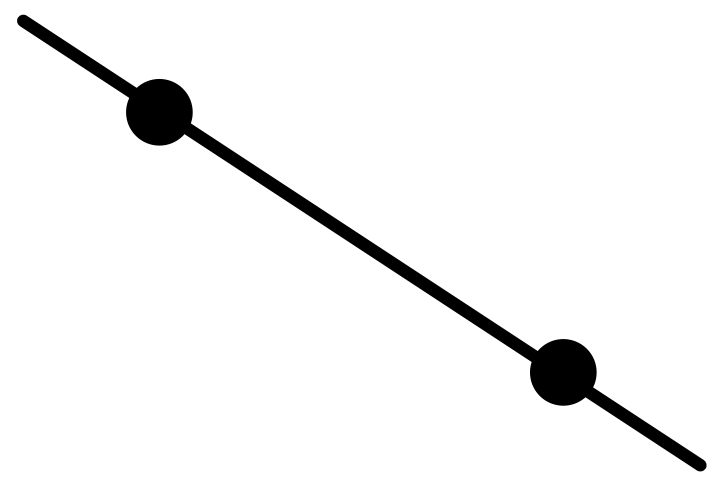
\includegraphics[width=.16\linewidth]{affine_combination.png}}\hfill
				\subfigure[Segment]{\label{fig:line-segment}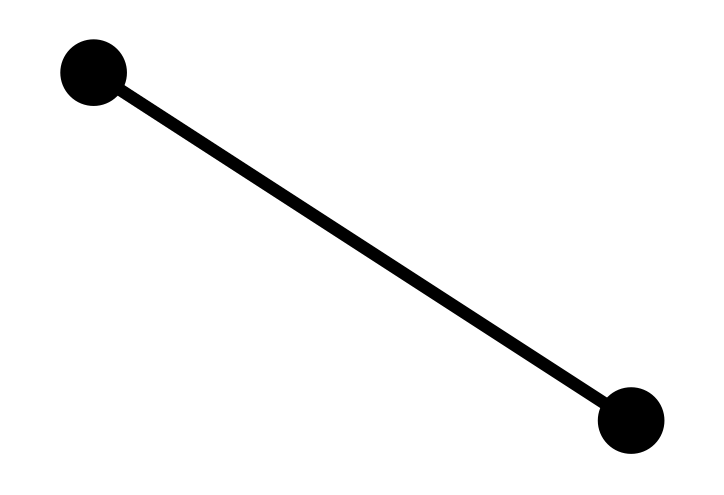
\includegraphics[width=.16\linewidth]{convex_combination.png}}\hfill
				\subfigure[Affine hull]{\label{fig:affine-hull}
\includegraphics[width=.16\linewidth]{affine_hull.png}}
	
				\subfigure[Convex hull]{\label{fig:convex-hull}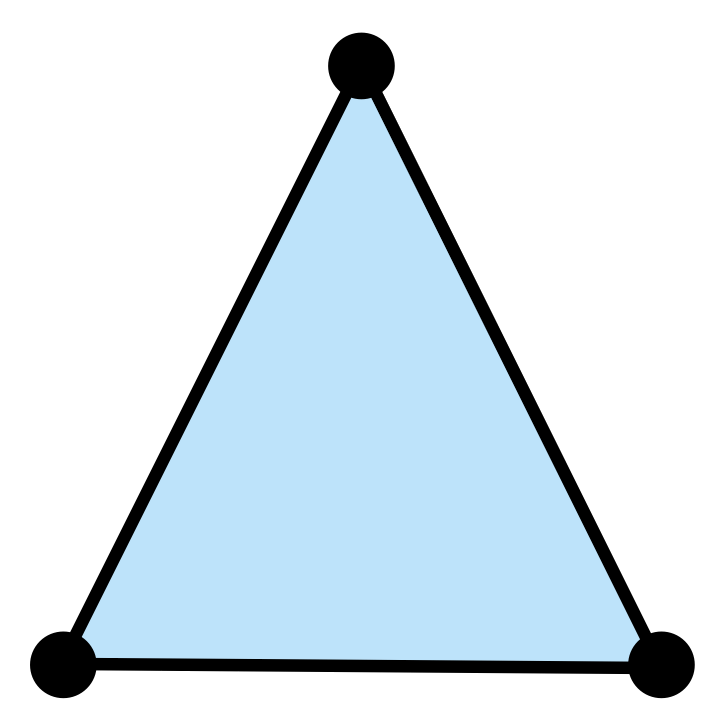
\includegraphics[width=.16\linewidth]{convex_hull.png}}\hfill
				\subfigure[Convex]{\label{fig:convex-not-polytope}
\includegraphics[width=.16\linewidth]{not_polytope.png}}\hfill
				\subfigure[Nonconvex]{\label{fig:nonconvex}
\includegraphics[width=.16\linewidth]{not_convex.png}}
			\end{minipage}
			%
			\caption{Pictorial representation of the definitions introduced in sec. \ref{sec:convexity}. Fig. \ref{fig:line} shows a line, which is an affine combination of two points. In \ref{fig:line-segment}, a line segment between (or a convex combination of) two points is shown. The affine hull of three noncollinear points is the plane (\ref{fig:affine-hull}), while the convex hull of a finite number of points defines a polytope (\ref{fig:convex-hull}). Any polytope is a polyhedron, but the converse is not true. Fig. \ref{fig:convex-not-polytope} shows a convex set with an infinite number of extremal points, therefore not a polytope. Nonconvex sets do not contain every line segment between its elements (\ref{fig:nonconvex}).}
		\end{figure*}


		% \begin{figure}[t!]
		% 	\centering
		% 	\begin{subfigure}{0.3\textwidth}
		% 		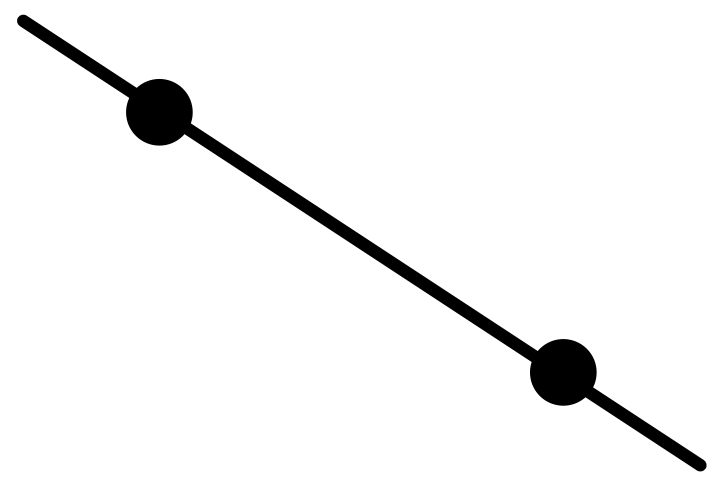
\includegraphics[width=.5\textwidth]{affine_combination.png}}
		% 	\end{subfigure}
		% 	\begin{subfigure}{0.3\textwidth}
		% 		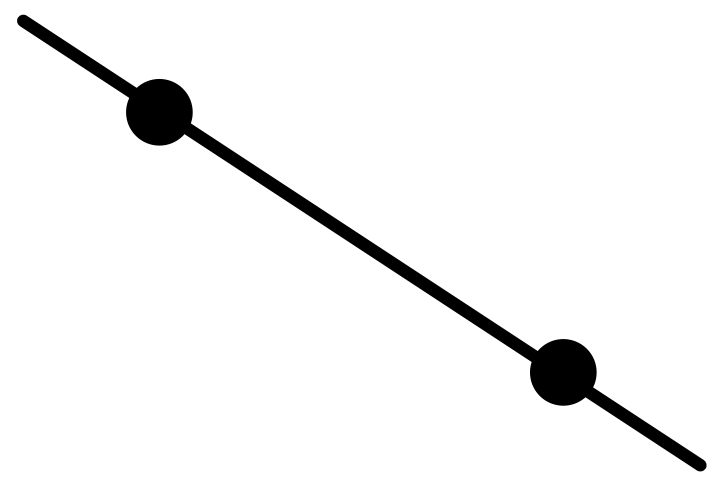
\includegraphics[height=.13\linewidth]{affine_combination.png}}
		% 	\end{subfigure}
		% 	\begin{subfigure}{0.3\textwidth}
		% 		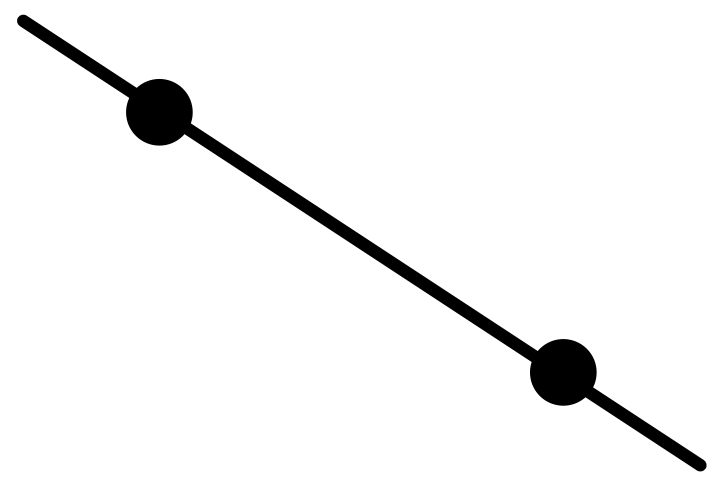
\includegraphics[height=.13\linewidth]{affine_combination.png}}
		% 	\end{subfigure}

		% 	\begin{subfigure}{0.3\textwidth}
		% 		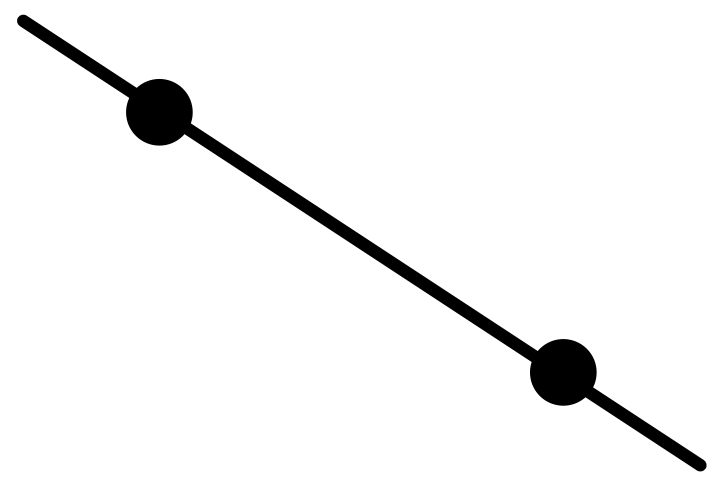
\includegraphics[height=.13\linewidth]{affine_combination.png}}
		% 	\end{subfigure}
		% 	\begin{subfigure}{0.3\textwidth}
		% 		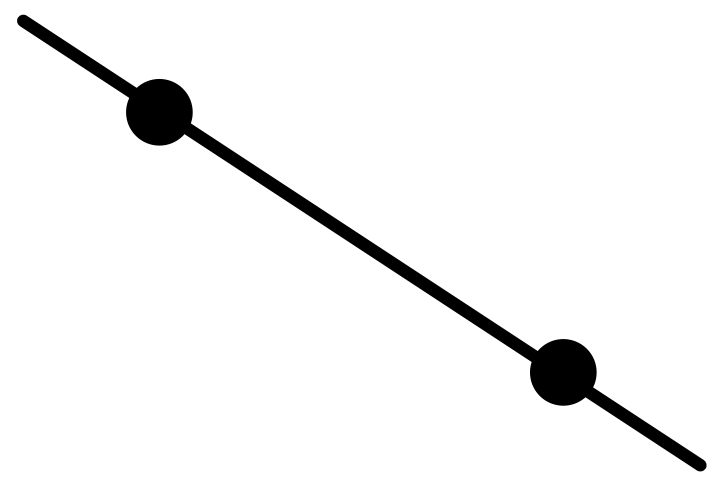
\includegraphics[height=.13\linewidth]{affine_combination.png}}
		% 	\end{subfigure}
		% 	\begin{subfigure}{0.3\textwidth}
		% 		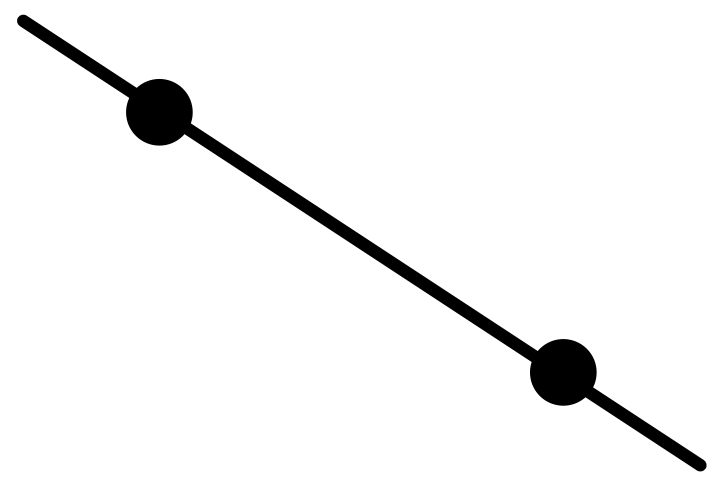
\includegraphics[height=.13\linewidth]{affine_combination.png}}
		% 	\end{subfigure}
		% 	%
		% 	\caption{Pictorial representation of the definitions introduced in sec. \ref{sec:convexity}. Fig. \ref{fig:line} shows a line, which is an affine combination of two points. In \ref{fig:line-segment}, a line segment (or a convex hull of two points) is shown. Two affine hull of three noncollinear points is the plane (\ref{fig:affine-hull}), while the convex hull of a finite number of points defines a polytope (\ref{fig:convex-hull}). Any polytope is a polyhedron, but the converse is not true. Fig. \ref{fig:convex-not-polytope} shows a convex set which is not a polytope. Is has an infinite number of extremal points. Nonconvex sets do not contain every line segment between its elements (\ref{nonconvex}).}
		% \end{figure}


		As much as cubes have vertices, edges and faces, polytopes have $k$-faces. Any \emph{face} $F$ of a polytope $P$ is a set
		$$
			F = P \,\cap\, \{ x \in \mathbb{R}^d \mid c^\intercal x = b \} ,
		$$
		where $c \in \mathbb{R}^d$ is a column-vector, $b \in \mathbb{R}$, and any $x \in P$ is such that $c^\intercal x \leq b$. Visually, a face is any intersection of $P$ with a closed halfspace that touches $P$ but is not inside of it. The dimension $k$ of the affine hull of $F$ goes into the name $k$-face. Faces of dimension $0$ and $1$ are vertices and edges, while faces of dimension $\text{dim} (P) - 1$ are especially named \emph{facets}. For a cube ($\mathbb{R}^3$), the facets would match the commonly called faces.

		Our previous definitions of polyhedra and polytopes are sometimes termed $\mathcal{H}$-polyhedra and $\mathcal{H}$-polytopes. An alternative that will later become important is that of $\mathcal{V}$-polytopes, which are defined as the the convex hull of a \emph{finite} set of points. After the convex hull is performed, they become the extremal points of the convex set. The $\mathcal{V}$-description of a unit square is $\mathcal{V} = \{ (0, 0), (1, 0), (0, 1), (1, 1) \}$, and after taking $\conv{\mathcal{V}}$ we get all points that, in the $\mathcal{H}$-description satisfy the linear system $Ax \leq b$ defined by 
		%
		$$
			A =
			\begin{pmatrix}
				-1 & 0 \\
				1 & 0 \\
				0 & -1 \\
				0 & 1
			\end{pmatrix},
			\quad\text{ and }\quad
			b =
			\begin{pmatrix}
				0 \\
				1 \\
				0 \\
				1
			\end{pmatrix} .
		$$
		%

		$\mathcal{H}$ and $\mathcal{V}$ representations can be proven mathematically equivalent (theorem 1.1 in \cite{ziegler_lecturespolytopes_1995}) but, computationally, the choice of description may significantly matter. As will be made explicit in chaps. \ref{chap:pam} and \ref{chap:pam-classical}, classicality in prepare and measure scenarios can be interpreted as the belonging of a behavior in a polytope. Conversely, nonclassicality may be witnessed through the violation of some inequality defining its facets. The $\mathcal{H}$-description of these polytopes is thence preferable for being more ergonomic. Finding these descriptions is important not only for prepare and measure scenarios, but are rather important in several other correlation scenarios. In Bell nonlocality scenarios, for instance, they are the celebrated Bell inequalities. Despite theoretical and practical importance, no general methods to directly build $\mathcal{H}$-descriptions of these polytopes are known. On the other hand, it is conceptually easy to enumerate all extremal points of classicality polytopes (the $\mathcal{V}$-description). Casting one to the other (i.e., performing the vertex or facet enumeration) can be done through specialized, user-friendly softwares such as \texttt{PANDA}, \texttt{lrs} and \texttt{cdd} \cite{PANDA,lrs,cdd} but, unfortunately, this is a computationally expensive problem that can only be done for the very simplest cases of interest. The conceptual significance of $\mathcal{H}$-descriptions will be further explored in chap. \ref{chap:pam}, and an example of description conversion will be discussed in chap. \ref{chap:pam-classical}. Results therein were obtained with \texttt{PANDA}, and descriptions of the algorithms and user guides can be found in the aforementioned references.

		A second important fact involving polyhedra and polytopes is that linear functions can be efficiently optimized inside them through so-called linear programming. In the remainder of this chapter, we go back to the problem posed in the introduction, and briefly discuss two efficiently computable instances of optimization problems, both of which are widely used in quantum information.


	%%%%%%%%%%%%%%%%%%%%%%%%%%%%%%%%%%%%%%%%%%%%
	\section{Optimization}

		Solving an arbitrary instance of eq.~\eqref{eq:optimization-program} is a hard problem, and general methods only exist for special instances of optimization programs. Convex optimization (\texttt{CONV}) --- which happens when all the $f_i$ are convex functions --- is one of the largest classes of programs that can be efficiently solved to global optimality. Even though $\texttt{LIN} \subset \texttt{SDP} \subset \texttt{CONE} \subset \texttt{CONV}$, specialized algorithms for subsets of convex optimization, such as conic (\texttt{CONE}), semidefinite (\texttt{SDP}) and linear (\texttt{LIN}) programming, renders even larger instances of those practical. Whilst we will not discuss them, the main reference for convex programming is the textbook \cite{boyd_convexoptimization_2004}, and a good reference for cone programming, tuned to quantum information, is \cite{uola_conic_2019}.

		Because of their use in the industry, ready-to-use solvers for optimization problems are broadly accessible. I will mention them in due time, but algorithms will not be introduced in depth. For thorough discussions, see, e.g., \cite{papadimitriou1998combinatorial,matousek2007understanding} for linear programming, \cite{vandenberghe_sdp_1996,gartner2012approximation} for SDPs and \cite{boyd_convexoptimization_2004} for convex optimization.


		%%%%%%%%%%%%%%%%%%%%%%%%%%%%%%%%%%%%%%%%%%%%
		\subsection{Linear programming}
		\label{sec:linear-programming}

			Linear programming happens when all the $f_i$ are linear functions. Recalling eq.~\eqref{eq:optimization-program}, you will see that the feasible region $\mathcal{F}$ is thence an intersection of halfspaces --- a polyhedron. Apart from being widely used in the industry to optimize supply chains, workforce allocation and delivery routes, it is also useful to search for probability distributions satisfying a set of constraints. The significance of this problem will become clearer in chap. \ref{chap:pam-classical}.

			Being linear, the objective function $f_0 : \mathbb{R}^n \mapsto \mathbb{R}$ can conveniently be written as $c^\intercal x$, where $c = (c_1, \ldots, c_n)$ is a constant vector in $\mathbb{R}^n$ defining the quantity to be maximized. Minimizing $c^\intercal x$ is the same as maximizing $-c^\intercal x$, so the discussion holds both ways. For an \emph{unconstrained} problem, there is not much more to say: just follow along the direction of the gradient. In this case, though, unless $f_0$ is constant, the program would end up being \emph{unbounded}. Things get more interesting when $x$ is constrained to be in a subset $\mathcal{F} \subset \mathbb{R}^n$. We can do that by saying $0 \leq x_i \leq 1, \,\forall i$, for instance, and then we would be optimizing $c^\intercal x$ over some hypercube. More generally, in linear programming we allow the constraints to be of the form $a_i^\intercal x \leq b_i$, where $a_i \in \mathbb{R}^n$ and $b_i \in \mathbb{R}$. There is no need to consider equality conditions separately, as we can just use two inequalities with inverted directions. So we do not have to write all constraints separately, a shorthand notation is to build an $m \times n$ matrix $A = [a_1 \; \ldots \; a_m]^\intercal$ and a vector $b = [b_1 \; \ldots \; b_m]^\intercal$ of bounds so that
			%
			\begin{subequations}
				\begin{alignat}{2}
					&\text{given}    &\quad & c, A, b \\
					&\underset{x}{\text{max.}}   &	  & c^\intercal x \\
					&\text{s.t.}    &      & Ax \leq b 
				\end{alignat}
				\label{eq:lp}
			\end{subequations}
			%
			is a general form of a linear program (LP). When $\mathcal{F} = \emptyset$, the program is \emph{unfeasible}, meaning there is no vector $x$ that satisfies the constraints. Requiring that $x_i \geq 1$ and $x_i \leq -1$ would certainly put you in that situation. If $\mathcal{F}$ is not empty, then the program may either have a solution or be unbounded. To understand why the latter may be the case, notice that $\mathcal{F}$ is a polyhedron. As such, it may itself be unbounded. Consider, for instance, $x \in \mathbb{R}^2$ with $\mathcal{F} = \{ 0 \leq x_1 \leq 1, x_2 \geq 0 \}$. If $c = [c_1 \; c_2]$, with $c_2 > 0$, the optimal value $p^*$ would go to infinity. On the other hand, $c_2 \leq 0$ would be alright even though $\mathcal{F}$ is unbounded. When $\mathcal{F}$ is a (nonempty) polytope, there is always some solution $p^*$ to the program. A solution is either unique (only a single $x^*$ leads to $p^*$), or there are infinitely many solutions yielding the same $p^*$. To understand why this is so, consider the \emph{fundamental theorem of linear programming}, which states that every feasible, bounded linear program has an optimal solution on a vertex of $\mathcal{F}$. If optimal solutions happen at two different vertices, then any $x$ in the line segment between them results in $p^*$. Otherwise, there would either be a larger feasible value in the segment, or the feasible region would not be convex. 

			Linear programs are efficiently solvable in practice. The simplex method, proposed by George Dantzig in 1947, builds upon the fact that optimal solutions occur in vertices. Starting from any basic feasible solution (a corner of $\mathcal{F}$), it smartly hops to neighboring vertices along edges that increase $f_0$. If you end up at a basic feasible solution connected to no edges that increase the objective value, or if you visit an unbounded edge, you are done. A rigorous presentation and complexity analysis of it can be found in \cite{papadimitriou1998combinatorial}, chap. 2. Interestingly, the simplex method is \emph{not} of polynomial time complexity (i.e., it is not efficient \emph{in theory}). Rather, there are families of linear programs for which it performs poorly. Nevertheless, it is a reliable and efficient method in practice, and is widely used (in several variations) up to this day. There are provably polynomial time algorithms in theory, of which the ellipsoid method --- invented in 1970 for nonlinear programming, then adapted and proved polynomial for linear programming in 1979 ---, was the first. Even so, it is not efficient in practice. The more recent interior-point methods are provably polynomial in theory, and fast in practice. Pedagogical discussions of these methods, together with historical remarks, are nicely presented in chap. 7 of \cite{matousek2007understanding}.

			Due to its wide applicability in the industry, there are many open source and proprietary linear programming solvers available, such as GLPK, Gurobi, and Mosek \cite{glpk,gurobi,mosek}. Most provide user-friendly interfaces to widely used programming languages, such as C, C++, Python and MATLAB. To further aid in using them, there are also modeling languages that can be used to specify programs in a high-level format, and that internally converts and dispatches the problem to specific solvers. YALMIP \cite{yalmip} and CVX \cite{cvx} are widely used inside MATLAB, while PICOS \cite{picos} and CVXPY \cite{cvxpy} are common choices when working in Python.	


		%%%%%%%%%%%%%%%%%%%%%%%%%%%%%%%%%%%%%%%%%%%%
		\subsection{Semidefinite programming}
		\label{sec:sdp}

			Semidefinite programming largely generalizes linear programming, and has found numerous applications in statistics, economics, control theory, pattern recognition and machine learning, to mention a few (see sec. 2 of \cite{vandenberghe_sdp_1996} and chap. 1 of \cite{boyd_convexoptimization_2004} for a survey). It is also widely used as a tool in approximation algorithms to graph theoretical problems \cite{gartner2012approximation}, and polynomial and non-commutative polynomial optimization \cite{npa_prl_2007,npa_njp_2008}; the latter being widely used in quantum information.

			While linear programming is the optimization of a linear function over a polyhedron, semidefinite programming is the optimization of a linear function over a spectrahedron. Before we further explain it, recall that
			$$
				S^m = \{ X \in \mathbb{R}^{m \times m} \mid X = X^\intercal \}
			$$
			is the set of $m \times m$ symmetric matrices, and
			$$
				S_+^m = \{ X \in S^m \mid X \succeq 0 \}
			$$
			the one of positive $m \times m$ semidefinite matrices. All eigenvalues of a symmetric ($X = X^\intercal$) matrix are real, and the positive semidefiniteness condition ($X \succeq 0$) further requires they must be nonnegative.

			Building upon the general linear program~\eqref{eq:lp}, we write a semidefinite program (SDP) as
			%
			\begin{subequations}
				\begin{alignat}{2}
					&\text{given}    &\quad & c, F_0, \ldots, F_n \\
					&\underset{x}{\text{max.}}   &	  & c^\intercal x \\
					&\text{s.t.}    &      & F_0 + \sum_{i=1}^n x_i F_i \succeq 0 .
				\end{alignat}
				\label{eq:sdp}
			\end{subequations}
			%
			Here, $F(x) \equiv F_0 + \sum_{i=1}^n x_i F_i \succeq 0$ is what we call a \emph{linear matrix inequality} (LMI), and it enforces the r.h.s. to be in $S_+^m$. The $n + 1$ matrices $F_0, \ldots, F_n$ are in $S^m$, and we maintain $x \in \mathbb{R}^n$. A semidefinite program is thus the optimization of a linear function $c^\intercal x$ under the constraint that $F(x)$ is positive semidefinite.

			This may seem like a rather arbitrary definition. To debunk this impression, first notice that if $F(x) \succeq 0$ and $F(y) \succeq 0$, then
			$$
				F[ \alpha x + (1 - \alpha) y ] = \alpha F(x) + (1- \alpha) F(y) \succeq 0
			$$
			for all $0 \leq \alpha \leq 1$. Thus, both the objective function and the constraint are convex, and semidefinite programming is a special case of convex optimization. More than that, $S_+^n$ is a convex cone (i.e., it is closed under conic combinations), meaning it is also a special case of conic optimization. Now it does not look that much arbitrary, but rather it seems too specialized. But it is not, for if we let $F_0 = \text{diag}(b)$ and $F_i = \text{diag}(a_i)$, we recover the form of a linear program just like eq.~\eqref{eq:lp}. Putting it all together, $\texttt{LIN} \subset \texttt{SDP} \subset \texttt{CONE} \subset \texttt{CONV}$, as stated in the beginning of this section.

			A general $F(x)$ may have a block-diagonal section of the form $\text{diag}(Ax + b)$, and a more general structure elsewhere. Thus, a linear matrix inequality represents an affine section of $S_+^n$, also called an \emph{spectrahedron}. Unlike polyhedra, they may have curved boundaries. A cylinder, for instance, can be parameterized as an $F(x)$ with $4 \times 4$ matrices \cite{vinzant_spectrahedron_2014}. A last interesting link to linear programming is that $F(x) \succeq 0$ if and only if $z^\intercal F(x) z \geq 0$ for all $z \in \mathbb{R}^m$. An SDP is thus a linear program with infinitely many linear constraints on $x$.

			The usefulness of semidefinite programming in quantum information is hinted by the fact that quantum states and measurement effects are positive semidefinite matrices. As long as the objective function is linear, we can optimize over them, and they have proven to be useful in quantum state discrimination \cite{bae_discrimination_2015}, quantum steering \cite{cavalcanti_2016_steering} and hierarchies for nonlocal correlations \cite{npa_prl_2007,npa_njp_2008}, among other applications. One of them will be shown in chap. \ref{chap:pam-quantum}. A drawback in dealing with density operators or measurement effects is that, while semidefinite programming is, as in here, usually discussed over the real field, quantum objects make use of complex numbers. One can nevertheless embed them in real variables. This can be a cumbersome task to do manually but, luckily, the modeling interfaces mentioned in the last section can do this under the hood before calling the solver.

			Semidefinite programming can also be efficiently solved both in theory and in practice. Interior-point methods are usually robust and efficient, and are implemented in some user-friendly solvers such as SDPA \cite{sdpa} and Mosek \cite{mosek}. Performance comparisons between these and several other SDP solver are available at \cite{performance_sdp_solvers}.


			%%%%%%%%%%%%%%%%%%%%%%%%%%%%%%%%%%%%%
			\subsubsection{Joint measurability robustness}
			\label{sec:incompatibility-robustness}

				The concept of joint measurability was introduced in sec. \ref{sec:measurements}. Following along the same notation, $\mathcal{M} = \{E_b^y \}_{b, y}$ is a set of $Y$ quantum measurements, indexed by $y$, each having $\mathcal{O}(y)$ outcomes. A parent measurement is called $J_\ell$, and only exists if $\sum_\ell J_\ell \delta_{b, \ell_y} = E_b^y$, where $\ell = \ell_1\ell_2\ldots\ell_Y$, and each $\ell_i \in \{ 1, \ldots, \mathcal{O}(i) \}$. From this requirement, it follows that $J_\ell$ can extract all information needed to reproduce $\mathcal{M}$. Whenever such a $J_\ell$ does not exist, $\mathcal{M}$ is incompatible, or not jointly measurable.

				More than determining whether an $\mathcal{M}$ is joint measurable, it is also interesting to ask to what extent a measurement is incompatible. Such \emph{incompatibility robustness} must be defined relative to \emph{something}. This something is what we call a noise model. Formally, a \emph{noise model} $\mathbf{N} : \mathcal{P}(d, \mathbf{n}) \mapsto \mathbb{S}(\mathcal{P}(d, \mathbf{n}))$ maps from the set of $Y = \abs{\mathbf{n}}$ $d$-dimensional POVMs, each with $\mathbf{n} = (n_1, \ldots, n_Y)$ outcomes, to the set $\mathbb{S}(\mathcal{P}(d, \mathbf{n}))$ of subsets of $\mathcal{P}(d, \mathbf{n})$. The simplest possible choice for $\mathbf{N}$ is the white noise model
				%
				$$
					\mathbf{N} = \Bigg\{ \Big\{ \frac{\id}{n_1} \Big\}_{i=1}^{n_1}, \ldots, \Big\{ \frac{\id}{n_Y} \Big\}_{i=1}^{n_Y} \Bigg\} ,
				$$
				%
				but several other common choices, such as depolarization maps or probabilistic noise also fit the definition. In general, it may also depend on $\mathcal{M}$, but we require that it contains at least one set of jointly measurable measurements. Adequateness is a matter of application, and different choices may lead to different results.

				Having the noise model fixed, we define the incompatibility robustness of $\mathcal{M}$, with respect to $\mathbf{N}$, as
				%
				\begin{equation}
				    \chi^*_\mathcal{M} = \sup_{\substack{\chi \,\in\, [0, 1]\\ \{ N_{b \mid y}\} \,\in\, \textbf{N}( \mathcal{M} )}} \Big\{ \chi \mid \chi \{ E_{b \mid y} \} + (1 - \chi) \{ N_{b \mid y} \} \in \textbf{JM} \Big\} .
				    \label{eq:incompatibility-robustness}
				\end{equation}
				%
				$\textbf{JM}$ denotes the set of all jointly measurable measurements, and $\chi^*_\mathcal{M} = 1$ readily implies $\mathcal{M}$ is jointly measurable. Any lower value means it is not, for to become it must be mixed with noise. More than that, if $\chi^*_\mathcal{M} < \chi^*_{\mathcal{M}^\prime}$ then $\mathcal{M}$ is \emph{more} incompatible than $\mathcal{M}^\prime$.

				Incompatibility robustness was investigated and applied in several works involving quantum measurements and more general quantum devices, such as \cite{heinosaari_noiserobustness_2015,designolle_robustness_2019,uola_onetoonesteering_2015}. Our presentation follows the very thorough investigation in \cite{designolle_robustness_2019}, where analytical and numerical results for several noise models are presented, and further references can be found. The fact that eq.~\eqref{eq:incompatibility-robustness} can be solved through semidefinite programming is also known. To see why this is so, first notice that, if we take a closed noise set, the supremum in \eqref{eq:incompatibility-robustness} becomes a maximum. Furthermore, $f_0 = \chi$, so we are indeed optimizing a linear function. The measurement effects, $\{ E_{b \mid y} \}$ and noise effects $\{ N_{b \mid y} \}$ are given, and $J_\ell$, an optimization variable, is a collection of PSD operators (i.e., the parent measurement's effects). They must be constrained to sum to the identity, and the parent's marginals must recover $\mathcal{M}$. These are semidefinite constraints, as more clearly seen by writing the program
				%
				\begin{subequations}
					\begin{alignat}{2}
						&\text{given}    &\quad &\{ E_{b \mid y} \}, \{ N_{b \mid y} \} \\
						&\underset{\chi, J_\ell}{\text{max.}}   &	  & \chi \\
						&\text{s.t.}    &      &  \sum_\ell J_\ell \delta_{b, \ell_y} = \chi E_{b \mid y}  + (1 - \chi) N_{b \mid y}, \quad\forall b, y \\
						&				&		& J_\ell \succeq 0 \\
						&				&		& \chi \leq 1 .
					\end{alignat}
					\label{eq:incompatibility-robustness-sdp}
				\end{subequations}
				%
				Notice that the constraints $\eta \geq 0$ and $\sum_\ell J_\ell = \id$ are not missing, but rather are automatically enforced by the first constraint and the fact that the noise set must have at least one jointly measurable element, such that $0$ will always be a lower bound. We will come back to this program in sec. \ref{sec:incompatibility-vs-classicality}, where it will be crucial to our proof that measurement incompatibility is not sufficient for nonclassicality in prepare and measure scenarios. Before getting to that, we must first learn what prepare and measure scenarios actually are.
	\part{Prepare and measure}
	\label{part:pam}
		\chapter{The prepare-and-measure scenario}
\label{chap:pam}

    The prepare-and-measure (PM) scenario is one of the simplest and most fundamental examples of correlation scenarios. In it, a preparation apparatus produces and then sends a physical system, over a communication channel, to a measurement device which reads out information from the received state. Wherefore, it is an adequate setting in which to investigate two of the most fundamental building blocks of physical theories: states and measurements.

    Differently from the more widely studied Bell nonlocality and EPR steering scenarios, a quantum prepare-and-measure experiment may behave nonclassically even in the absence of entanglement. Quantum behaviors in PM scenarios must then rely on other strictly quantum features, such as measurement incompatibility \cite{carmeli_racsincompatibility_2020} and non-orthogonality of states \cite{brunner_dimension_2013}, but the exact relations are still unknown.

    Other than quantum communication, a second resource that also leads to drastically different behaviors is whether the preparation and measurement devices are independent or not. There are, in general, three possible cases; namely, full independence, shared randomness and entanglement assistance. Together with either classical or quantum communication, this will lead to six inequivalent prepare-and-measure configurations.

    Prepare-and-measure scenarios are also the simplest correlation scenarios that presume communication, and, as such, should become an indispensable ingredient in quantum networks \cite{bowles_pamnetworks_2015,poderini_pamcriteria_2020}. As with other correlation scenarios, quantum behaviors in the PM scenario can be exploited to build informational protocols that show advantage over their classical counterparts (sec. \ref{sec:communication-protocols}). On a more fundamental aspect, they are at the core of proposed informational principles to quantum theory \cite{pawlowski_infocausality_2009,pawlowski_infocausalityreview_2011}, and of quantum ontologies \cite{spekkens_2005_contextuality}.

    In chapters \ref{chap:pam-classical} and \ref{chap:pam-quantum}, novel results regarding some of these settings will be presented. To build towards that end, we now discuss these many different instances of preparation and measurement devices, and show how this scenario can be seen as a physical implementation of two paramountly important communication protocols.

    %%%%%%%%%%%%%%%%%%%%%%%%%%%%%%%%%%%%%%%%%%%%%%%%
    \section{Prepare-and-measure behaviors}

        The simplest prepare-and-measure setup consists of two black-boxes. One is the preparation device P, handled by Alice, and the other the measurement device M, handled by Bob. Nothing about the inner workings of these devices is assumed \emph{a priori} (see \ref{chap:introduction}), except that P prepares and communicates a physical system to M, which extracts information from the received preparation by measuring it.
    
        Alice is allowed to interact with her device through a classical input $x \in \mathcal{X} \equiv \natrange{X} \equiv [X]$. Her choice may weight on the probability $\condprob{m}{x}$ with which a state labeled by $m \in \mathcal{S}$ is prepared. Here, $\mathcal{S}$ represents the set of possible preparations. This choice can be more intuitively understood as the message Alice aims to encode in her preparation.
        
        Similarly, Bob can choose a configuration $y \in \mathcal{Y} \equiv [Y]$ for the measurement device, which will thence output $b \in \mathcal{B} \equiv [B]$ with probability $\condprob{b}{m,y}$. This reflects the fact that the outcome of the experiment may be influenced by both the received message and Bob's choice of measurement (fig. \ref{fig:pam-scenario}). More intuitively, $Y$ limits how many choices of decoding procedures can be used by Bob to try and recover Alice's message $x$.

		\begin{figure}
			%
			\begin{minipage}[c]{0.41\textwidth}
				\centering
				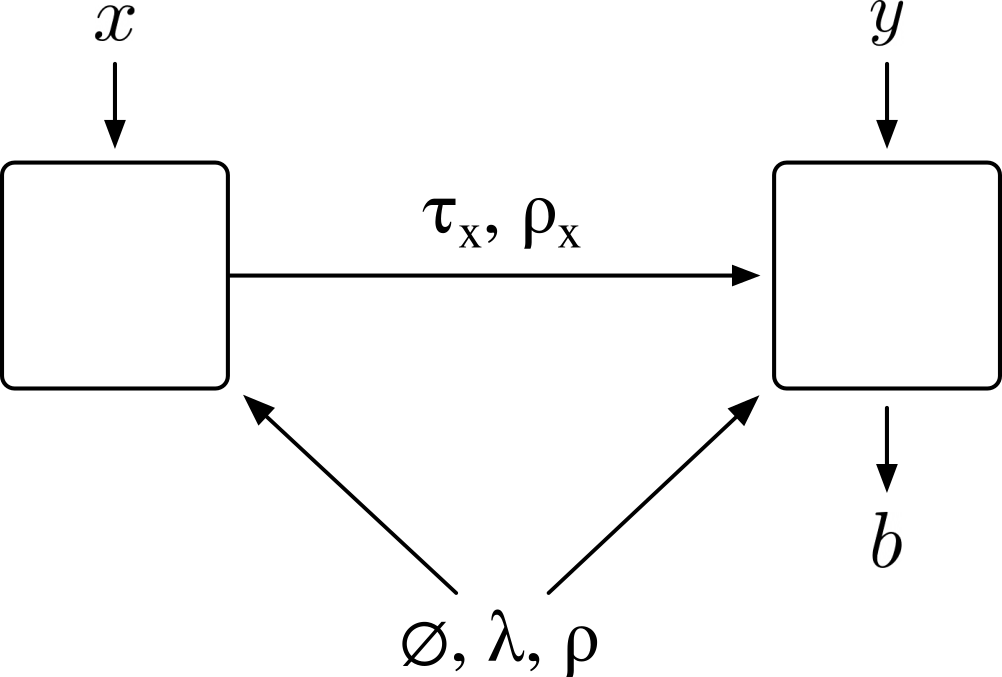
\includegraphics[width=.8\columnwidth]{pam_scenario.png}
			\end{minipage}
			%
			\begin{minipage}[c]{0.58\textwidth}
				\caption{Prepare-and-measure scenarios. The measurement box, upon receiving an input $x$, prepares either a classical, $\tau_x$, or quantum $\rho_x$, state to the measurement device. In turn, given a choice $y$ of measurement, an output $b$ is observed. From their causal past, the devices may be independent ($\emptyset$), share classical randomness ($\lambda$), or even quantum correlations ($\rho$).}	
				\label{fig:pam-scenario}
			\end{minipage}
			%
		\end{figure}

        A last, indispensable condition is that neither Alice nor Bob know what happens in each other's labs. In other words, she must have no knowledge of $y$, as this is a choice made in her causal future, and he cannot know what was her choice $x$ of preparation, as this trivializes the scenario in a sense that will soon be made clearer. Taken together, these constraints amount to saying that all communication between them is mediated by the message $m$. Given that our intention is to study how this communication influence the observed statistics, this is clearly a natural assumption.
        
        An \emph{round} is a single run of the protocol described above. After many such rounds, Alice and Bob are allowed to share their knowledge with each other, and together they can build the \emph{behavior} $\mathbf{p} = \{ \condprob{b}{x,y} \}_{b,x,y}$ of their devices. This behavior characterizes the prepare-and-measure \emph{experiment}. Naturally, each $\condprob{b}{x,y} \geq 0$ and $\sum_b \condprob{b}{x,y} = 1, \,\forall x,y$ or, equivalently, $\mathbf{p}$ is a collection of conditional probability distributions, one for any fixed choice of a pair of settings $(x,y)$.
        
        We now arrive at the central question of (semi)device-independent quantum information: if all we have is the behavior $\mathbf{p}$, with no (or restricted) access to the actual workings of the devices, can we still certify some property about the states, measurements, or other quantities of interest? For instance, could we, by only observing $\mathbf{p}$, affirm that P prepares quantum --- as opposed to classical ---, states? Or that M applies nonprojective measurements? In many cases, the answer, surprisingly, is \emph{yes}.
    
        %%%%%%%%%%%%%%%%%%%%%%%%%%%%%%%%%%%%%%%%%%%%%
        \subsection{Classical preparations}
        \label{sec:classical-behaviors}

            Quantum preparations may behave quite distinctly from classical preparations, and knowing how to tell them apart is of the essence for developing quantum communication protocols. An important open question regards the properties that allow some sets of preparations and measurements to behave nonclassically. In chapter \ref{chap:pam-classical}, I will discuss the problem of classical simulatability of quantum behaviors in reasonable generality, and prove that measurement incompatibility is not a sufficient condition for nonclassicality in the PM scenario. To make that discussion precise, we must begin by defining what it is that we will call classically-simulatable behaviors or, for shortness, \emph{classical behaviors}.
        
            Starting from the paradigmatic prepare-and-measure scenario, let us further impose that $\mathcal{S}$, the set of possible preparations, contains only \emph{classical states} (dits). Naturally, as this is a communication scenario, the dimension $\abs{\mathcal{S}}$ of the classical system used for encoding the states must be bounded, otherwise communication becomes trivial (i.e., Alice can perfectly encode her message $x$ and Bob can perfectly recover it) and all behaviors are possible.
            
            Our first aim is to investigate the set of behaviors that can be achieved when communicating $d$-dimensional classical systems, or rather, when  $\mathcal{S} = \posrange{d}$. They will, in general, also depend on $X$ (the size of Alice's input alphabet) and $Y$ (the number of choices for Bob's measurement). Letting this set of behaviors be $\mathcal{C}_{d,X,Y}$, our previous discussion implies that
            %
            \begin{equation}
                \mathbf{p} \in \mathcal{C}_{d,X,Y} \quad\Longleftrightarrow \quad \condprob{b}{x,y} = \sum_{m \in \mathcal{S}} \condprob{m}{x} \condprob{b}{m,y} \quad\forall b,x,y .
                \label{eq:pam-classical-independent}
            \end{equation}
            %
            Essentially, then, $\mathcal{C}_{d,X,Y}$ contains all behaviors that may occur when (i) the devices are \emph{uncorrelated}, (ii) the preparations are classical and (iii) with dimension at most $d$, (iv) Alice has $X$ preparation choices, and (v) Bob picks one out of $Y$ measurement settings.
            
            To simplify the notation, whenever $X$ and $Y$ are arbitrary or clear by context, the subscripts will be omitted.
            
            Briefly detouring, it is interesting to notice that model~\eqref{eq:pam-classical-independent} is very much in the spirit of ontological models \cite{spekkens_2005_contextuality,harrigan_2008_ontological,galvao_2009_economical}. To see that, consider $\mathcal{S}$ as a finite, dimension-bounded ontic state space, and $x$ as the preparation procedure. Then, $\condprob{m}{x}$ models our epistemic state. Similarly, if we take $y$ as a choice of measurement procedure, we may interpret $\condprob{b}{m,y}$ as the indicator function. In this way, any theory that only produces behaviors $\mathbf{p} \in \mathcal{C}_{d,X,Y}$ admits a dimension-bounded ontological model.
            
            Conditions (iii)--(v) above are pretty much natural for any communication scenario, but the case is different for (i) and (ii). While in many situations, such as when we have some trust on our devices, (i) is justifiable, it is not always safe to assume that the devices are uncorrelated. The worst-case scenario for classical variables is when P and M can share an unbounded amount of pre-established classical correlations. Such correlations must reside in the causal past of the experiment (fig. \ref{fig:pam-dag}), but even so, they can be used to achieve better performance in several communication protocols implemented in the PM scenario \cite{de_vicente_bound_2019}, and lead to quite different geometrical structures \cite{de_vicente_shared_2017,dallarno_robustness_2012}. Without knowledge on what information they share, the best we can do is to call it $\lambda$ and say that $\pi$ is some probability distribution over this random variable. As both devices can fully access $\lambda \in \Lambda$,
            %
            \begin{equation}
                \mathbf{p} \in \mathcal{C}_{d,X,Y}^\lambda \quad\Longleftrightarrow \quad \condprob{b}{x,y} = \int_{\Lambda} \sum_{m \in \mathcal{S}} \pi(\lambda) \condprob{m}{x,\lambda} \condprob{b}{m,y,\lambda} d\lambda \quad\forall b,x,y .
                \label{eq:pam-classical-sr}
            \end{equation}
            %
            Here, $\mathcal{C}_{d,X,Y}^\lambda$ is the set of behaviors we get from $\mathcal{C}_{d,X,Y}$ by allowing for shared randomness. As $\pi(\lambda) \geq 0$ and $\sum_\lambda \pi(\lambda) = 1$, eq.~\eqref{eq:pam-classical-sr} is actually telling us that $\mathcal{C}_{d,X,Y}^\lambda = \conv{\mathcal{C}_{d,X,Y}}$. More than that, a slight variation on Fine's theorem \cite{fine_hidden_1982} (or sec. 2.3 of \cite{scarani_bell_2019} for a more pedagogical discussion) can show that the set $\mathcal{C}_{d,X,Y}$ has a finite amount of extremal points, called deterministic strategies \cite{gallego_pam_2010,de_vicente_bound_2019}. They are the points given by eq.~\eqref{eq:pam-classical-independent} when the response functions are deterministic, i.e., when $\condprob{m}{x} = \delta_{m,f(x)}$ and $ \condprob{b}{m,y} = \delta_{b,g(m,y)}$, for some functions $f : \mathcal{X} \rightarrow [d]$ and $g : [d] \times \mathcal{Y} \rightarrow \mathcal{B}$ that are made precise in the aforementioned references. As $\mathcal{C}_{d,X,Y}^\lambda$ can now be seen as a convex hull of finitely many points, this proves that $\mathcal{C}_{d,X,Y}^\lambda$ is a polytope. Recalling the discussion in sec. \ref{sec:convexity}, we emphasize that $\mathcal{C}_{d,X,Y}^\lambda$ can thus be described by an intersection of half-spaces, which are given by the linear inequalities defining its facets. This description will turn out to be especially useful during chap. \ref{chap:pam-classical}, in which we will get back to this topic and work out an example that should clarify this discussion.

			\begin{figure}
			%
				\begin{minipage}[c]{0.31\textwidth}
					\centering
					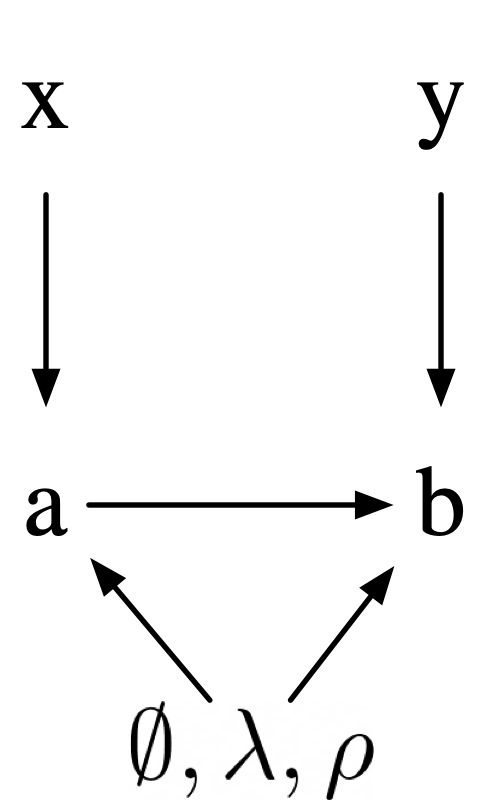
\includegraphics[width=.5\columnwidth]{pam-dag.png}
				\end{minipage}
				%
				\begin{minipage}[c]{0.68\textwidth}
					\caption{Causal structure of a prepare-and-measure experiment. Choice $x$ of preparation can only directly influence the message $m$, which can be encoded in a classical or quantum system. Communicating $m$ effectively screens-off the choice of $x$, unless the measurement device can perfectly recover it. Observable $b$ is influenced by the received message $m$ and the choice $y$ of measurement, which can be seen as a decoding function. Both $m$ and $b$ can be further classically or quantumly correlated by some variable in the causal past of the experiment.}	
					\label{fig:pam-dag}
				\end{minipage}
			\end{figure}
            
            For an example of the usefulness in understanding these sets, notice that for some fixed $X$ and $Y$, and some $d^\prime > d$, we have the proper inclusion $\mathcal{C}_{d} \subset \mathcal{C}_{d^\prime}$, which implies the same for the SR case. Ultimately, this means that larger dimensional communication can carry strictly more information. Now suppose that $W_d$ is a linear functional defining some facet of $\mathcal{C}_{d}^\lambda$ which is not a facet of $\mathcal{C}_{d^\prime}^\lambda$ (at least one such $W_d$ must exist, since $\mathcal{C}_{d}^\lambda \subset \mathcal{C}_{d^\prime}^\lambda$) and that, for any behavior $\mathbf{p} \in \mathcal{C}_d^\lambda$, we have a bound $W_d \cdot \mathbf{p} \leq C_d$. Because $W_d$ does not define a facet of $\mathcal{C}_{d^\prime}^\lambda$, there is some $\mathbf{p}^\prime \in \mathcal{C}_{d^\prime}^\lambda$ such that $W_d \cdot \mathbf{p}^\prime > C_d$. Hence, if we are given preparation and measurement boxes which are guaranteed to prepare only classical systems, and we observe some behavior that, like $\mathbf{p}^\prime$, violates the bound on $W_d$, we can certify that our uncharacterized devices is preparing states of dimension at least $d+1$.
            
            In disguise, I have exemplified what is called a (dimension) witness: any functional and bound that, (i) for some set of behaviors is never violated, but that (ii) can be violated by at least one behavior of some other set, is said to \emph{witness} some property. In our case, we are witnessing dimension in a semi device-independent fashion, as we have assumed the preparations are classical. Lastly, notice that the facets defining any $\mathcal{C}_d^\lambda$ polytope are, by definition, dimension witnesses. Furthermore, they are \emph{tight} witnesses, something which not all witnesses must be.
            
            For completeness, I note it is also possible to define a $\mathcal{C}_d^{\rho}$ set where the preparations remain classical, but the devices can be correlated through a shared quantum state $\rho$ \cite{tavakoli_eapam_2021,poderini_pamcriteria_2020}. When $\rho$ is an entangled state, it can lead to interesting behaviors associated with advantages in communication protocols \cite{pawlowski_earacs_2010}.
    
        %%%%%%%%%%%%%%%%%%%%%%%%%%%%%%%%%%%%%%%%%%%%%%
        \subsection{Quantum preparations}
        \label{sec:quantum-behaviors}

            To continue generalizing our discussion, let us also remove the assumption of classical preparations. 
            
            In that case, $\mathcal{S}$ will be a finite subset of $\mathcal{D}(\hilb)$, and $y$ a choice of quantum measurement. Employing Born's rule, we rewrite the behaviors as $\mathbf{p}_Q = \{ \tr{\rho_x E_{b \vert y}} \}_{b,x,y}$. Here, all $\rho_x \in \mathcal{S}$, and $\{ E_{b \mid y} \}_b$ is a POVM for each $y$. For the dimension bound, let $\text{dim}(\mathcal{S}) = \text{dim} \sum_{\rho_x \in \mathcal{S}}\text{supp}\left( \rho_x \right)$ be the smallest Hilbert space dimension needed to represent all density operators in $\mathcal{S}$. Then, in direct analogy to the classical behaviors sets, for any fixed $X$ and $Y$, we define $\mathcal{Q}_d$ as the set of behaviors for quantum communication with uncorrelated devices.
            
            Allowing for shared randomness introduces a slight change in the elements of the behaviors. Using the same notation as before, they turn into
            %
            $$
                \condprob{b}{x,y} =  \int_\Lambda \pi(\lambda) \tr{\rho_x^\lambda E_{b \vert y}^\lambda},
            $$
            %
            making it true that $\mathcal{Q}_d^\lambda = \conv{\mathcal{Q}_d}$ \review{Mas $\mathcal{Q}_d$ já é convexo, não? Então $\mathcal{Q}_d^\lambda = \mathcal{Q}_d$?}
            
            Lastly, and most importantly for chap. \ref{chap:pam-quantum}, Alice and Bob may share a quantum system $\rho \in \hilb_A \otimes \hilb_B$ and use it as a resource to improve their quantum communication. Most generally, Alice can use her share of $\rho$ as an aid in her encoding of $x$. The way to do it is by applying a local CPTP map $\Lambda_x$. As we must bound the communication to $d$-dimensional systems, $\Lambda_x : \mathcal{L}(\hilb_A) \rightarrow \mathcal{L}(\hilb_C)$, where $\hilb_C \simeq \mathbb{C}^d$. This system in $\hilb_C$ is then transmitted to Bob, who will afterwards hold $\rho_x = \left( \Lambda_x \otimes \id_B \right) \rho$. His measurements' effects act on $\hilb_C \otimes \hilb_B$. Behaviors compatible with experiments implementing this procedure are in the set $\mathcal{Q}^\rho_{d}$.
            
            Sometimes, it is a reasonable assumption to make $\hilb_A \simeq \hilb_C$ (see sec. \ref{sec:dense-coding} and chap. \ref{chap:pam-quantum}). Bear in mind, though, that it can lead to some loss of generality: recently, Tavakoli et al. \cite{tavakoli_eapam_2021} considered a qubit communication protocol where $4$-dimensional entanglement shows advantage over having only a $2$-dimensional entangled resource. To the best of my knoledge, those, together with Moreno et al.'s (\cite{moreno_pamdense_2021} and chap. \ref{chap:pam-quantum}), were the first results considering this most general quantum communication scenario.
            
            As a side note, although I have presented entanglement-assisted quantum communication scenarios as the most general kind of PM scenario, there are still further possible generalizations if we allow Alice's and/or Bob's inputs $x$ and $y$ to also be quantum variables \cite{guerini_distributed_2019}. These are interesting and little explored scenarios, but dealing with them is out of our scope.
            
            Clearly, any of the sets $\mathcal{Q}$, $\mathcal{Q}^\lambda$ and $\mathcal{Q}^\rho$ is contained in their respective larger-dimensional counterparts. Thence, the same observations made before make it possible to also derive \emph{quantum} dimension witnesses \cite{gallego_pam_2010}. Whereas witnessing dimension for classical or quantum preparations is already of practical and fundamental interest, we ideally want to also distinguish between classical and strictly quantum behaviors. To that end, it is useful to recognize that a set of pair-wise commuting density operators can only generate classically reproducible statistics. More precisely, if $\mathcal{S}_C$ is a set of $d$-dimensional density operators such that $\left[ \rho_i, \rho_j \right] = 0, \,\forall \rho_i, \rho_j \in \mathcal{S}_C$, then they can be simultaneously diagonalized w.r.t. some orthonormal basis $\{ \ket{ e_i } \}_{i=1}^d$. There can be at most $X=d$ $d$-dimensional preparations with this property. Letting $\rho_x = \sum_i c_{i,x} \ketbra{e_i}{e_i}$, we get that $\tr{ E_{b \mid y} \rho_x } = \sum_i c_{i,x} \braopket{e_i}{E_{b \mid y}}{e_i}$. Operationally, this means that communicating the label $x$ (a classical variable with dimension $X \leq d$) is enough to reproduce all possible behaviors: upon getting $x$ and Bob's choice $y$, the measurement device samples $\ket{e_i}$ with probability $c_{i,x}$, measures it considering $y$, and after collecting asymptotically many results the parties recover the correct $\condprob{b}{x,y}$.  
            
            As not all quantum states commute, it turns out that $\mathcal{C}_d \subset \mathcal{Q}_d$, and similarly for the sets allowing for shared randomness and entanglement assistance. Collecting the aforestated set relationships, we find that 
            %
            \begin{align}
                &\mathcal{C}_d \subset \mathcal{Q}_d \subset \mathcal{Q}_d^\lambda \subset \mathcal{Q}_d^\rho , \\
                &\mathcal{C}_d \subset \mathcal{C}_d^\lambda \subset \mathcal{Q}_d^\lambda \subset \mathcal{Q}_d^\rho, \\
                &\mathcal{C}_d \subset \mathcal{C}_d^\lambda \subset \mathcal{C}_d^\rho \subset \mathcal{Q}_d^\rho ,
            \end{align}
            %
            showing it is thus also possible to build nonclassicality witnesses for the prepare-and-measure scenario. Fig. \ref{fig:pam-behaviors} illustrates some of the set relationships discussed in this section.

			\begin{figure}
				%
				\begin{minipage}[c]{0.43\textwidth}
					\centering
	                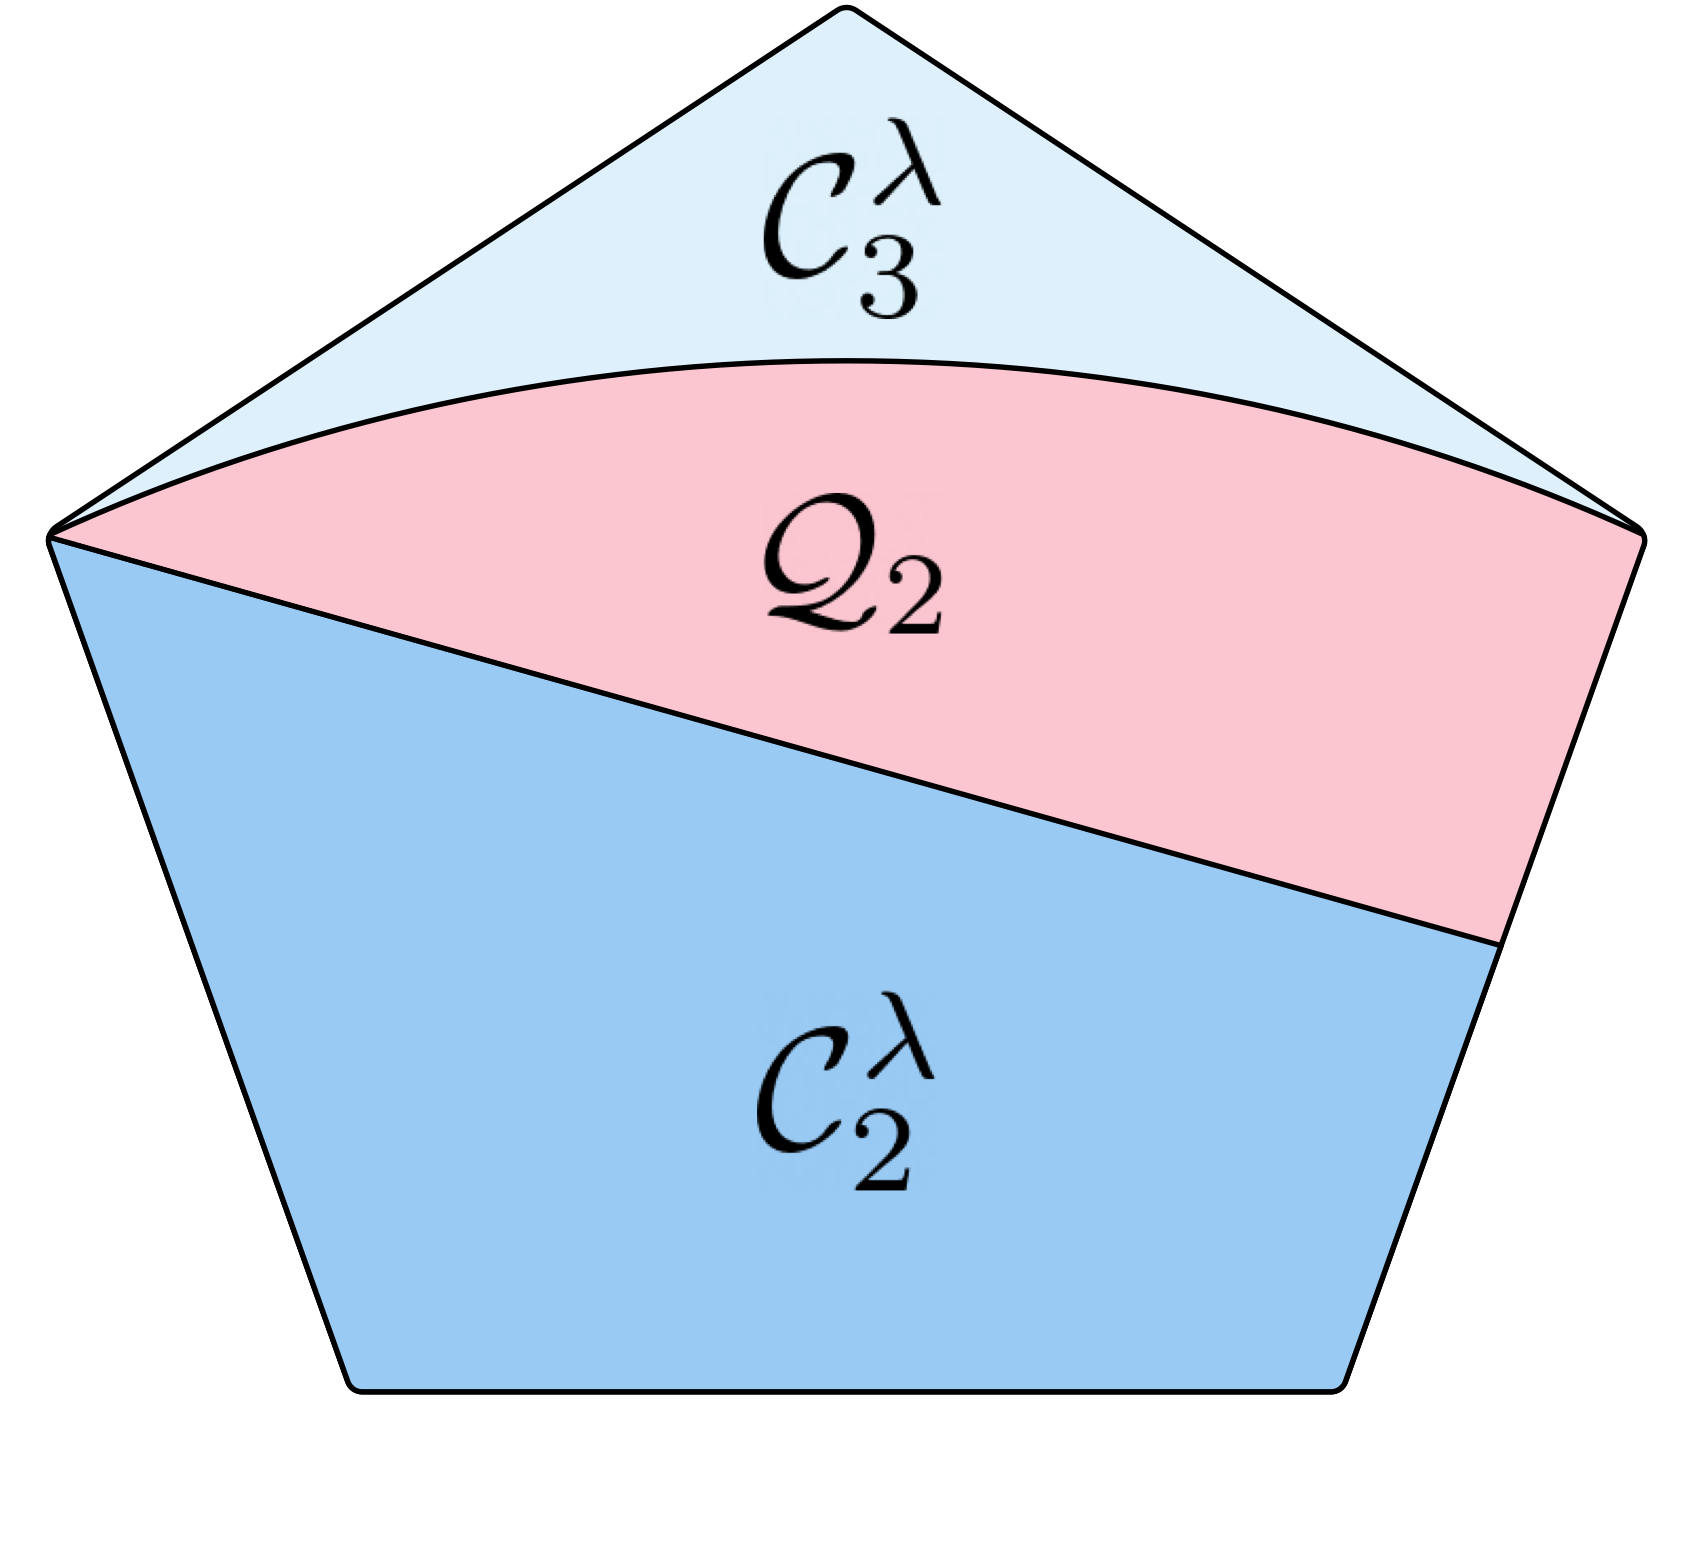
\includegraphics[width=.8\columnwidth]{behaviors.png}
			 	\end{minipage}
			 	%
				\begin{minipage}[c]{0.55\textwidth}
					\caption{Pictorial representation of prepare-and-measure behaviors. $\mathcal{C}_2^\lambda$, arising from $2$-dimensional classical communication with shared randomness, is a subset of any $\mathcal{C}_d^\lambda$ with $d > 2$ (eq.~\ref{eq:pam-classical-sr}). Qubit preparations, $\mathcal{Q}_2$, can behave in ways that violate the facets of $\mathcal{C}_2^\lambda$ \cite{gallego_pam_2010}.}	
            		\label{fig:pam-behaviors}
			    \end{minipage}
			    %
			\end{figure}
			            
            \ornamentbreak
            
            In recent years, a multitude of dimension and nonclassicality witnesses for prepare-and-measure scenarios have been proposed \cite{gallego_pam_2010,brunner_dimension_2013,sikora_dimension_2016,dallarno_robustness_2012,de_vicente_bound_2019,bowles_certifying_2014,wehner_lower_2008} and some of them experimentally tested \cite{hendrych_experimental_2012,ahrens_experimental_2012,dambrosio_highdimensional_2014}. More stringent conditions can also be used to perform self-testing of states and measurements, which can be used to certify the use of mutually unbiased bases, nonprojective measurements, or targeted sets of states \cite{tavakoli_selftesting_2018,farkas_selftesting_2019,wei_selftesting_2019,mironowicz_fouroutcome_2019,tavakoli_selftesting_2020,miklin_universal_2021,moreno_pamdense_2021}. All the while, known computational methods can aid in bounding the set of finite dimensional quantum correlations in prepare-and-measure scenarios \cite{navascues_bounding_2015,navascues_characterizing_2015}. The prepare-and-measure scenario and its sequential, or prepare-transform-and-measure variations \cite{mohan_sequential_2019,miklin_sequentialunsharp_2020} are also expected to serve as building blocks for quantum networks \cite{bowles_pamnetworks_2015,wang_pamnetworks_2019}. Complementing their versatility, they can also be seen as a physical implementation of many paradigmatic communication protocols such as random access coding and dense coding, which I now briefly introduce.


    %%%%%%%%%%%%%%%%%%%%%%%%%%%%%%%%%%%%%%%%%%%%%%
    \section{Prepare-and-measure communication protocols}
    \label{sec:communication-protocols}

        The preeminent practical interest in prepare-and-measure scenarios is due to the fact that quantum communication can beat classical protocols in many tasks that can me modeled as preparing and measuring states. These include cryptographic key distribution \cite{pawlowski_pamqkd_2011}, secret sharing \cite{schmid_secret_2005} and communication complexity scenarios \cite{buhrman_communicationreview_2010}. Simplifiedly, the latter deals with the question of how much is the least amount of communication needed to compute or approximate some function $f(x,y)$ where the inputs $x$ and $y$ are distributed. Prepare-and-measure scenarios clearly resemble this structure. All we have to do is to stipulate a figure of merit that, generally depending on $f$, measures how well some protocol performs. If we additionally manage to show some separation between the best performance achievable, for instance, in $\mathcal{C}_d^\lambda$ against $\mathcal{Q}_d^\lambda$, we can prove quantum advantage in the task. A special and widely studied choice of $f(x,y) = x_y$ leads us to the so-called \emph{random access coding} (RAC) protocol.

        \subsection{Random access coding}
        \label{sec:racs}

            An $\rac{n}{d}{m}$ random access code (RAC) is a communication task in which a party --- commonly Alice, --- is given a $n$-length $d$itstring $\mathbf{x} = x_1 x_2 \ldots x_n$, with each $x_i \in \{0, \ldots, d - 1 \}$, and required to encode it in another ditstring $\mathbf{a}$ of length $m$, where $m < n$.

            The $m$ dits representing $\mathbf{a} = \mathcal{E}(\mathbf{x})$, where $\mathcal{E} : \{0, \ldots, d - 1\}^n \mapsto \{0, \ldots, d - 1\}^m$ is an encoder function, are then sent to a second party, whom we'll call Bob. Bob is queried with an $y \in \{1, \ldots, n\}$ and must correspondingly guess what was the value of $x_y$. His guess may be modeled through $n$ decoding functions $\mathcal{D}_y : \{0, \ldots, d - 1\}^m \mapsto \{0, \ldots, d - 1\}$ that are chosen depending on the query $y$. We name \textit{encoding-decoding strategy} the ordered set $(\mathcal{E}, \mathcal{D}_{1},\ldots,\mathcal{D}_{n})$.

            When Alice and Bob use the same strategy in all rounds of the protocol, the observed statistics are always deterministic, i.e, the probability of Bob answering $b$ is given by $\condprob{b}{\mathbf{x}, y} = \delta\left[b, (\mathcal{D}_{y} \circ \mathcal{E})(\mathbf{x})\right]$, and in each round of a RAC, Bob's probability of guessing the right value is given by $p(b = x_y \mid \mathbf{x}, y)$.

            She and he must cooperate to guess as best as they can. Their performance is typically measured through the \emph{worst-case success probability} $p_{\text{worst}}$, defined as the minimum guess probability $p(b = x_y \mid \mathbf{x}, y)$ occurring for their particular encoding-decoding strategy. When the best possible strategy for an $\rac{n}{d}{m}$ scenario is such that $p_{\text{worst}} \leq 0.5$, the RAC is said to not exist, as in that case a better or equivalent performance could be achieved through independently guessing.

            Shared randomness is known to improve performance in this task. This is done by allowing the encoding and decoding functions to be correlated by some pre-established random variable $\lambda$. For a concrete example, consider the simplest $\rac{2}{2}{1}$ scenario. When no SR is allowed, $p_{\text{worst}} \leq 0.5$ \cite{ambainis_qracsoriginal_1999}. With SR, however, Alice and Bob can cooperate in the following way. Before each round, a random variable $\lambda \in \{0, 1\}$ instructs Alice to send $\mathbf{a} = x_\lambda$. Bob knows $\lambda$, so if he's queried with $y = \lambda$, he can answer correctly with certainty; otherwise he can just flip a coin. Of course, we still have $p_{\text{worst}} \leq 0.5$ in this situation. However, it is known from \cite{ambainis_srqracs_2009} that when SR is allowed, the best possible strategy is such that \review{Confirmar se é isso mesmo}
            %
            \begin{equation}
                p_{\text{worst}} = p_{\text{avg}} \equiv \frac{1}{nd^n} \sum_{\mathbf{x},y} \condprob{b=x_y}{\mathbf{x},y}
                \label{eq:rac-p-avg}
            \end{equation}
            %
            for an uniform distribution on $y$, proving that a $\rac{2}{2}{1}$ SR-RAC with $p_{\text{worst}} = 0.75$ exists.

            Something else that can further improve performance is allowing quantum communication. In this case, we interpret the encoders $\mathcal{E}(\mathbf{x}) = \rho_x \in \mathcal{D}(d)$ as preparation procedures and the decoders $\mathcal{D}_y = \{ E_{b \mid y} \}_b$ as quantum measurements.

            Quantum random access codes (QRACs) first appeared in \cite{wiesner1983conjugate} and were later rediscovered and linked to quantum automata in \cite{ambainis_qracsoriginal_1999}. With this popularization, multiple new results and experimental demonstrations regarding the existence and advantage of QRACs over their classical counterparts rapidly ensued \cite{nayak1999optimal,ambainis2002dense,hayashi_41qracs_2006,ambainis_srqracs_2009,spekkens2009preparation,pawlowski_pamqkd_2011}.

            Mapping QRACs to prepare-and-measure scenarios with quantum communication amounts to choosing $\abs{\mathcal{X}} = d^n$ preparations $\rho_{x} \in \mathcal{D}(d)$, and $\abs{\mathcal{Y}} = n$  choices of POVMs with $\abs{\mathcal{B}} = d$ outcomes each \cite{de_vicente_bound_2019}. The set of behaviors is then $\mathcal{Q}_{d,d^n,n}$, and optimizing the protocol means looking for a $\mathbf{p} \in \mathcal{Q}_{d,d^n,n}$ that maximizes either $p_{\text{worst}}$ or $p_{\text{avg}}$, depending on which is the chosen figure of merit. In the next chapter we will make use of this mapping to demonstrate an interesting quantum advantage activation phenomenon in QRACs.

            Additionally to RACs, SR-RACs and QRACs, one could also investigate SR-QRACs \cite{ambainis_srqracs_2009}, EA-RACs \cite{pawlowski_earacs_2010} and EA-QRACs, where ``EA'' stands for ``entanglement-assisted''. Each of these cases (which I'll herein collectively refer to as simply ``RACs'') could analogously be mapped to a PM scenario, and the optimal solutions would be searched for inside the PM behavior sets $\mathcal{C}$, $\mathcal{C}^\lambda$, $\mathcal{Q}$, $\mathcal{Q}^\lambda$, $\mathcal{C}^\rho$ and $\mathcal{Q}^\rho$, respectively, all with subscript $d,d^n,n$.

            To end this section I note that while RACs can be cast as an instance of prepare-and-measure, the inverse is not true. Investigating what different kinds of \emph{information retrieval tasks} \cite{emeriau_torpedo_2020} arise from such other instances could be an interesting research problem.

        %%%%%%%%%%%%%%%%%%%%%%%%%%%%%%%%%%%
        \subsection{Dense coding}
        \label{sec:dense-coding}

            Holevo's bound guarantees that $n$ qubits can perfectly encode no more than $n$ bits of information \cite{holevo-bound-1973}. Calling to mind that $n$ qubits require $2^n - 1$ complex coefficients to be fully described, this result comes to be tremendously surprising. Looking more closely, the setting where this conclusion arises from is a prepare-and-measure scenario with quantum communication but independent devices. Another seminal result proves that when the devices are not independent, but rather, share a maximally entangled state as a resource, it becomes possible to communicate two bits by sending a single qubit.

            Dense coding was first proposed by Bennett and Wiesner \cite{bennett_1992_superdense} similarly to the following argument. Let Alice and Bob share a two-qubit maximally entangled state $\ket{\Phi^+} = \frac{1}{\sqrt{2}} \sum_{i = 0}^{1} \ket{ii}$ (the same argument is valid for any unitary transformation of it). Her task is to communicate one out of four messages to Bob. We label those messages with choices from the ordered set $\mathcal{X} = (0, 1, 2, 3)$, which could be perfectly encoded with two bits. They previously agree on some special set of transformations, hereby $\Lambda = (\id,\sigma_x, \sigma_y, \sigma_z)$ --- where $\sigma_i$ are the Pauli matrices ---, to represent the respective encodings. Alice's encoding of $x$ is a simple matter of applying $\Lambda_x$ to her share of $\ket{\Phi^+}$. After receiving her qubit, Bob will have the state $\left( \Lambda_x \otimes \id \right) \ketbra{\Phi^+}{\Phi^+}$. The four possibilities are mutually orthogonal, thus can be perfectly distinguished by some suitable measurement (e.g., a standard Bell-basis measurement). He will hence be able to recover $x$ from a single communicated qubit.
            
            Purposefully, I have framed the protocol in the previously introduced notation for a prepare-and-measure scenario with quantum communication and entanglement assistance. My intention was to suggest that dense coding can be implemented as a special instance of prepare-and-measure scenarios, as it indeed can. More than that, several generalizations of this protocol are possible. The most straightforward ones are to allow for higher dimensional communication and entanglement \cite{bennett_1992_superdense} or mixed-state entanglement \cite{barenco_dense_1995}. More recently, discussions have been opened in regard to unbounded entanglement \cite{tavakoli_eapam_2021} or even dense coding protocols with errors \cite{nayak_rigidity_2020,moreno_pamdense_2021}. Chapter \ref{chap:pam-quantum} will detailedly discuss how we can use insights from prepare-and-measure scenarios to study the latter case. \comment{I plan to do the formal definition on chap. 5 because even if I did it here I'd probably have to repeat it there. That's why I didnt make it already but I can put it here as well if it's better...}
		\chapter{Classicality in the prepare-and-measure scenario}
\label{chap:pam-classical}

    A key objective in the study of quantum correlations is understanding what makes some behaviors be surely quantum, while others may be not. Progress on this issue improves our understanding of what is ``quantum'' in quantum theory, which in turn will lead to improved or even innovative technological applications.

    In this chapter, I introduce novel methods for deciding whether some set of quantum preparations or quantum measurements behaves classically. These will, in turn, provide new insights about a nonclassicality activation phenomenon and the relation between measurement incompatibility and quantum behaviors in prepare-and-measure scenarios.

    These results were published in \cite{degois_2021_general}, and computational details are provided in appendix \ref{ap:a}.

    \ornamentbreak

    To make the problem we want to solve precise, let us first recall that  the most general prepare-and-measure behaviors involving strictly classical variables are those in $\mathcal{C}^\lambda_{d,B,X,Y}$ (eq.~\eqref{eq:pam-classical-sr}).  Contrastingly, the $\mathcal{Q}_{d,B,X,Y}$ contain the \emph{least} general quantum behaviors, which are those needing only quantum preparations with independent devices (sec. \ref{sec:quantum-behaviors}). The relation $\mathcal{C}_{d,B,X,Y}^\lambda \subset \mathcal{Q}_{d,B,X,Y}$  reflects the fact that some behaviors arising from quantum preparations are nevertheless in $\mathcal{C}_{d,B,X,Y}^\lambda$, while others are definitely not. Those which are, can be simulated by classical preparations with shared randomness. Hereafter, we will call any behavior in the $\mathcal{C}^\lambda_{d,B,X,Y}$ \emph{classically reproducible/simulatable} --- or just \emph{classical}, for short.

    It is important to keep in mind that several distinct notions of classicality exist in the literature. As is the case of entanglement measures, some applications may call for a classicality model or another. Our choice of $\mathcal{C}_{d,B,X,Y}^\lambda$ for the classical behaviors set is general in the sense discussed in chap. \ref{chap:pam}. It is also in line with widely studied classicality models in different correlation scenarios, such as local hidden variables and local hidden states models \cite{brunner_2014_nonlocality,uola_2020_steering,cavalcanti_2016_steering}.

    Suppose a behavior $\mathbf{p}$ arose from a set $\mathcal{S}$ of quantum preparations under some collection of measurements, and furthermore that it is classically reproducible with \emph{d}its. This means that $\mathbf{p} \in \mathcal{C}_{d,B,X,Y}^\lambda$. But it does \emph{not} mean that $\mathcal{S}$ always behaves classically, for it may be the case that different measurements would reveal nonclassicalities in $\mathcal{S}$. Even if we certify $\mathcal{S}$ is classical for all possible sets of $Y$ measurements, it could happen that increasing the number of measurement choices leads to nonclassicality \cite{poderini_pamcriteria_2020}. To better understand what makes quantum preparations behave classically of not, we must then deal with any number of uncharacterized measurements. This is precisely the task we partially solve in sec. \ref{sec:preparation-classicality}. %Certifying that $\mathcal{S}$ is classical for unbounded $Y$ (i.e., irrespective of which and how many measurements Bob may employ) is precisely the task we aim to solve in sec. \ref{sec:preparation-classicality}.

    Before tackling that, it is both instructive and useful to further examine the $\mathbf{p} \in \mathcal{C}_{d,B,X,Y}^\lambda$ membership problem. As previously discussed, any $\mathcal{C}_{d,B,X,Y}^\lambda$ is a polytope, thus set membership can be certified through compliance with a finite set of linear inequalities representing its facets. If one is given the facets, this a computationally easy problem, but obtaining the facets is not. The whole complexity of the problem then lies in characterizing a the polytope for a given scenario. As first noticed in \cite{gallego_pam_2010}, this can be done by enumerating all of $\mathcal{C}_{d,B,X,Y}^\lambda$'s extremal points and finding their convex hull (see sec. \ref{sec:convexity}). The extremal points --- also called \emph{deterministic behaviors/strategies} ---, are found from eq.~\eqref{eq:pam-classical-independent} when the response functions are deterministic, and their enumeration can be cast as the following procedure.

    Let $\mathbf{p}_D = \left( p(b \mid x, y) \right)_{b, x, y}$ be an ordered list representing a deterministic behavior. To simplify the notation, let us consider $b \in \{ 0, 1\}$ (the generalization is straightforward) and write $\mathbf{p}_D = \left( \mathbf{v}_x \right)_{x=1}^X$, where $\mathbf{v}_x = \left( p(b = 0 \mid x, 1), \ldots, p(b = 0 \mid x, Y ) \right)$ will be called a \emph{substring}. Only the $b=0$ probabilities must be considered, as $p(1 \mid x, y) = 1 - p(0 \mid x, y)$. A deterministic behavior is valued as $1$ for one of the outcomes and, of course, $0$ for all others. Whenever $d = X$, there will be $2^{XY}$ distinct $\mathbf{p}_D$ vectors. In this $B=2$ case, those are exactly all possible $XY$-length $d$itstrings but, in the general case, there will be $B^{XY}$ vectors corresponding to only those $(B-1)XY$-length $d$itstrings with a single $1$ in each $B-1$-length consecutive substring. We can think of each of these vectors as a deterministic strategy where Alice's choice of $x$ is unambiguously encoded in a classical state $\tau_x$, from which Bob may then perfectly recover $x$ through classical post-processing. The nontrivial case happens when $d < X$, i.e., when there are only $d$ distinct classical preparations. As the preparation box has more buttons than distinct classical states, at least $\lceil X/d \rceil$ inputs will be mapped to the same message. Whenever $\tau_i = \tau_j$, obviously $\mathbf{v}_i = \mathbf{v}_j$, hence our vector $\mathbf{p}_D$ will have $d - X$ repeated substrings. With this in mind, enumerating all possible deterministic points amounts to generating every unique $dY$-length ditstrings, then repeating $d-X$ substrings $\mathbf{v}_x$ in all possible arrangements.

    The number of deterministic points scales exponentially as $N_\lambda \propto (B-1)^{dY}$, which makes the change to the hyperplane description intractable for all but the smallest parameters. One solvable case that will be used in sec. \ref{sec:nonclassicality-activation} is for $\mathcal{C}^\lambda_{2,2,4,2}$, where the polytope is defined by the two following classes of nontrivial inequalities \cite{poderini_pamcriteria_2020}
    %
    \begin{subequations}
        \begin{gather}
            S = E_{11} - E_{12} - E_{21} + E_{22} - E_{31} - E_{32} + E_{41} + E_{42} \leq 4 \label{eq:inequality-s}\\
            S^\prime = E_{11} + E_{12} + E_{21} - E_{22} - E_{41} \leq 3 
        \end{gather}
    \end{subequations}
    %
    where the $E_{xy}=\condprob{b=0}{x,y}-\condprob{b=1}{x,y}$ are the so-called \emph{correlators}.

    Framing it with quantum preparations, this scenario corresponds to a set $\mathcal{S}$ with $X=4$ possible $d=2$-dimensional quantum systems (qubits) that will be prepared by Alice's device then measured by Bob's. He will have $Y=2$ choices of POVMs, where each POVM is composed of $B=2$ effects. An interesting fact in this scenario (as well as many others) is that some quantum preparations and measurements, even with independent devices, can violate inequalities $S$ or $S^\prime$. When this happens, the behavior is not classically reproducible. In many cases, nonclassicalities provide quantum advantage in informational protocols (sec. \ref{sec:communication-protocols}). 

    %%%%%%%%%%%%%%%%%%%%%%%%%%%%%%%%
    \section{Classicality of preparations}
    \label{sec:preparation-classicality}

        But we are interested in a much more general question than that of certifying whether or not a \emph{behavior} is classically reproducible, namely, that of certifying if the set $\mathcal{S}$ of quantum preparations is itself classical. For that to be true, there must be no measurements that upon acting on $\mathcal{S}$ end up in a nonclassical behavior. Brute-forcing our way into the answer is off the table, for this would amount to testing the behaviors of $\mathcal{S}$ for \emph{all} (infinitely many) possible measurements.

        This is a similar problem to that of finding local hidden variable models for entangled states in Bell scenarios \cite{acin_2006_grothendieck,hirsch_2017_betterlocalhidden}, for which a general computational method guaranteeing a sufficient condition has recently been proposed \cite{cavalcanti_generalmethod_2016,hirsch_algorithmic_2016}. We now adapt it to the prepare-and-measure scenario.

        Suppose that, for the quantum states in $\mathcal{S}$ and a finite set $\mathcal{M} = \{ E_{b \mid y} \}_{b,y}$ of $Y$ measurements, the classical model~\eqref{eq:pam-classical-sr} exists, i.e., that
        %
        \begin{equation}
            \tr{\rho_x E_{b\mid y}} = \int_{\Lambda} \sum_{m = 1}^{d} \pi(\lambda) \condprob{m}{x,\lambda} \condprob{b}{m,y,\lambda} d\lambda \quad\forall b,x,y .
        \label{eq:quantum-classicality-model}
        \end{equation}
        %
        From trace's linearity, for any convex sum of effects,
        %
        \begin{equation*}
            \trb{\rho_x \left( w E_{b\mid y} + (1-w) E_{b^\prime \mid y^\prime} \right)} = w\tr{\rho_x E_{b\mid y}} + (1-w) \tr{\rho_x E_{b^\prime \mid y^\prime}} .
        \end{equation*}
        %
        Whence, $\mathcal{S}$'s behaviors are classical under all measurements in $\conv{\mathcal{M}}$, and in particular for all measurements whose effects are inside the largest ball we can inscribe in $\conv{\mathcal{M}}$ (fig. \ref{fig:measurements-hull}). For normalized Bloch vectors (c.f. eq.~\eqref{eq:normalized-bloch-vector-representation}), $0 \leq \eta \leq 1$ will be its radius. This ball is nothing but a depolarized Bloch ball $\eta \, \blochballd{d}$. This suggests that by probing the preparations with but a finite number of measurements and (possibly) finding a classical model, we can nevertheless certify classicality for the infinitely many measurements whose effects are in $\eta \, \blochballd{d}$. They can be written as
        %
        \begin{equation}
            \Phi_\eta(E_{b \mid y}) = \eta E_{b \mid y} + (1 - \eta) \frac{ \tr{E_{b \mid y}} }{d} \id \equiv E_{b \mid y}^\eta,
            \label{depolarized-measurements}
        \end{equation}
        %
        but they are still not all possible measurements. As an example, unless $\eta = 1$, many rank-1 projective measurements (those on the Bloch sphere) will be left out.

		\begin{figure}
		%
			\begin{minipage}[c]{0.42\textwidth}
				\centering
            	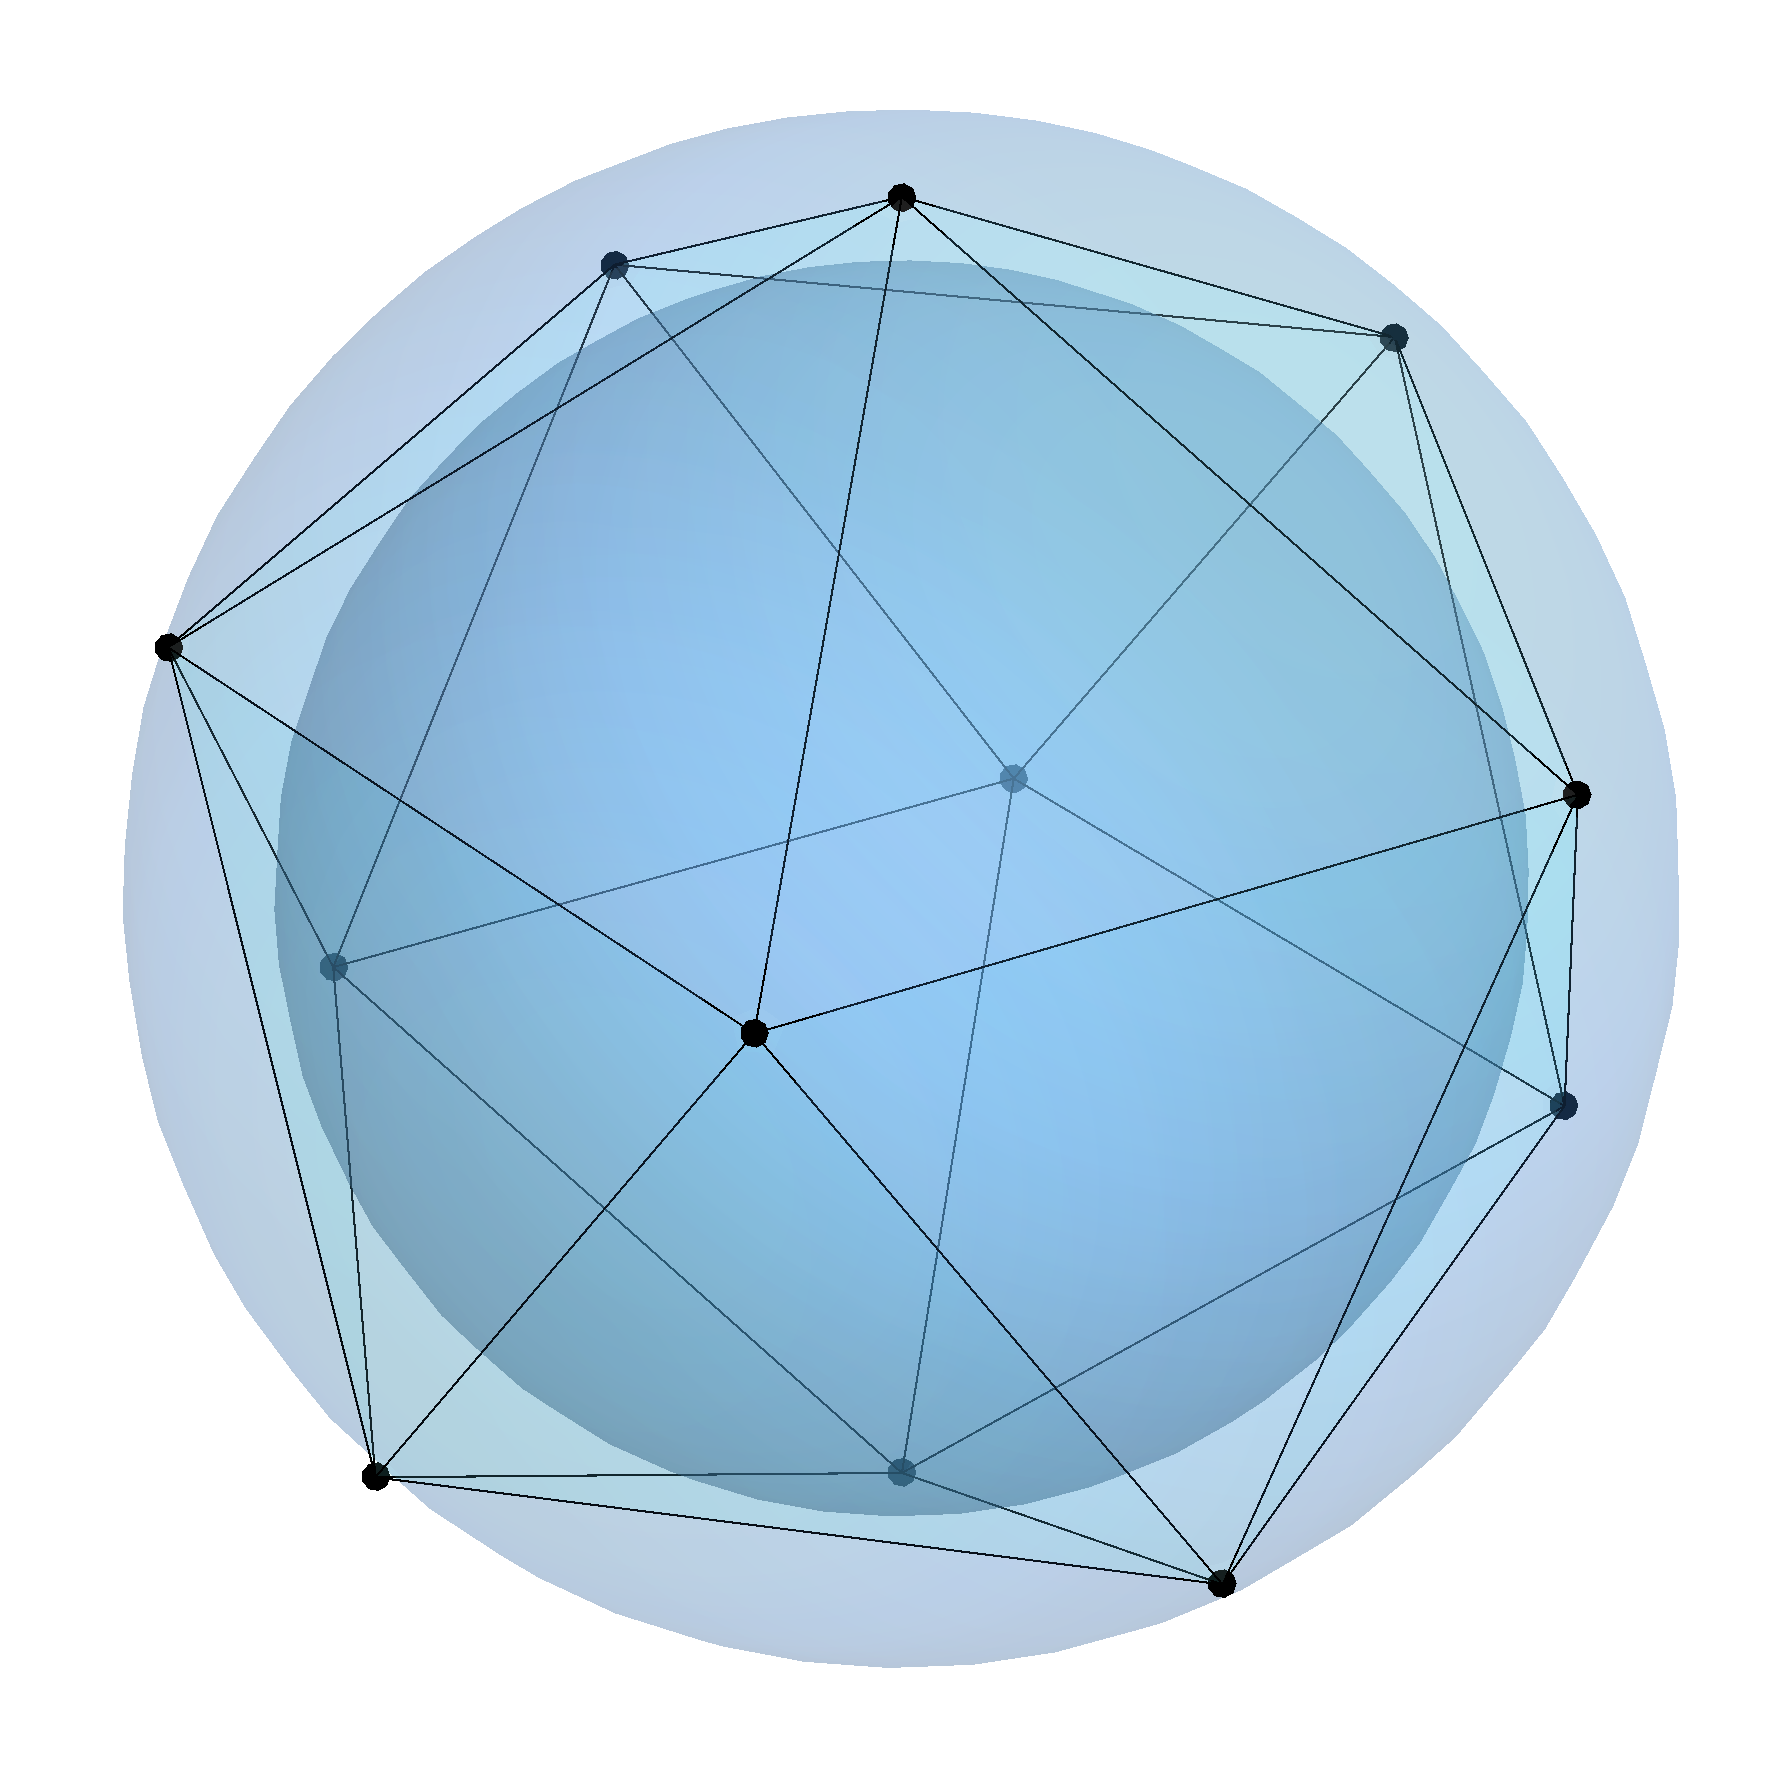
\includegraphics[width=.9\columnwidth]{measurements-hull.png}
			\end{minipage}
			%
			\begin{minipage}[c]{0.56\textwidth}
            	\caption{Representation of the method for $d = 2$. Each vertex on the Bloch sphere represents a measurement operator. To every $\Pi_{0 \vert y}$ we associate a corresponding antipodal $\Pi_{1 \vert y}$. Measurements inside the set enclosed by $\textbf{conv}(\mathcal{M})$ can be simulated by mixing these extremal ones. In particular, any measurement $\{ \Pi_{b \vert u}^\eta \}_b$ in a ball with radius $\eta$ inscribed in the polytope is simulable in such manner.}
   		    	\label{fig:measurements-hull}
			\end{minipage}
		\end{figure}

        The work-around is to consider the dual map $\Phi_\eta^\dagger$ applied to the preparations. This will result in each
        %
        \begin{equation}
            \rho_x \mapsto \Phi_\eta^\dagger(\rho_x) = \frac{1}{\eta} \left[ \rho_x - (1 - \eta) \frac{\id}{d} \right] \equiv O_x .
            \label{eq:polarized-preparations}
        \end{equation}
        %
        Analyzing the behavior of the $O_x$ under the $E_{b \mid y}^\eta$ tells us that
        %
        \begin{align*}
            \tr{O_x E_{b \mid y}^\eta} &= \text{tr}\left\{ \frac{1}{\eta} \left[ \rho_x - (1 - \eta) \frac{\mathbf{1}}{d} \right]  \left[ \eta E_{b \mid y} + (1 - \eta) \frac{ \tr{E_{b \mid y}} }{d} \id \right] \right\} \\
            &= \tr{\rho_x E_{b \mid y}} - \left[ \frac{1 - \eta}{d} - \frac{ 1 - \eta }{ d \eta }  + \frac{ (1 - \eta)^2 }{ d \eta } \right] \tr{E_{b \mid y}}.
        \end{align*}
        %
        If all effects $E_{b \mid y}$ are rank-1 projectors, then $\tr{E_{b \mid y}} = 1$ (sec. \ref{sec:gell-mann}), making it true that
        %
        \begin{equation}
            \tr{O_x E_{b \mid y}^\eta} = \tr{\rho_x E_{b \mid y}}.
            \label{eq:trace-equality-preparation-classicality}
        \end{equation}

        The procedure to test $\mathcal{S}$ for classicality follows from precisely this trace equality relation. We start out by defining an operator $O_x$ for each state $\rho_x \in \mathcal{S}$. Ensuingly, we probe the $\mathcal{O} = \{ O_x \}_x$ with some set $\mathcal{M} = \{ E_{b \mid y} \}_{b,y}$ of rank-1 projective measurements. If the model on the r.h.s. of eq.~\eqref{eq:quantum-classicality-model} exists for $\mathcal{O}$ and $\mathcal{M}$, the preceding discussion reveals it also exists for every measurement in $\conv{\mathcal{M}}$. It will then be true that $\mathbf{p} = \Big\{ \tr{O_x E_{b \mid y}^\eta} \Big\}_{b,x,y}$ is a classical behavior for \emph{all} measurements whose effects can be written as $E_{b \mid y}^\eta$. In turn, eq.~\eqref{eq:trace-equality-preparation-classicality} implies that the $\rho_x$ admit a classical model for all $E_{b \mid y}$, which are all rank-1 projections. Measurement results for projections of larger rank can be inferred from rank-1 projections through coarse graining (classical post-processing), hence the result is valid for all projective measurements.

        To cast this procedure as an optimization problem, recall that the deterministic strategies $\lambda$ can be enumerated as discussed in the previous section. Assuming that is done, the integral in~\eqref{eq:quantum-classicality-model} turns into a finite sum. Besides, the distance from the nearest hyperplane in the convex hull of $\mathcal{M}$ to the origin is $\eta$. Further observing that the maximally mixed state $\id/d$ is trivially classical, we write
        %
        \begin{subequations}
            \begin{alignat}{2}
                &\text{given}    &\quad & \mathcal{S},\, \mathcal{M},\, \eta, \{ \lambda \} \\
                &\underset{\pi(\lambda)}{\text{max.}}   &	  & \alpha \\
                &\text{s.t.}    &      & \alpha \rho_x + (1 - \alpha)\frac{\mathbf{1}}{d} = \eta O_x + \left( 1 - \eta \right) \frac{\mathbf{1}}{d}, \quad\forall x \label{eq:cond-1}\\
                &                  &      & \text{tr}(E_{b \vert y} O_x) = \sum_{m, \lambda} \pi(\lambda) p(m \vert x, \lambda) p(b \vert m, y, \lambda), \quad\forall b, x, y \label{eq:cond-2}\\
                &				   &	  & 0 \leq \alpha \leq 1 \\
                &				   &	  & \pi(\lambda) \geq 0 \\
                &				   &	  & \sum_\lambda \pi(\lambda) = 1 \label{eq:cond-5}.
            \end{alignat}
            \label{eq:preparation-classicality-projective}
        \end{subequations}
        %        
        Allowing the $\rho_x$ to be mixed with the identity in the l.h.s. of eq.~\eqref{eq:cond-1} guarantees the program will always have a feasible solution. Constraints \eqref{eq:cond-2}--\eqref{eq:cond-5} force the local model to exist, the mixtures to be valid density operators, and $\pi$ to be a probability distribution over the deterministic strategies, respectively. Any solution where $\alpha = 1$ certifies that preparations in $\mathcal{S}$ admit a classical model for all projective measurements. On the other hand, any $\alpha < 1$ certifies only that the preparations $\alpha \mathcal{S} = \{ \alpha \rho_x \}_x$ are classical. This criterion turns from sufficient to both necessary and sufficient only when $\eta \rightarrow 1$, a regime approachable by increasing the number $Y$ of probe measurements.

        Being a linear program (sec. \ref{sec:linear-programming}), eq.~\ref{eq:preparation-classicality-projective} can be efficiently solved up to numerical precision. Regardless of linear programming complexity, an instance of program~\eqref{eq:preparation-classicality-projective} has $N_\lambda$ variables. As already noted, $N_\lambda \propto (B-1)^{dY}$ thus the program size scales exponentially with the number of measurements. It will always be of interest to maximize $\eta$, and consequently, to maximize $Y$. With $X=4$ preparations, a common desktop computer can usually only handle less than $Y = 12$ projective qubit measurements. This limitation can be circumvented through the iterative optimization procedure described in sec. \ref{ap:a-computational}, which was applied in all upcoming results.

        It is also possible to extend our criterion to non-projective measurements. Dichotomic projective measurements are the extremal two-outcome POVMs. Consequently, out method actually guarantees classicality for all $B=2$-outcome measurements. For all other cases, we can extend it by simulatating POVMs with projective measurements (c.f. sec. \ref{sec:measurements}). To see how, recall that any set of generalized measurements $\mathcal{M} = \{ E_{b \mid y} \}_{b,y}$ becomes projective-simulatable after a certain amount $t$ of depolarization Observing that
        %
        \begin{equation}
            \trb{E_{b \mid y} \Phi_t(\rho_x)} = \trb{\Phi_t(E_{b \mid y}) \rho_x}
        \end{equation}
        %
        leads us to conclude that testing $\mathcal{S} = \{ \rho_x \}_x$ for classicality under all POVMs is the same as certifying that preparations
        %
        \begin{equation}
            \rho^\prime_x \equiv \Phi_t^\dagger \left( \rho_x \right) = \frac{1}{t} \left( \rho_x - \frac{1-t}{d} \id \right)
        \end{equation}
        %
        are classical for all projective measurements, where $t$ is some amount of depolarization such that $\Phi_t(\mathcal{M})$ are projective-simulatable.

        Program~\eqref{eq:preparation-classicality-projective} can be easily modified to this case by either adding an extra constraint or through explicit rewriting. For the former, it reads
        %
        \begin{subequations}
            \begin{alignat}{2}
                &\text{given}    &\quad & \mathcal{S},\, \mathcal{M},\, \eta, \{ \lambda \}, t \\
                &\underset{\pi(\lambda)}{\text{max.}}   &	  & \alpha \\
                &\text{s.t.}    &      & \rho_x^\prime = \frac{1}{t} \left( \rho_x - \frac{1-t}{d} \id \right), \quad\forall x \\
                &               &      & \alpha \rho_x^\prime + (1 - \alpha)\frac{\mathbf{1}}{d} = \eta O_x + \left( 1 - \eta \right) \frac{\mathbf{1}}{d}, \quad\forall x \\
                &                  &      & \text{tr}(E_{b \vert y} O_x) = \sum_{m, \lambda} \pi(\lambda) p(m \vert x, \lambda) p(b \vert m, y, \lambda), \quad\forall b, x, y \\
                &				   &	  & 0 \leq \alpha \leq 1 \\
                &				   &	  & \pi(\lambda) \geq 0 \\
                &				   &	  & \sum_\lambda \pi(\lambda) = 1 ,
            \end{alignat}
            \label{eq:preparation-classicality-povm}
        \end{subequations}
        % 
        which is also a linear program.


        %%%%%%%%%%%%%%%%%%%%%%%%%%%%%%%%%%%%%%%%%%%
        \subsection{Nonclassicality activation and quantum advantage in a RAC}
        \label{sec:nonclassicality-activation}

            Nonclassicality activation phenomena have been long-known in Bell scenarios, where an entangled state that only behaves locally may have its nonlocality activated, for instance, by local filtering, broadcasting, or by exploring multiple copies of the state \cite{popescu-filtering-1995, hirsch-hidden-2013,gallego2014nonlocality,navascues-activation-2011, palazuelos-superactivation-2012,cavalcanti2011quantum,bowles2020singlecopy}. Very recently, two interesting, similar phenomena were explored in PM scenarios \cite{poderini_pamcriteria_2020} --- one related to increasing the number of allowed measurements, and the other to the number of preparations. Our method can be applied to demonstrate a stronger form of the latter.

            Let us start by defining $\mathcal{S}(\alpha, \theta) = \{ \rho_{\mathbf{r_1}}, \rho_{\mathbf{r_2}}, \rho_{\mathbf{r_3}}, \rho_{\mathbf{r_4}} \}$ as the preparation set illustrated in fig. \ref{fig:preparation-set-activation}. They are parametrized by $\alpha$ --- a shrinking factor from the surface of the Bloch sphere ---, and the angle $\theta$. For the probe measurements, we will choose the ones parametrized by the Bloch vectors $\mathbf{q}_1 = (- \mathbf{x} + \mathbf{z}) / \sqrt{2}$ and  $\mathbf{q}_2 = (\mathbf{x} + \mathbf{z}) / \sqrt{2}$. Substituting back into inequality $S$ (eq.~\eqref{eq:inequality-s}), we get that $S(\alpha, \theta) = 4\sqrt{2} \alpha \sin \theta$. This curve is shown in fig. \ref{fig:nonclassicality-activation}, where any violation of $S \leq 4$ certifies nonclassicality.

            Our second step is to take every subset of $3$ preparations from $\mathcal{S}(\alpha, \theta)$ at some $\theta$. For each possibility, we run program~\eqref{eq:preparation-classicality-projective} and find the largest $\alpha^*$ such that \emph{any} collection of $3$ preparations is classical. Any $\alpha < \alpha^*$ has more of the identity state, thus preserves classicality. Sweeping $\theta$, we obtain the dotted curve shown in fig. \ref{fig:nonclassicality-activation}. The shaded region then corresponds to a situation where all triads of preparations are classical, but that taken together have their nonclassicality activated.

			\begin{figure*}[t!]
				\newdimen\subfigcapmargin  \subfigcapmargin  =  -3em
				\centering
				%
				\subfigure[Preparations]{\label{fig:preparation-set-activation}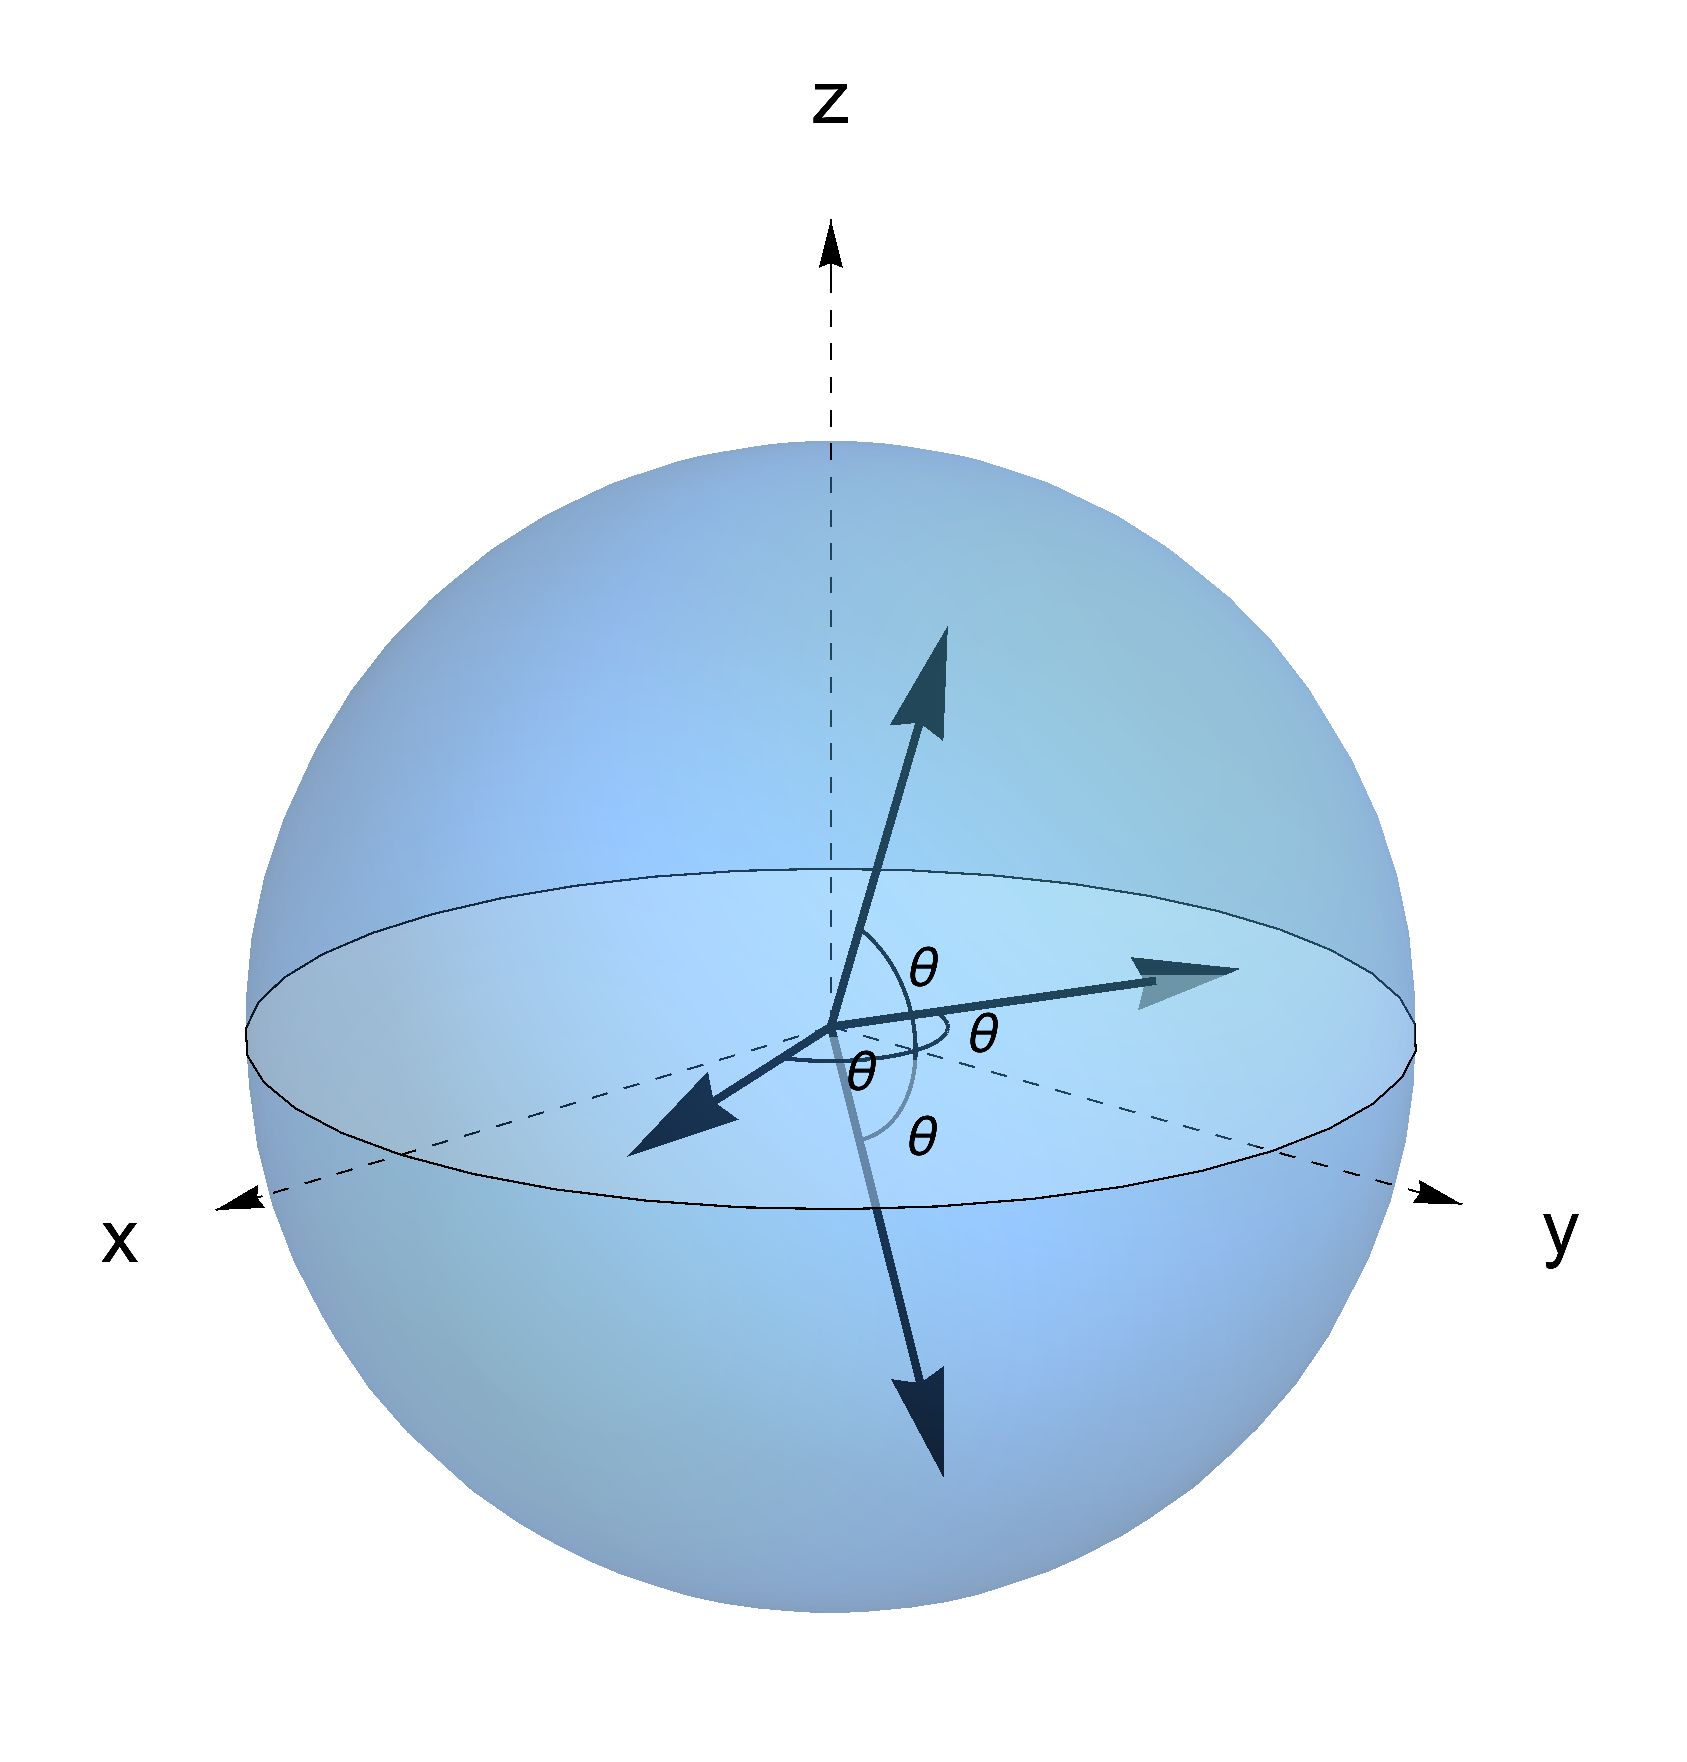
\includegraphics[width=.4\linewidth]{preparation-states.png}}\hfill
				\subfigure[Activation]{\label{fig:nonclassicality-activation}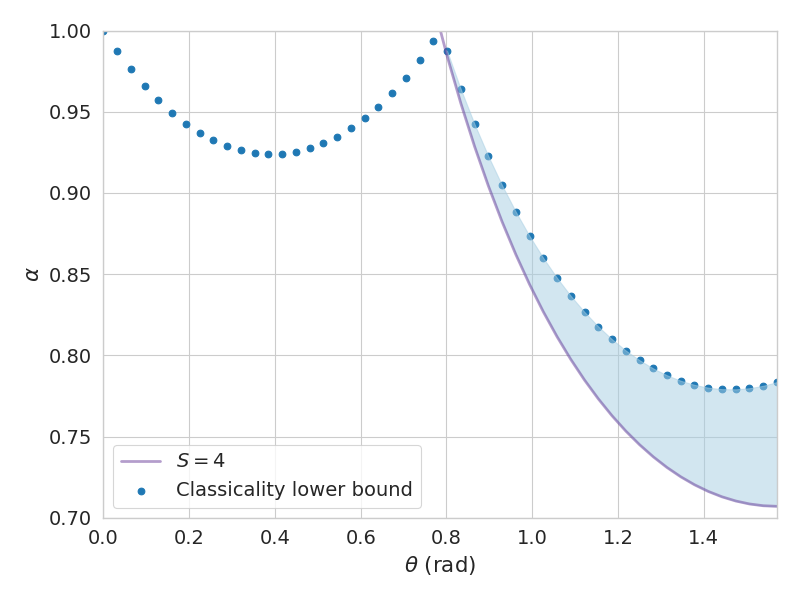
\includegraphics[width=.58\linewidth]{preparation-activation.png}}\hfill
				%
				\caption{Nonclassicality activation in the prepare-and-measure scenario. On the left, preparations $\mathcal{S}(\alpha, \theta) = \{ \rho_{\mathbf{r_1}}, \rho_{\mathbf{r_2}}, \rho_{\mathbf{r_3}}, \rho_{\mathbf{r_4}} \}$ are represented by their Bloch vectors, for $\alpha=0.8$. At $\theta=0$, all preparations are at $\alpha \mathbf{y}$. For $\theta = \pi/2$, $\mathcal{S} =  \{ -\alpha\mathbf{x}, \alpha\mathbf{x}, -\alpha\mathbf{z}, \alpha\mathbf{z} \}$, corresponding to the largest violation of inequality \eqref{eq:inequality-s}. On the right, result of applying program \ref{eq:preparation-classicality-projective} to $\mathcal{S}$. To run it, $12$ probe measurement effects arranged as the vertices of a rhombicuboctahedron ($\eta \approx 0.86$). As $S \propto \alpha$, every preparation set above the $S=4$ curve is non-classical. On the other hand, the classicality curve shows the maximum visibility such that any triad of states in the preparation set are classical. The shaded region thence represents sets of four preparations that are three-wise classical, but that that when taken together behave nonclassically. In this sense, nonclassicality is activated by measurement inclusion.}
			\end{figure*}
            
            The significance of this results can be illustrated when considering a $\rac{2}{2}{1}$ RAC. Section \ref{sec:racs}) tells us it can me mapped to a $(d,B,X,Y) = (2,2,4,2)$ prepare-and-measure instance, which is exactly the case for the class of inequalities represented by $S$. A \emph{class} is a collection of inequalities that are equivalent through symmetries. In correlation scenarios, these symmetries are called \emph{relabelings}. Because the labels attached to outcomes, preparations and measurements are arbitrary, inequalities obtained from another through relabeling $b$, $x$ and/or $y$ are equivalent. In particular, $s = E_{11} + E_{12} + E_{21} - E_{22} - E_{31} + E_{32} - E_{41} - E_{42} \leq 4$ is a relabeling of $S$. Borrowing from \cite{pawlowski_pamqkd_2011}, we note that, for the $\rac{2}{2}{1}$ RAC, the average probability of success \emph{is} the facet $s$. To see that, let's relabel preparations $\left( 1, 2, 3, 4 \right) \mapsto \left(00, 01, 10, 11\right)$ and open up
            %
            \begin{align*}
                        p_{\text{suc}}^{\text{avg}} &= \frac{1}{8} \sum_{\mathbf{x}, y} p(b = x_y \vert x_0 x_1, y) \\
                        \begin{split}
                            &= \frac{1}{8} \big[ p(0 \vert 00, 0) + p(0 \vert 00, 1) + p(0 \vert 01, 0) + p(1 \vert 01, 1) + \\
                            &\quad\qquad + p(1 \vert 10, 0) + p(0 \vert 10, 1) + p(1 \vert 11, 0) + p(1 \vert 11, 1) \big]
                        \end{split}
                        \\
                        \begin{split}
                            &= \frac{1}{8} \big[ p(0 \vert 00, 0) + p(0 \vert 00, 1) + p(0 \vert 01, 0) - p(0 \vert 01, 1) + \\
                            &\quad\qquad - p(0 \vert 10, 0) + p(0 \vert 10, 1) - p(0 \vert 11, 0) - p(0 \vert 11, 1) + 4 \big]
                        \end{split}
            \end{align*}
            %
            Switching $s$ to full-form and applying normalization, we get
            %
            \begin{align*}
            \begin{split}
                s &= 2 \big[ p(0 \vert 00, 0) + p(0 \vert 00, 1) + p(0 \vert 01, 0) - p(0 \vert 01, 1) + \\
                &\qquad\qquad - p(0 \vert 10, 0) + p(0 \vert 10, 1) - p(0 \vert 11, 0) - p(0 \vert 11, 1) \big] ,
            \end{split}
            \end{align*}
            %
            and together,
            %
            \begin{equation}
                p_{\text{avg}} = \frac{1}{8} \left( \frac{1}{2} s + 4 \right) = \frac{s + 8}{16} \leq \frac{3}{4} ,
                \label{eq:s-vs-pavg}
            \end{equation}
            %
            where the classical bound for $s$ was substituted in the last term. This relation means that any violation of $s$ in the $(2,2,4,2)$ PM scenario can be associated with a quantum advantage in the corresponding $\rac{2}{2}{1}$ QRAC. We have numerically found a lower bound for the maximum quantum violation of $s$ to be approximately $5.65685$. Substituting into eq.~\eqref{eq:s-vs-pavg}, $p_{\text{avg}} \approx 0.853553$, exactly matching the result found in sec. 3.3.1. of \cite{ambainis_srqracs_2009}. This also suggests that our bound for $s$ is tight. More interestingly yet, this construction shows that the nonclassicality activation phenomenon reported above also transfers to this case, where it can be interpreted as an activation of quantum advantage in a relevant quantum communication protocol. 


    %%%%%%%%%%%%%%%%%%%%%%%%%%%%%%%%
    \section{Classicality of measurements}
    \label{sec:measurement-classicality}

        In the absence of entanglement, one must look for other quantum features to explain nonclassical behaviors. Measurement incompatibility (sec. \ref{sec:measurements}) is usually at the center of many interesting quantum phenomena, and from a more practical perspective they may be seen as resources in informational tasks \cite{giovannetti_metrology_2006}. It is then natural to wonder whether non-joint measurability is necessary, or even sufficient, for the arisal of classically irreproducible behaviors in the prepare-and-measure scenario. Reframing the question, we ask: given a set of incompatible measurements, is there \emph{always} some set of preparations that leads to nonclassicality?

        The question at hand has been positively answered for quantum steering \cite{quintino_incompatibilitysteering_2014,uola_incompatibilitysteering_2014,uola_onetoonesteering_2015} and negatively for Bell nonlocality \cite{quintino_2016_incompatibilitybell,quintino_2018_incompatibilitybellgeneral,bene_2018_incompatibilitybell}, but only partial results exist for prepare-and-measure scenarios \cite{carmeli_racsincompatibility_2020}. Interestingly, this problem is similar to what we have just dealt with, but while we were previously interested in certifying some set of preparations is classical for all measurements, we now move on to certify there exists no set of \emph{preparations} such that a fixed set of measurements unveils nonclassicality. We will soon see the previous method is straightforwardly adaptable. Even so, regarding the existing literature, this is a more innovative approach. While Sec. \ref{sec:preparation-classicality} develops a procedure akin to known results for different correlation scenarios \cite{cavalcanti_generalmethod_2016,hirsch_algorithmic_2016}, the method we now present has not, to the best of my knowledge, been considered elsewhere.

        \ornamentbreak

        Starting with the measurement set $\mathcal{M} = \{ E_{b \mid y} \}_{b,y}$ of our interest, we build the operators
        %
        \begin{equation}
            O_{b \mid y} = \eta E_{b \mid y} + (1 - \eta)\frac{\tr{E_{b \mid y}}}{d} \id ,
        \label{eq:polarized-measurements}
        \end{equation}
        %
        where $\eta$ will soon be defined. For some set $\mathcal{S} = \{ \rho_x \}_x$ of \emph{pure} probe preparations, we consider the behavior $\mathbf{p} = \{ \tr{O_{b \mid y} \rho_x } \}$. If, for all $b$, $x$ and $y$, classicality (in the sense of eq.~\eqref{eq:pam-classical-sr}) holds, then it also does for every preparation in $\conv{\mathcal{S}}$. In particular, this will be true for all quantum states in the largest sphere inscribed in the convex hull of $\mathcal{S}$. We write $\eta$ for its radius, and $\rho_x^\eta$ for any preparation in it. A key difference from sec. \ref{sec:preparation-classicality} is that the $\eta$ defining the $O_{b \mid y}$ is now the radius with respect to $\conv{\mathcal{S}}$, as opposed to $\conv{\mathcal{M}}$.

        Our working hypothesis is that
        $$
            \tr{ O_{b \mid y} \rho_x} = \int_{\Lambda} \sum_{m = 1}^{d} \pi(\lambda) \condprob{m}{x,\lambda} \condprob{b}{m,y,\lambda} d\lambda \quad\forall b,x,y .
        $$
        From the discussion in the previous section, this would imply the collection of $\tr{ O_{b \mid y} \rho_x^\eta}$ is also classical for \emph{every} preparation in the $\eta$-sphere. Similarly to the trace equality~\eqref{eq:trace-equality-preparation-classicality}, $\tr{ O_{b \mid y} \rho_x^\eta} = \tr{E_{b \mid y} \rho_x}$ holds whenever the $E_{b \mid y}$ are rank-1 projectors, as can be seen by direct calculation. The r.h.s. of this last equation then tells the measurements in $\mathcal{M}$ leads to classicality for every possible $\rho_x$. Recalling we started with pure preparations, this procedure reveals that such a set of rank-1 projective measurements is classical in regard to all pure states. Pure states are the extremal points in the set of quantum states, thence, any state is a convex combination of those, and the result is valid for all states. Moreover, coarse graining of rank-1 projective measurements simulates PVMs with all larger ranks, proving our procedure works for all projective measurements.

        A slight modification of program~\eqref{eq:preparation-classicality-projective} implements this criterion as the linear program
        %
        \begin{subequations}
            \begin{alignat}{2}
                &\text{given}    &\quad & \mathcal{S},\, \mathcal{M},\, \eta, \{ \lambda \} \\
                &\underset{\pi(\lambda)}{\text{max.}}   &	  & \alpha \\
                &\text{s.t.}    &      & \alpha E_{b \mid y} + (1 - \alpha)\frac{\mathbf{1}_d}{d} = \eta O_{b \mid y} + \left( 1 - \eta \right) \frac{\mathbf{1}_d}{d}, \quad\forall x \\
                &                  &      & \text{tr}(O_{b \vert y} \rho_x) = \sum_{a, \lambda} \pi(\lambda) p(a \vert x, \lambda) p(b \vert a, y, \lambda), \quad\forall b, x, y \\
                &				   &	  & 0 \leq \alpha \leq 1 \\
                &				   &	  & \pi(\lambda) \geq 0 \\
                &				   &	  & \sum_\lambda \pi(\lambda) = 1 .
            \end{alignat}
            \label{eq:measurement-classicality-projective}
        \end{subequations}
        %
        Running it amounts to choosing a suitable set of pure probes $\mathcal{S} = \{ \rho_x \}_x$, finding its corresponding $\eta$, generating the deterministic strategies $\{ \lambda \}$, and querying for the maximum $\alpha$ such that the projective measurements in $\mathcal{M}$ are classical. As before, $\alpha = 1$ certifies they are classical, while $\alpha < 1$ tells us only that the measurements $\mathcal{M}_\alpha = \{ \Phi_\alpha \left( E_{b \mid y} \right) \}_{b,y}$ are. From self-duality of the depolarizing map $\Phi$, another valid interpretation is that $\mathcal{M}$ is classical for all preparations at least as mixed as $\Phi_\alpha \left( \rho_x \right)$.

        Once more in full analogy to the preparation classicality case, we may use concepts of projective simulatability to extend this criterion to POVMs. Let $t$ be a depolarization parameter that turns a POVM set $\mathcal{M}$ projective-simulatable, and recal that $\trb{ \phi_t( E_{b \mid y}) \rho^t } = \trb{ E_{b \mid y} \phi_t(\rho) }$. Testing $\mathcal{M}$ for classicality is hence equivalent to certifying $\Phi_t \left( \mathcal{M} \right)$ is classical with respect to a set
        $$
            \mathcal{S}^t = \{ \rho_x^t \}_x = \Bigg\{ \frac{1}{t} \left( \rho_x - \frac{1-t}{d} \mathbf{1} \right) \Bigg\}_x
        $$
        of probe preparations. Starting from a set $\mathcal{S}$ of pure probes, program~\eqref{eq:measurement-classicality-projective} can be undemandingly modified to implement this criterion, resulting in
        %
        \begin{subequations}
            \begin{alignat}{2}
                &\text{given}    &\quad & \mathcal{S},\, \mathcal{M},\, \eta, \{ \lambda \}, t \\
                &\underset{\pi(\lambda)}{\text{max.}}   &	  & \alpha \\
                &\text{s.t.}    &      & \alpha E_{b \mid y} + (1 - \alpha)\frac{\mathbf{1}_d}{d} = \eta O_{b \mid y} + \left( 1 - \eta \right) \frac{\mathbf{1}_d}{d}, \quad\forall x \\
                &                  &      & \rho_x^\prime = \frac{1}{t} \left( \rho_x - \frac{1-t}{d} \mathbf{1} \right) \\
                &                  &      & \text{tr}(O_{b \vert y} \rho_x^\prime) = \sum_{a, \lambda} \pi(\lambda) p(a \vert x, \lambda) p(b \vert a, y, \lambda), \quad\forall b, x, y \\
                &				   &	  & 0 \leq \alpha \leq 1 \\
                &				   &	  & \pi(\lambda) \geq 0 \\
                &				   &	  & \sum_\lambda \pi(\lambda) = 1 .
            \end{alignat}
            \label{eq:measurement-classicality-povm}
        \end{subequations}
        %
        While, as discussed around program~\eqref{eq:measurement-classicality-projective}, we must start with a set $\mathcal{S}$ of pure probe preparations, there is no issue in working with operators $\rho^t \in \mathcal{S}^t$ inside program~\eqref{eq:measurement-classicality-povm}, as all quantum states are more mixed than those.

        To demonstrate the usefulness of our method, we solve an important question on the relation between measurement incompatibility and classicality in the PM scenario.

        %%%%%%%%%%%%%%%%%%%%%%%%%%%%%%%%%%%%
        \subsection{Measurement incompatibility is insufficient for nonclassicality}
        \label{sec:incompatibility-vs-classicality}

            Non-joint measurability is an important concept of measurement incompatibility with a clear operational interpretation (sec. \ref{sec:measurements}). Withal, incompatibility robustness is an useful measure of the extent to which a set of measurements is non-jointly measurable, and it can be efficiently computed through semidefinite programming (sec. \ref{sec:incompatibility-robustness}). Employing our measurement classicality certification procedure, we now prove measurement incompatibility is insufficient for nonclassicality in prepare-and-measure scenarios.

            Define the $Y=3$ parametrized mirror-symmetric projective measurements defined as shown in fig. \ref{fig:mirror-symmetric-measurements}. For each value of $\theta$, their incompatibility robustness is given by
            %
            \begin{equation}
                    \chi^*_\mathcal{M} = \sup_{\substack{\chi \,\in\, [0, 1]\\ \{ N_{b \mid y}\} \,\in\, \textbf{N}( \mathcal{M} )}} \Big\{ \chi \mid \chi \{ E_{b \mid y} \} + (1 - \chi) \{ N_{b \mid y} \} \in \textbf{JM} \Big\} ,
            \end{equation}
            %
            where $\mathbf{N}(\mathcal{M})$ is a choice of noise model which is generally dependant on the desired application. Unbiased (or white) noise $N_{b|y} = \mathbf{1}/\abs{\mathcal{B}}$ is a common choice when one wants to model experimental imperfections that affect all degrees of freedom undiscriminately. Considering this choice, the lower curve in fig. \ref{fig:incompatibility-vs-classicality} stands for $\chi^*_{\mathcal{M}(\theta)}$, and it is a tight upper bound, up to numerical precision. Consequently, any value of $\chi$ above it defines a non-jointly measurable measurement set.

            % \begin{figure}
            %     \centering
            %     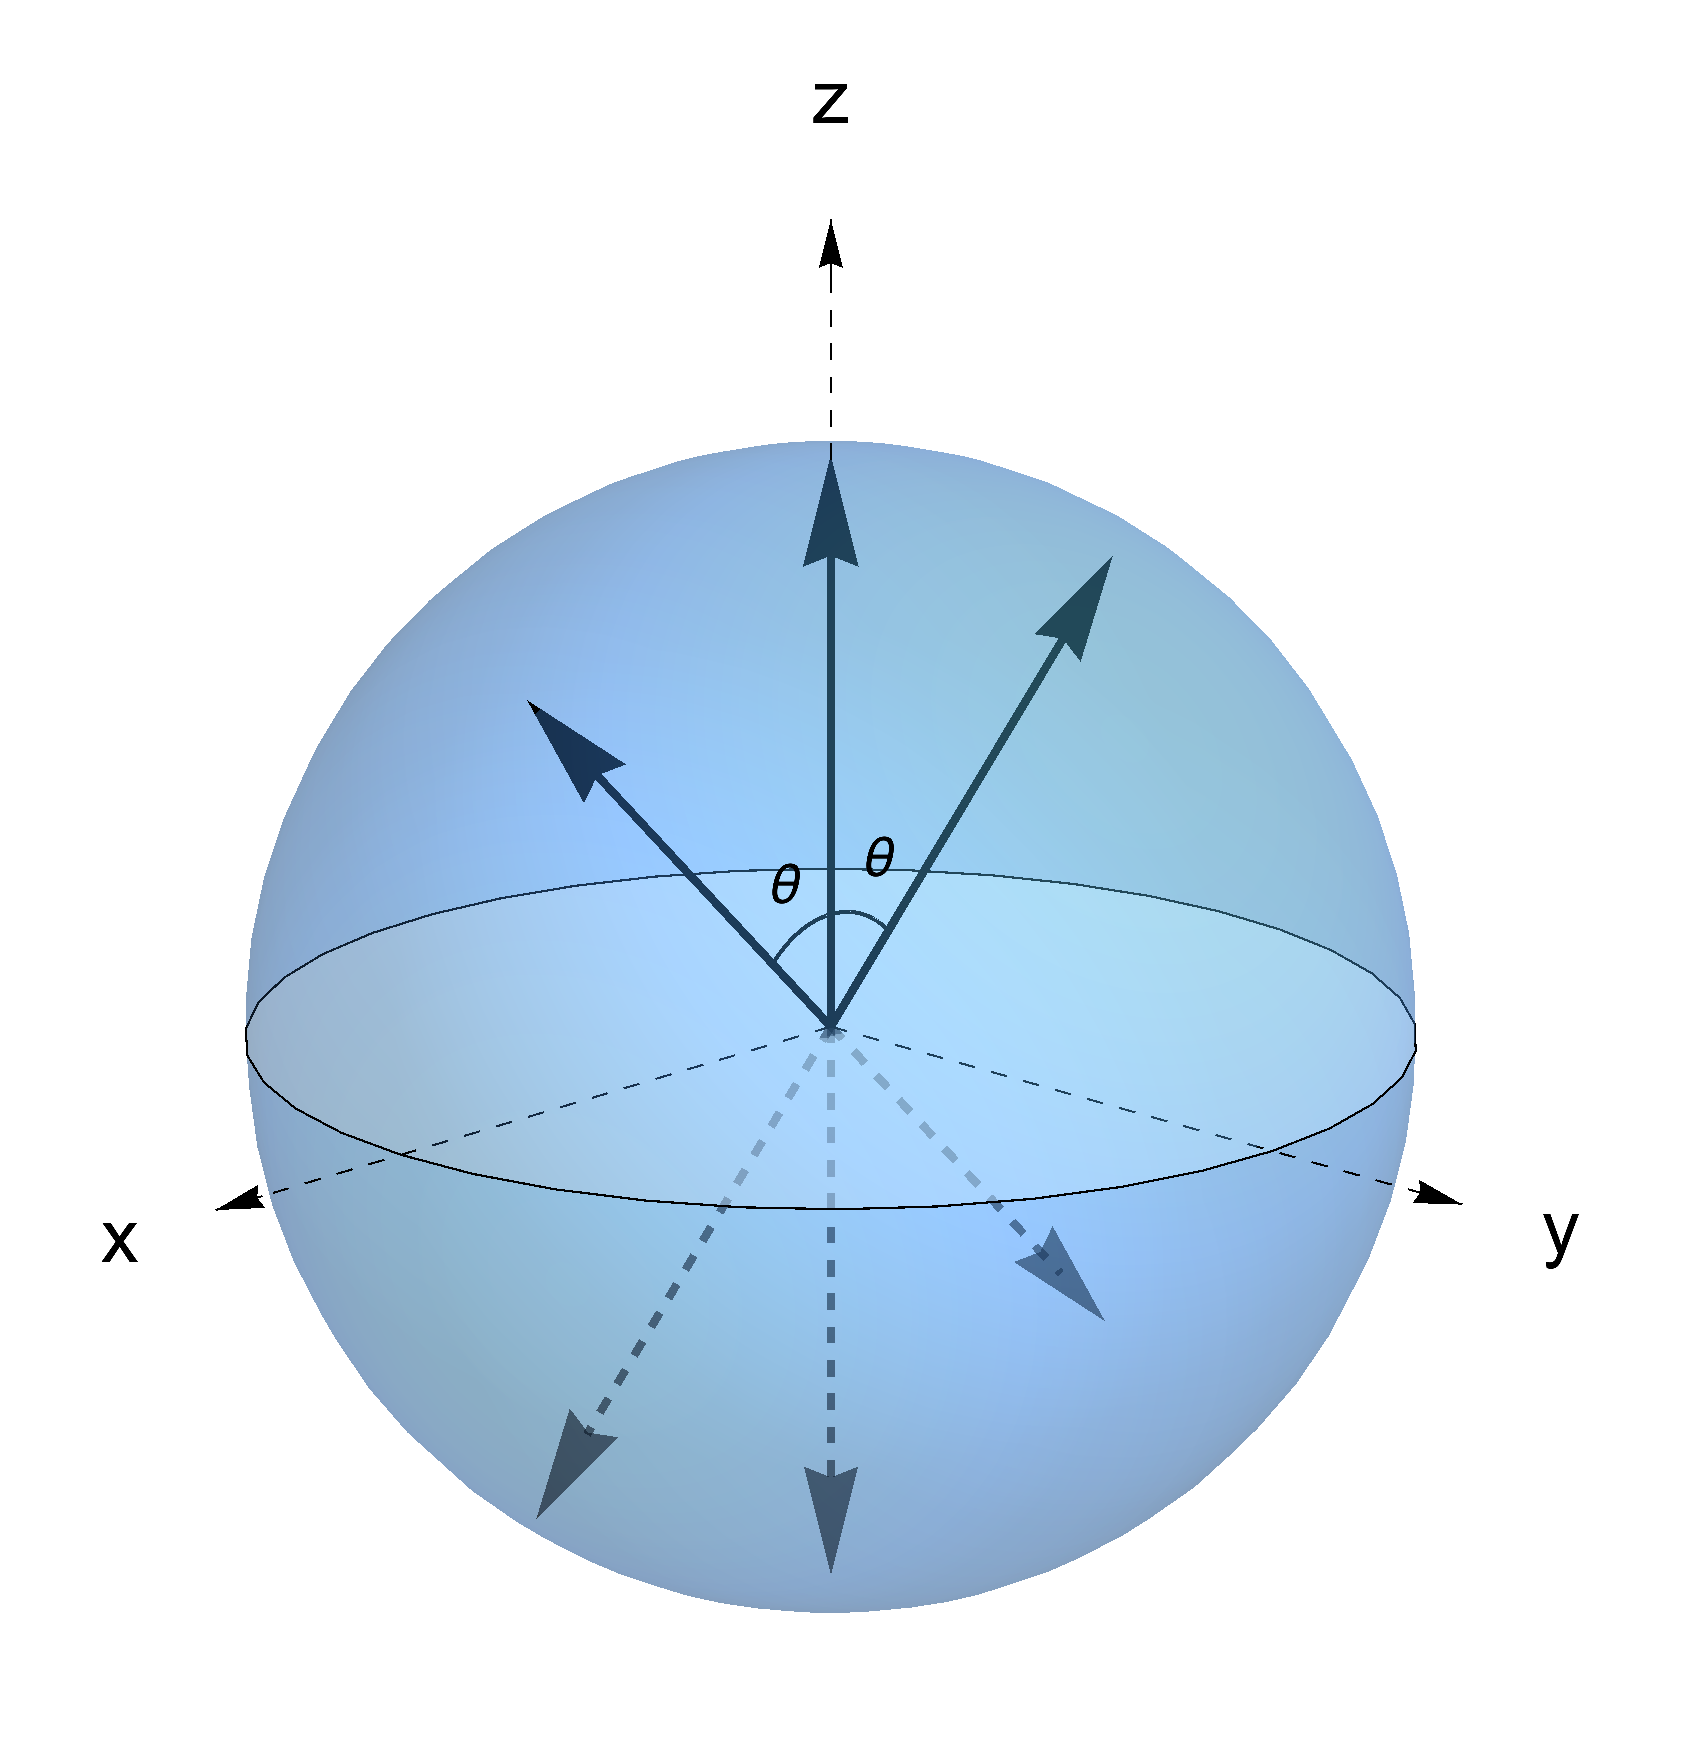
\includegraphics[width=.55\columnwidth]{mirror-symmetric-measurements.png}
            %     \caption{Measurements used to show the existence of classical, non-jointly measurable measurements. The projection on $\mathbf{z}$ and its antipodal effect are fixed, while the two other measurements vary with $0 \leq \theta \leq \pi/2$. In the upper bound, they degenerate in an $\mathbf{x}$ measurement.}
            % \label{fig:mirror-symmetric-measurements}
            % \end{figure}
            % %
            % \begin{figure}
            %     \centering
            %     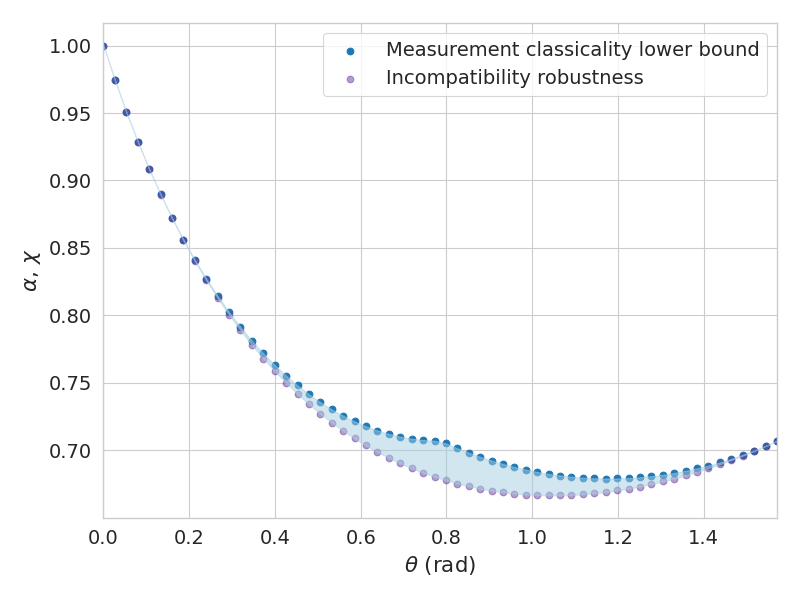
\includegraphics[width=.8\columnwidth]{incompatibility-vs-classicality.png}
            %     \caption{Incompatibility is insufficient for non-classicality in the prepare and measure scenario. For each $\theta$ (see fig. \ref{fig:mirror-symmetric-measurements}), any $\chi$ above the incompatibility robustness curve stands for an incompatible measurement set, and any $\alpha$ below the measurement classicality lower bound represents measurements that certifiedly do not generate non-classical statistics, regardless what preparations they act upon. Thenceforth, the shaded region contains incompatible albeit classical measurements.}
            % \label{fig:incompatibility-vs-classicality}
            % \end{figure}

			\begin{figure*}[t!]
				\newdimen\subfigcapmargin  \subfigcapmargin  =  -3em
				\centering
				%
				\subfigure[]{\label{fig:mirror-symmetric-measurements}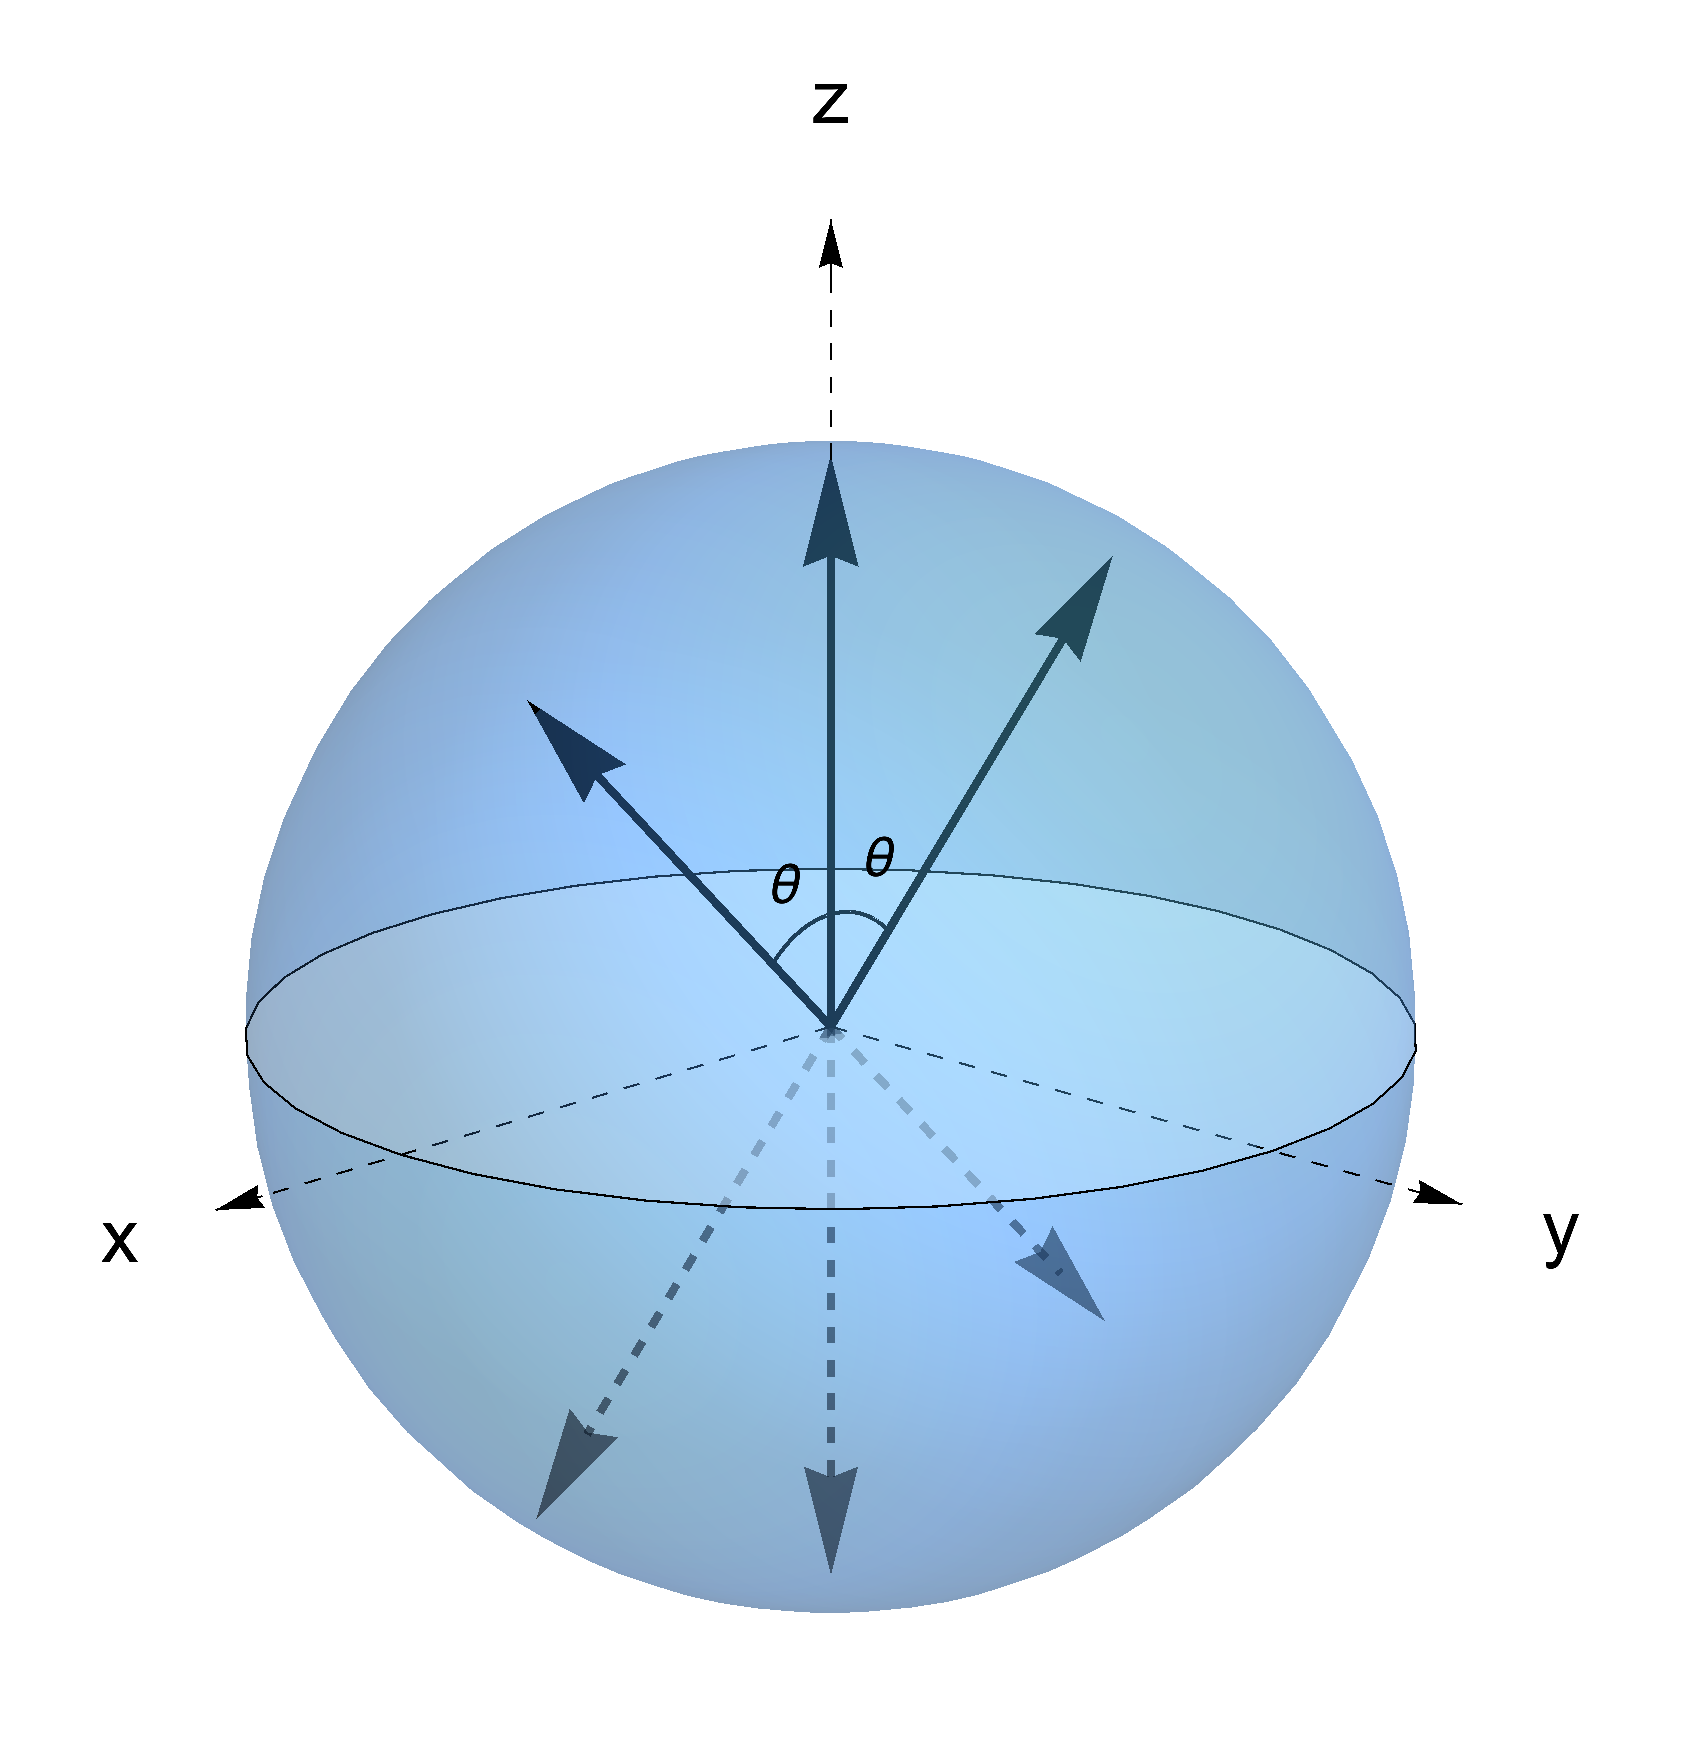
\includegraphics[width=.4\linewidth]{mirror-symmetric-measurements.png}}\hfill
				\subfigure[]{\label{fig:incompatibility-vs-classicality}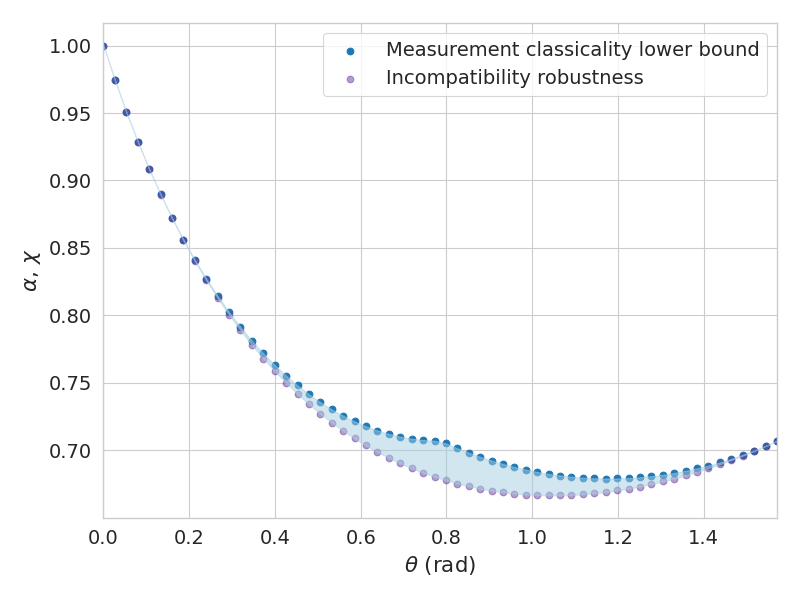
\includegraphics[width=.58\linewidth]{incompatibility-vs-classicality.png}}\hfill
				%
				\caption{Incompatibility is insufficient for non-classicality in the prepare and measure scenario. On the left, parametrized measurements used in the demonstration. The projection on $\mathbf{z}$ and its antipodal effect are fixed, while the two other measurements vary with $0 \leq \theta \leq \pi/2$. In the upper bound, they degenerate in an $\mathbf{x}$ measurement. On the right, program~\eqref{eq:measurement-classicality-projective} was applied. For each $\theta$ (see fig. \ref{fig:mirror-symmetric-measurements}), any $\chi$ above the incompatibility robustness curve stands for an incompatible measurement set, and any $\alpha$ below the measurement classicality lower bound represents measurements that certifiedly do not generate non-classical statistics, regardless what preparations they act upon. Thenceforth, the shaded region contains incompatible albeit classical measurements.}
			\end{figure*}

            Program~\eqref{eq:measurement-classicality-projective} was used to generate the upper curve in the same figure. Twenty-four probe preparations were disposed as the vertices of a rhombicuboctahedron, leading to $\eta \approx 0.86$, and the deterministic strategies were iteratively explored following the algorithm described in appendix \ref{ap:a-computational}. For each $\theta$, the obtained $\alpha$ is a lower bound on the visibility of $\mathcal{M}$ such that a classical model exists for all preparations. Specifically, anything below the classicality curve defines a measurement set which cannot generate nonclassical behaviors. The non-empty region between these two curves certifies there are plenty of incompatible measurements which are classical. Accordingly, non-joint measurability is insufficient for nonclassicality in the prepare-and-measure scenario.


        %%%%%%%%%%%%%%%%%%%%%%%%%%%
        \section{Open questions}

        Albeit the applications discussed in secs. \ref{sec:nonclassicality-activation} and \ref{sec:incompatibility-vs-classicality} rely on the projective measurements case of our criterion, their respective instances for generalized measurements are easily implementable. They do, however, incur in more demanding computational requirements, as the measurement depolarization factor $t$ can be seen as effectively lowering the insphere radius $\eta$. It could nevertheless be interesting to investigate applications of it, as for instance searching for a nonclassicality activation phenomenon valid for all POVMs.

        A second kind of activation phenomenon, emerging by adding more measuremens instead of preparations, has also been observed when the number of preparations is limited \cite{poderini_pamcriteria_2020}. Similarly to sec. \ref{sec:nonclassicality-activation}, the measurement classicality criterion derived in sec. \ref{sec:measurement-classicality} could be used to attempt on finding a more general form of this result, where all preparations are considered.

        Another interesting question is whether POVMs can be used to demonstrate nonclassicality when all PVMs fail to do so. One could approach this in the following manner. Start by selecting classical preparation sets from the results in sec. \ref{sec:nonclassicality-activation} --- which are certifiedly classical for all projective measurements. Then characterize the facets of a $(d=2, B>2, X=3,Y)$ prepare-and-measure polytope. Finally, look for a set of POVMs that, for some of those classical preparation sets, violates any of the obtained facets.

        In view of the method itself, choosing $\Phi$ as the noise model is a natural but not required choice. Different transformations, such as inscribing an ellipsis instead of a depolarized Bloch ball in $\conv{\mathcal{M}}$ (and then applying the corresponding dual map to the preparations) could lead to better computational results, and, potentially, to new insights \cite{fillettaz_algorithmic_2018}.

		The relationship of prepare-and-measure scenarios with random access coding, which was only superficially explored in sec. \ref{sec:racs} and sec. \ref{sec:nonclassicality-activation}, also deserves more exploration. Although the mapping of a RAC to a PM scenario can be trivially done, this is not enough to prove a RACs $\psuc$ is always a facet of the corresponding PM polytope. Believing that, as in the $\rac{2}{2}{1}$, this was always the case, we have further investigated this question. It turns out this is not true. In the general case, a RAC's $\psuc$ must then be some lower dimensional face of prepare-and-measure polytopes. One possible direction is to investigate whether there are subclasses of RACs with this property, of which the $\rac{2}{2}{1}$ is but one example. Another is to explore the meaning of other classes of inequalities defining PM polytopes, and if they represent other instances of information retrieval tasks.

        We believe all these suggestions are worthy of pursuit. Implementations of the programs used in this chapter could be helpful to some of these questions, and are available at a public code repository \cite{classicality_repository}.
		\chapter{Dense coding in the prepare and measure scenario}
\label{chap:pam-quantum}

    Dense coding is an astonishingly straightforward use of quantum systems to improve the transmission of classical information. In sharp contrast to Holevo's bound \cite{holevo-bound-1973}, it allows for the lossless encoding of two dits in one single qudit. Entanglement between the communicating parties is the price to pay for that. In its original formulation \cite{bennett_1992_superdense}, dense coding is a device dependent protocol: Alice's encoding operators and Bob's measurements must be fully characterized. Already hinted in sec. \ref{sec:dense-coding} is the possibility of interpreting a type of prepare and measure scenario --- the one with quantum preparations, entanglement assistance, and a single measurement --- as a physical implementation of dense coding. In return, the characterization requirements are eased, and, remarkably, interesting properties can be inferred from imposing bounds on the amount of communication and observing the behaviors. Our task in this chapter is to define this device-independent formulation of dense coding and derive some first results. Among them, we will show how to build entanglement witnesses, self-test maximally entangled states, and optimize the preparations and measurements to better perform the protocol. Stepping in the direction of more general entanglement-assisted prepare and measure scenarios, we also provide a witness in the case where more measurements are allowed.

    These results were published in \cite{moreno_pamdense_2021}, and all their proofs are provided in appendix \ref{ap:pam-quantum}.


    %%%%%%%%%%%%%%%%%%%%%%%%%%%%%%%%%%%%%%%%%%%%%%%
    \section{Semi-device-independent dense coding}
    \label{sec:sdi-dense-coding}
        In dense coding, two parties share an entangled pair and communicate via a quantum state. Quantum communication happens one-way, and the transmitted state is of the same local dimension (w.r.t. the encoding device) as the entangled pair. The task is to encode a classical message $x \in \mathcal{X} \equiv \posrange{N-1}$, and it is known that two \emph{d}its ($N = d^2$) can be perfectly recovered from one qudit of communication, for some choices of a measurement with $N$ outcomes \cite{barenco_dense_1995}.
    
        Translating to the prepare and measure lingo, we let Alice and Bob share an entangled state $\rho \in \densop{\hilb_A \otimes \hilb_B}$ as a resource. Their local dimensions, $\dim{\hilb_A} = d_A$ and $\dim{\hilb_B} = d_B$, need not be the same, but Alice's preparation must be of dimension $d_A$. To achieve quantum advantage in the dense coding task, Alice and Bob must be able to exploit the correlations available in their entangled pair. Under the circumstances, her most general strategy is to apply a local transformation $\Lambda_x : \densop{\hilb_A} \mapsto \densop{\hilb_A}$ directly on her share of $\rho$, then send it to Bob. After that,
        %
        $$
            \rho \mapsto \left( \Lambda_x \otimes \id \right)\rho \equiv \rho_x
        $$
        %
        will be in his possession. It is crucial to enforce that
        %
        $$
            \ptr{A}{\rho_x} = \ptr{A}{\rho_{x^\prime}} \quad\forall x, x^\prime ,
        $$
        %
        a condition remindful of no-signaling, for it subsumes the fact the Alice's operations, being local, cannot affect Bob's marginal state. On his end, a good selection of a quantum measurement $\mathcal{M} = \{ E_b \}_{b=0}^{k-1}$ may provide advantage (over classical encodings) in the task of recovering her choice of $x$. Naturally, $\sum_b E_b = \id$, and each $E_b$ is a positive semidefinite operator acting on $\hilb_A \otimes \hilb_B$, which means to say he measures on both his and her transformed share of $\rho$. Summing it up, dense coding behaves in $\mathcal{Q}^\rho_{d_A,d_A^2,d_A^2,1}$, but we will also discuss some further generalizations.
        
        Many rounds of this protocols allow Alice and Bob to collectively infer the behavior
        %
        $$
            \mathbf{p} = \{ \condprob{b}{x} \}_{b,x} = \{ \tr{\rho_x E_b } \}_{b,x} .
        $$
        %
        From the behavior, we can assess their performance in the protocol. To that end, we assume that her choices of $x$ are equiprobable in $\mathcal{X}$ and define the figure of merit as
        %
        \begin{equation}
            p_{\text{suc}} = \frac{1}{N} \sum_{x=0}^{N-1} \condprob{b=x}{x} .
            \label{eq:psuc-dense-coding}
        \end{equation}
        %
        This is the very same average success probability discussed under the random access coding protocols of sec. \ref{sec:racs}, except that we now deal with a single measurement on Bob's side. Differently from the usual dense coding formulation --- which requires knowledge on the exact preparations and measurements employed ---, computing $p_{\text{suc}}$ relies solely on observational data. It is thus a device-independent figure of merit, completing our device-independent formulation of the dense coding protocol.
        
    %%%%%%%%%%%%%%%%%%%%%%%%%%%%%%%%%%%%%%%%%%%%%%%%%%%%%%%%
    \section{Witnessing and self-testing entanglement}

        Understanding the relationships between some figure of merit and the underlying resources is a commonplace question in device-independent scenarios. Important ones for the prepare and measure formulation of dense coding are which bounds the amount of entanglement in $\rho$ or its local dimensions imply on $\psuc$, and whether violating them witness or even self-tests some property of $\rho$. 
    
        Brunner et al. \cite{brunner_dimension_2013} considered similar questions in the quantum state discrimination scenario. Similarly to ours, their scenario allowed for a single measurement, and their figure of merit was equivalent to $\psuc$. However, the devices were independent, and their investigation focused on what could be inferred about quantum versus classical preparations. In chap. \ref{chap:pam}'s terminology, they were mostly interested in analyzing $\psuc$ in $\mathcal{C}_{d<N,N,N,1}$ against $\mathcal{Q}_{d<N,N,N,1}$. Interestingly, they found out both classical and quantum bounds for $\psuc$ are equal to $d_A / N$. Therefore, while that success probability can be used as a dimension witness, it cannot witness the type of preparations.
        
        Our first result generalizes theirs in the following way
        %
        \begin{restatable}[Schmidt number witness]{res}{schmidtnumber}
            Let $\rho$ be a shared resource with Schmidt number $s$ and local dimension $d_A$ on Alice's side. If she chooses one out of $N$ preparations, and Bob performs a single measurement with $N$ outcomes on the joint state, then
            %
            \begin{equation}
                \psuc \leq \min \left( \frac{d_A s}{N}, 1 \right) .
                \label{eq:result-1}
            \end{equation}
            %
            When $N \geq d_A s$, the bound is tight.
            \label{res:1}
            \label{res:schmidt-number-witness}
        \end{restatable}
        %
        Separable states ($s=1$) thus recover the bound $\psuc \leq d_A / N$ from \cite{brunner_dimension_2013}. For this reason, whenever the transmitted state's dimension is knowingly $d_A$, a $\psuc > d_A / N$ witness entanglement. Because only local operations are used to prepare the $\rho_x$, and those cannot increase $s$, any $\psuc > d_A s / N$ unambiguously certifies that $\rho \notin S_s$, so providing a lower bound on its Schmidt number.
        
        A particular instance of ineq. \ref{eq:result-1} can also be used for self-testing maximally entangled states.
        %
        \begin{restatable}[Self-testing maximally entangled states]{res}{selftest}
            In dense coding instances ($N=d_A^2$) of the prepare and measure scenario with $s=d_A$, saturation of ineq. \ref{eq:result-1} certifies, up to a local unitary transformation, that the shared state $\rho$ is maximally entangled.
            \label{res:self-testing-maximally-entangled}
        \end{restatable}
        
        Interestingly, this has implications for quantum key distribution protocols in the prepare and measure dense coding scenario. Suppose Alice does not actually share a maximally entangled pair with Bob, but rather with a third, malicious party that wants to eavesdrop on their communication. Let us suitably call her Eve. Apart from sharing a maximally entangled pair $\rho_{AE}$ with Alice, she intercepts Alice's communication of her share of $\rho_x$. From result \ref{res:self-testing-maximally-entangled}, she reads out $x$ with $\psuc = 1$, thus perfectly learning Alice's message. Because, at the end of the day, it will be Alice and Bob who share data to infer their $\psuc$, Eve must share a second maximally entangled pair $\rho_{EB}$ with Bob, which she exploits to reencode $x$ and transmit to Bob. In this way, Alice and Bob's $\psuc$ will saturate, tricking them into believing they share a maximally entangled pair. As Eve succeeds in eavesdropping without being detected, the prepare and measure dense coding protocol is not cryptographically secure.
        
        Historically, dense coding was introduced as a perfect encoding protocol. Relaxing this condition, by letting $\psuc < 1$, can shine more light on the role of entanglement assistance. Sharing pure entangled states, as the following result shows, is always advantageous over having only classical correlations (in the form of separable states).
        %
        \begin{restatable}[Pure states quantum advantage]{res}{purestates}
            Sharing a pure entangled state, which we write in the Schmidt decomposition $\ket{\psi} = \sum_{i = 0}^{s-1} \eta_i \ket{i} \otimes \ket{i}$, the best probability of success in the encoding of $N = d_A^2$ dits is lower bounded as
            %
            $$
                \psuc \geq \min \left( \frac{1 + \Gamma}{d_A}, \,1 \right),
            $$
            %
            where $\Gamma \equiv \sum_{i \neq j} \eta_i \eta_j \geq 0$.
        \label{res:pure-states-advantage}
        \end{restatable}
        
        From result \ref{res:1}, $N = d_A^2$ with $\rho \in \text{SEP}$ implies that $\psuc \leq 1 / d_A$, and as an entangled state is such that $\Gamma > 0$, all pure entangled states provide quantum advantage in the dense coding protocol.
        
        As a corollary, we have an amusing alternative proof to the possibility of perfectly encoding two dits in a qudit: a maximally entangled state has all $\eta_i = 1 / \sqrt{d_A}$ (c.f. sec. \ref{sec:states}), by which $\Gamma = d_A - 1$, thus $\psuc = 1$.
        
        Apropos of mixed states, a similar relation holds. Setting $d_A = d_B = d$ and making use of the singlet fraction $\zeta(\rho)$, which, in a loose sense, measures how much of a maximally entangled state is in $\rho$ (sec. \ref{sec:states}), it is true that
        %
        \begin{restatable}[Singlet fraction bound]{res}{singletfraction}
            The best probability of success achievable with a resource $\rho$ is lower bounded as
           \begin{equation}
                \psuc \geq \zeta(\rho) .
                \label{eq:psuc-singlet-fraction}
            \end{equation}
        \label{res:singlet-fraction-bound}
        \end{restatable}

        Interestingly, this fact closely links our witness to \emph{faithful entangled states}. These are defined to be those states whose entanglement can be certified by a fidelity-based witness, and it was recently proven that a state is faithful if and only if its singlet fraction is greater than $1/d$ \cite{guhne_faithful_2021}. Eq. \ref{eq:psuc-singlet-fraction} hence implies that any $\psuc > 1/d$ certifies $\rho$ is faithful. 
 
        As another application of this same result, consider an isotropic state (sec. \ref{sec:states})
        %
        $$
            \chi(\alpha) = \alpha \ketbra{\Phi^+}{\Phi^+} + (1 - \alpha) \frac{\id}{d^2} ,
        $$
        %
        which is separable only in the range $\alpha \leq \frac{1}{d + 1}$. Its singlet fraction is
        %
        $$
            \zeta\left[ \chi(\alpha) \right] = \alpha + \frac{1 - \alpha}{d^2} ,
        $$
        %
        and monotonically decreases with decreasing $\alpha$. As
        %
        $$
            \zeta \left[ \chi \left( \frac{1}{d + 1} \right) \right] = \frac{1}{d}
        $$
        %
        is the classical bound for $\psuc$ (result \ref{res:1}), it follows that $\psuc \geq \zeta(\rho)$ can witness entanglement for all isotropic states.        

        As pointed in sec. \ref{sec:states}, isotropic states are a common benchmark for quantum informational protocols. In particular, there are entanglement witnesses in the Bell nonlocality and quantum steering scenario that can certify a $\chi(\alpha)$ is entangled from some critical visibility $\alpha_{\text{crit}}$ upwards. Before contrasting them to our result, it is important to justify whether the comparison is fair. In the case of Bell nonlocality, it is not. Any prepare and measure scenario allows for communication, and all our witnesses rely on local dimension bounds, thus being only semi-device-independent. Contrastingly, Bell nonlocality is built on a causal structure with no direct relations between the parties, and is fully device-independent. Therefore, we expect any witness in this scenario to perform more poorly. The answer for quantum steering is not so clear-cut. While it also forbids communication, it does rely on local tomography for one of the parties. This presupposes full characterization of one measurement device, and hence also knowledge on the state dimension. Nevertheless, as made evident in fig. \ref{fig:isotropic-witness} it does perform rather badly in comparison to our singlet fraction witness. The tests used were the Collins-Gisin-Linden-Massar-Popescu (CGLMP) inequality \cite{collins_cglmp_2002} and Wiseman et al.'s truncated harmonic series relation \cite{wiseman_2007_steering} (also stated in sec. \ref{sec:states}). CGLMP is not proven optimal for isotropic states, and in fact, for specific dimensions, better ones are known (e.g., \cite{divianszky_qutritwitness_2017}). On the other hand, the steering witness employed is only optimal for projective measurements. The case for POVMs is not so clear, and may lead to better witnesses \cite{nguyen_somemeasurements_2020}.
        
        \begin{figure}
            \centering
            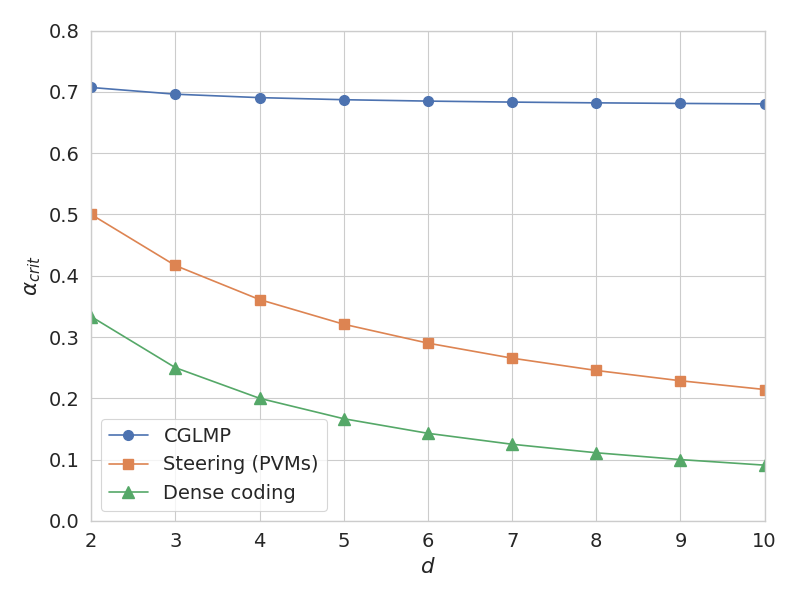
\includegraphics[width=.65\columnwidth]{isotropic-witness.png}
            \caption{Comparison between witness \ref{eq:psuc-singlet-fraction} to the CGLMP Bell inequality witness \cite{collins_cglmp_2002} and Wiseman et al.'s steering witness \cite{wiseman_2007_steering} for isotropic states (eq.~\eqref{eq:isotropic-states}). With a dimension assumption, the prepare and measure dense coding scenario can witness all entangled isotropic states. See the main text for a discussion on the fairness of this comparison.}
        \label{fig:isotropic-witness}
        \end{figure}
        
        Taking first step towards the study of more general entanglement assisted prepare and measure scenarios, we extend another result from the state discrimination task studied in \cite{brunner_dimension_2013}. In it, the authors allowed there to be $Y = N (N-1)/2$ dichotomic measurement choices, where $N$ is the number of preparations. Each measurement is labeled as the pair $(x, x^\prime)$, where $x > x^\prime$ with $x, x^\prime \in \posrange{N-1}$, and the behaviors now have elements $\condprob{b}{x,y}$. Their result states that, for uncorrelated parties, the expression
        %
        $$
            V_N \equiv \sum_{x > x^\prime} \abs{ \condprob{b=1}{x, (x, x^\prime)} - \condprob{b=1}{x^\prime, (x, x^\prime)} }^2 \leq \frac{N^2}{2} \left( 1 - \frac{1}{\min(d_A,N)} \right)
        $$
        %
        is a quantum dimension witness for any communication dimension $d_A < N$, and can also distinguish between quantum and classical systems (in the sense of pair-wise mutually commuting preparations, explained in sec. \ref{sec:quantum-behaviors}) for any $N$ which is not a multiple of $d$. By allowing for an entangled resource of Schmidt number $s$ between the parties, we found the following generalization.
        
        \begin{restatable}[Multiple measurements witness]{res}{moremeasurements}
            Given a shared bipartite resource with Schmidt number $s$, a prepare and measure scenario with $N$ $d_A$-dimensional preparations labeled by $x \in \posrange{N-1}$, and $N (N-1)/2$ dichotomic measurements labeled as $(x, x^\prime)$ for $x > x^\prime$ is such that
            %
            \begin{align*}
                V_N &\equiv \sum_{x > x^\prime} \abs{ \condprob{b=1}{x, (x, x^\prime)} - \condprob{b=1}{x^\prime, (x, x^\prime)} }^2 \\
                &\qquad\qquad\leq \frac{N^2}{2} \left( 1 - \frac{1}{\min(d_A s,N)} \right) .
            \end{align*}
            %
            If $s = d_A$, and $N < d_A^2$ or $N$ is an integer multiple of $d_A^2$, the inequality is tight.
            \label{res:more-measurements}
        \end{restatable}
        
        For fixed $N$ and $d_A$, $V_N$ can witness whether $\rho \in S_s$ or not.
    

    %%%%%%%%%%%%%%%%%%%%%%%%%%%%%%%%%%%%%%%%%%%%%%%%%%%%%%%%%%
    \section{Optimizing the dense coding probability of success}
    \label{sec:pam-quantum-optimization}

        Up until now, we have focused on what can be inferred about $\rho$ from the observable statistics. In practice, $\rho$ is sometimes treated as a resource to be consumed in the protocol, and it may be of interest to obtain the preparations $\rho_x$ and measurement $\mathcal{M} = \{ E_b \}$ that make the best use of it to achieve the largest $\psuc$. More formally, we are interested in solving
        %
        \begin{subequations}
            \begin{alignat}{2}
                &\text{given}    &\quad & \rho \\
                &\underset{\mathcal{M}, \Lambda_x}{\text{max.}}   &	  & \frac{1}{N} \sum_0^{N-1} \trb{ E_x \left( \Lambda_x \otimes \id \right) \rho} \label{eq:obj-func-cptp}\\
                &\text{s.t.}    &      & \Lambda_x \in \text{CPTP}, \quad\forall x \\
                &				   &	  & E_x \succeq 0, \quad\forall x \\
                &                  &      & \sum E_x = \id .
            \end{alignat}
            \label{eq:psuc-base-program}
        \end{subequations}
        %
        For an arbitrary $\rho$, this is a daunting task to approach analytically. Even numerically, the objective function is nonlinear, and optimizing over CPTP constraints is not directly a recognizable constraint. This lends little hope to the problem of efficiently finding global maxima. It is nevertheless possible to formulate an alternated semidefinite optimization procedure (also called \emph{see-saw} optimization) that solves to local extrema.

        Using channel-state duality (eqs.~\eqref{eq:channel-to-state} and \eqref{eq:state-to-channel}), the CPTP map $\Lambda_x$ can be cast as a bipartite state, for which the constraints of positivity and unit-trace are amenable to semidefinite programming. To see how, let $L_x \in \densop{\hilb_A \otimes \hilb_{A^\prime}}$ be the state dual to the channel $\Lambda_x : \densop{\hilb_A} \mapsto \densop{\hilb_{A^\prime}}$, where the superscript in $\hilb_{A^\prime}$ was added for ease of reading. Using $L_x$, the action of $\Lambda_x \otimes \id_B$ on the shared state $\rho$ is equivalent to $\ptrb{A}{(L_x \otimes \id_B) (\rho^{\intercal_A} \otimes \id_{A^\prime})} \in \densop{\hilb_{A^\prime} \otimes \hilb_B}$, where we only partially transpose $\rho$ because $\Lambda_x$ is local to Alice. Bob's measurement effects, $E_x$, will then act on $\densop{\hilb_{A^\prime} \otimes \hilb_{B}}$. Putting this into our objective function (eq.~\ref{eq:obj-func-cptp}), dropping the partial trace in favor of the trace, and completing $E_x$ to $\id_A \otimes E_x$ makes program~\eqref{eq:psuc-base-program} equivalent to
        %
        \begin{subequations}
            \begin{alignat}{2}
                &\text{given}    &\quad & \rho \\
                &\underset{\mathcal{M}, L_x}{\text{max.}}   &	  & \frac{1}{N} \sum_0^{N-1} \trb{ \left( L_x \otimes \id_B \right) \left(\rho^{\intercal_A} \otimes \id_{A^\prime} \right) \left( \id_A \otimes E_x \right)} \\
                &\text{s.t.}    &     & L_x \succeq 0, \quad\forall x \label{eq:constr-cp-map}\\
                &			    &	  & \ptr{A^\prime}{L_x} = \id_{A}, \quad\forall x \label{eq:constr-trace-preserving}\\
                &				&	  & E_x \succeq 0, \quad\forall x \\
                &               &     & \sum E_x = \id .
            \end{alignat}
            \label{eq:dense-coding-optimization}
        \end{subequations}
        %
        %where $^{\intercal_A}$ is a partial transposition on the $A$ system and the $L_x \in \mathcal{L} (\hilb_A \otimes \hilb_B)$ correspond to the preparations $\Lambda_x$. The constraints are all linear matrix inequalities (\ref{sec:sdp}), but the objective function is still nonlinear.
		These constraints are all linear matrix inequalities, and eqs.~\eqref{eq:constr-cp-map} and \eqref{eq:constr-trace-preserving} are in there to guarantee $L_x$ is completely positive and trace-preserving. We are closer to an SDP, but the objective function is still nonlinear. To circumvent that, we sample an initial measurement $\mathcal{M}^0$, fix it for the time being, and run program \ref{eq:dense-coding-optimization} only on the $L_x$ variables. The objective function is then clearly linear, and the last two constraints shall be removed. With the optimal (w.r.t. $\mathcal{M}_0$) $L_x$ from this first iteration, which we call $L_x^1$, fixed, optimizing over the measurements is also a semidefinite program. In this second step, the first two constraints may be left out, and we call its result $\mathcal{M}^1$. Together, $\mathcal{M}^1$ and $L_x^1$ are the result of the first iteration, and provide a lower bound on the best $\psuc$. After $N$ iterations, convergence can be tested through some heuristic criterion, such as checking whether $\psuc \left( \mathcal{M}^N, L_x^N \right) - \psuc \left( \mathcal{M}^{N-1}, L_x^{N-1} \right) \approx 0$. Different samples of $\mathcal{M}_0$ can lead to distinct results, and no formal guarantee of global extremality is provided by this procedure. Nonetheless, this is a computationally inexpensive procedure, thus running it for several initial samples and taking the best solution may provide numerical evidence of optimality. And, of course, one might as well start by sampling a $L_x^0$ and inverting the order of the programs.

        To see it in action, consider the Werner states (sec. \ref{sec:states}) parameterized as
        %
        \begin{equation}
            \rho_W ( \alpha ) = \frac{\id - \alpha S}{d^2 - \alpha d} ,
            \label{eq:werner-dense-coding}
        \end{equation}
        %
        where $d$ is the local dimension, $-1 \leq \alpha \leq 1$, and $S = \sum_{i,j=0}^{d-1} \ketbra{ij}{ji}$ is the swap operator. For $N = d^2$ preparations and a measurement with $N$ outcomes, we optimize the dense coding probability of success for $d \in \{2, \ldots, 5\}$ and a linear range over $\alpha$. Results are shown in fig. \ref{fig:werner-dense-coding-psuc}. All values of $\alpha \lesssim (d-1)/d$ saturate the classical (i.e., $s=1$) bound of $1/d$ from result \ref{res:1}, and every larger $\alpha$ violates it. In the inset, a comparison of $\psuc$ with the classical bound $1/d$, for $\alpha = 1$, suggests that Werner states of larger dimension provide smaller quantum advantages in dense coding.

		% \begin{figure*}[t!]
		% 	\newdimen\subfigcapmargin  \subfigcapmargin  =  -3em
		% 	\centering
		% 	%
		% 	\subfigure[]{\label{fig:werner-opt}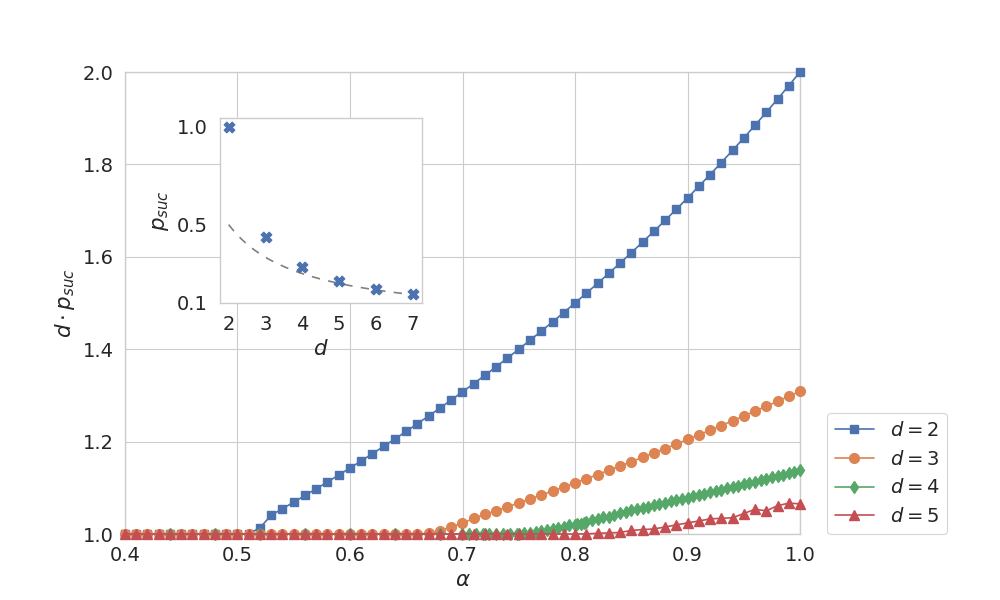
\includegraphics[width=.58\linewidth]{werner-opt.png}}\hfill
		% 	\subfigure[]{\label{fig:werner-opt-dims}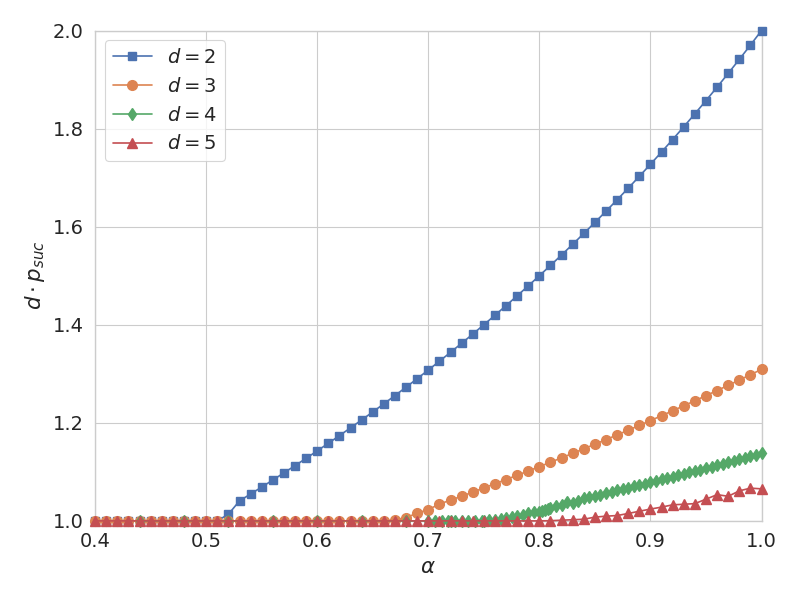
\includegraphics[width=.4\linewidth]{werner-opt-dims.png}}\hfill
		% 	%
        %     \caption{Optimal $\psuc$'s obtained for Werner states~\eqref{eq:werner-dense-coding} with the alternated optimization procedure over program~\eqref{eq:dense-coding-optimization}. Squares, circles, rhombuses and triangles correspond to $d = 2, 3, 4$ and $5$, respectively. Values are reescaled so that all classical bounds correspond to $1$. The inset shows $\psuc$ for $\alpha = 1$ (crosses) against the classical bound of $1/d$ in dimensions $2$ up to $7$.}
        % \label{fig:werner-dense-coding-psuc}
		% \end{figure*}
        
        \begin{figure}
            \centering
            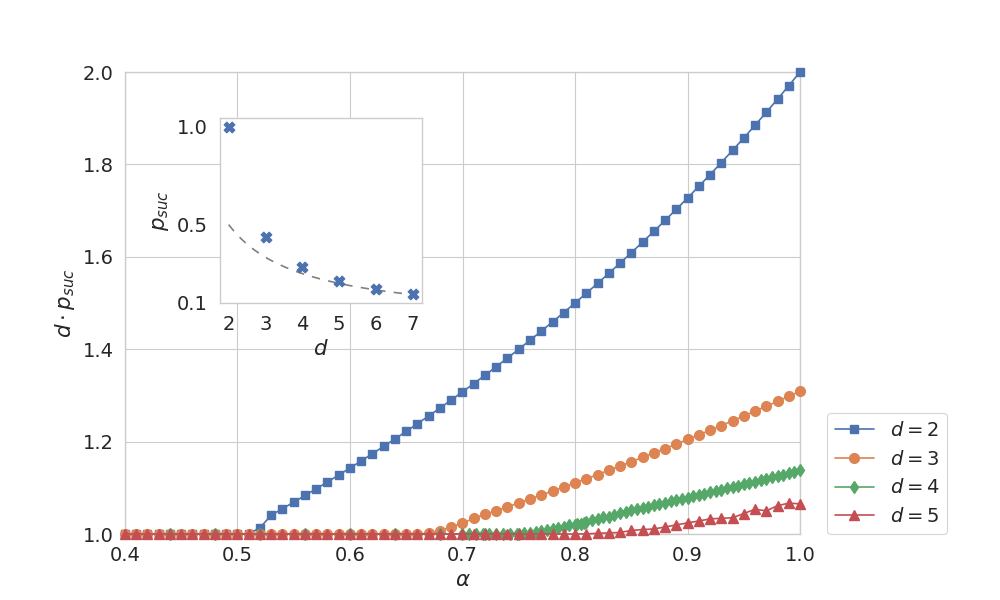
\includegraphics[width=.9\columnwidth]{werner-opt.png}
            \caption{Optimal $\psuc$'s obtained for Werner states~\eqref{eq:werner-dense-coding} with the alternated optimization procedure over program~\eqref{eq:dense-coding-optimization}. Squares, circles, rhombuses and triangles correspond to $d = 2, 3, 4$ and $5$, respectively. Values are reescaled so that all classical bounds correspond to $1$. The inset shows $\psuc$ for $\alpha = 1$ (crosses) against the classical bound of $1/d$ (dashed curve) in dimensions $2$ up to $7$.}
        \label{fig:werner-dense-coding-psuc}
        \end{figure}

    
    %%%%%%%%%%%%%%%%%%%%%%%%%%%%%%%%%%%%%%%%%%%%%%%%
    \section{Open questions}

    Regarding device-independent dense coding, an interesting possibility is to generalize its definition by allowing Alice's local dimension $d_A$ to be larger than the actual communicated qudit, i.e., to let $\Lambda_x : \densop{d_A} \mapsto \densop{d}$, with $d < d_A$. First discussions on that situation were recently started in \cite{nayak_rigidity_2020,tavakoli_eapam_2021}. As noted in \cite{tavakoli_eapam_2021}, in that case a road worth taking is to investigate if there are witnesses that do not depend on $d_A$, but only on the communicated state dimension. Application-wise, while the see-saw optimization procedure is reasonably efficient, it would be useful to better understand what types of guarantees regarding global optimality are possible to provide. Secondly, one could think of a conceptual explanation as to why higher dimensional Werner states are increasingly worse in outperforming the classical bound on $\psuc$, and whether this trend is also present in other classes of entangled states.

    General entanglement assisted prepare and measure scenarios --- and especially the one with quantum preparations --- are little explored in the literature. Most results hitherto presented are only valid for the $Y=1$ case, which is of special interest but begs for generalizations. Result \ref{res:more-measurements} is a small step in that direction. Simultaneously to our results, Tavakoli et al. provided important results on the same theme \cite{tavakoli_eapam_2021}, but much is still to be done.

    Below result \ref{res:self-testing-maximally-entangled}, we discussed how an eavesdropper could intercept Alice's communication while still tricking she and Bob into believing they share a maximally entangled resource. One interest in studying $Y > 1$ witnesses is that they may provide cryptographically secure tests. To see how, consider a BB84-like protocol \cite{bb84} where Alice, before sending her qubit, randomly chooses whether to apply a $\sigma_x$ gate to it. Up to an unmeasurable global phase, $\left( \ket{\Phi^+}, \ket{\Phi^-}, \ket{\Psi^+}, \ket{\Psi^-} \right) \overset{\sigma_x}{\longmapsto} ( \ket{\Psi^+}, \ket{\Psi^-}, \ket{\Phi^+}, \ket{\Phi^-})$. An eavesdropper sharing the entangled resource with Alice and measuring in the Bell basis would correctly get $x=0$ in the first situation, but wrongly guess $x=2$ in the latter. She could try switching to a $\sigma_x$-transformed Bell measurement, but without information on Alice's decision, this would be unhelpful. Worse than that, after mistaking $x$, she would send the wrong repreparation to Bob. During the whole protocol, Bob must also be blind to Alice's choice. Let us further suppose that he can choose between a standard Bell measurement or a $\sigma_x$-transformed one and that, to make ends meet, Alice sends $M + \delta$ qubits, where $M$ is the intended key size. Afterwards, Alice publicly announces the choices of $x$ and $\sigma_x$ she made on the extra $\delta$ messages. In all rounds when Bob made the correct decision on his measurements, his result should be perfectly correlated with Alice's encoding. If he observes some of them are not, he will know Eve eavesdropped. While this example is device dependent, it is of interest to find some witness for $Y=2$ that can device-independently guarantee security in a similar protocol, or prove there is none.
	% \include{postext/final_remarks}
	
	\begin{appendices}
		\chapter{Computational details for chap. \ref{chap:pam-classical}}
\label{ap:a}
\label{ap:a-computational}
		\chapter{Proofs for chap. \ref{chap:pam-quantum}}
\label{ap:pam-quantum}

Proofs for all results in chap. \ref{chap:pam-quantum} are hereby provided. To aid in their understanding, we begin by reviewing some useful results.

\section{Mathematical tools}
\label{sec:ap-a-mathematical-tools}

    Generalized Gell-Mann matrices (sec. \ref{sec:gell-mann}) are not the only useful choice of basis for $\mathcal{L}(\hilbd{d})$. Another possibility, the \emph{Weyl operator basis} \cite{bertlmann_2008_bloch} is composed of \emph{discrete Weyl operators} which will be essential for the upcoming proofs. They are defined as
    %
    \begin{equation}
        W_{x_1 x_2}^d = \sum_{m = 0}^{d-1} e^{\nicefrac{2 \pi i x_1 m}{d}} \ketbra{m \oplus_d x_2}{m} ,
        \label{eq:weyl-operators}
    \end{equation}
    %
    where $\oplus_d$ is shorthand for a modulo $d$ sum, and $x_1, x_2 \in \{0, \ldots, d-1 \}$. The result of applying $W_{x_1 x_2}$ to some basis vector $\ket{j}$ can be interpreted as a displacement to level $\ket{j \oplus_d x_2}$ together with the inclusion of a phase $e^{\nicefrac{2 \pi i x_1 j}{d}}$. If the specific values of $x_1$ and $x_2$ are unimportant, we will label $W$ simply with $x$, and we may also omit $d$. When $x_1$ and $x_2$ running on different ranges (as will be used in the proof of result \ref{res:schmidt-number-witness}), we will call $W$ \emph{generalized} Weyl operators. But, for now, let us stick to the usual ones.

    Weyl operators have been useful at least since 1993, when they were used by Bennett et al. to devise a $d$-dimensional quantum state teleportation protocol \cite{bennett_1993_teleporting}. Much of their worthiness come from properties such as unitarity ($W_x W_x^\dagger = W_x^\dagger W_x = \id$, as can be verified by direct calculation) and orthonormality: $\tr{W_{x}^\dagger W_{y}} = d \delta_{x, y}$. Proofs can be found in \cite{bertlmann_2008_bloch}, appendix A.3, and in sec. 4.1.2 of \cite{watrous_book_2018}, presented among other interesting properties.

    Every vector $\ket{\psi} \in \hilbd{d} \otimes \hilbd{d}$ can be obtained from a maximally entangled state, such as $\ket{\Phi^+} = \frac{1}{\sqrt{d}} \sum_{j=0}^{d-1} \ket{j} \otimes \ket{j}$, by means of a \emph{unique} transformation $L_{\ket{\psi}} \otimes \id$, acting trivially on the second subsystem. Importantly, $\ket{\psi}$ is maximally entangled if and only if $L_{\ket{\psi}}$ is unitary \cite{vollbrecht_twoqubits_2000}. From the uniqueness of the $L_{\ket{\psi}} \otimes \id$, then, there are as many orthogonal maximally entangled states as the dimension of the unitary group, i.e., $d^2$. Having the $d^2$ orthonormal unitaries $W_{x_1 x_2}$ at hand, it is then true that
    %
    \begin{equation}
        \big\{ (W_{x_1 x_2} \otimes \id) \ket{\Phi^+} \big\} \equiv \big\{ \ket{\Phi_{x_1 x_2}} \big\}, \quad \forall x_1, x_2 \in \{0, \ldots, d-1\}
        \label{eq:weyl-states}
    \end{equation}
    %
    are maximally entangled and orthogonal preparations. In the prepare and measure dense coding scenario, Alice and Bob share a resource $\rho$ that she locally transforms to prepare $\rho_x = (\Lambda_x \otimes \id) \rho$. This is precisely the structure above. Furthermore, orthogonal states are perfectly distinguishable, and we thence should expect them to be good candidates for optimal performance in prepare and measure protocols.

    With poorly chosen measurements, good preparations are worthless. The $d^2$-outcome measurement
    %
    \begin{equation}
        \mathcal{M}^W = \{ \ketbra{\Phi_{x_1 x_2}}{\Phi_{x_1 x_2}} \}_{x_1, x_2 = 0}^{d-1} \equiv \{ M_x^W \},
        \label{eq:weyl-measurements}
    \end{equation}
    %
    whose effects project precisely in these maximally entangled vectors, will turn useful. To be sure it is well-defined, notice that each of its effects are obviously PSD and, as they are normalized and form a basis, $\sum_{x_1, x_2 = 0}^{d - 1} \ketbra{\Phi_{x_1 x_2}}{\Phi_{x_1 x_2}} = \id$.

    \ornamentbreak
    We end this section with three further results.

    % Outcome probability upper bound.
    \begin{lemma}[Outcome probability upper bound]
        When $\rho$ is a density operator and $M$ is a measurement effect, $tr(\rho M) \leq tr(M)$.
        \label{lem:outcome-upper-bound}
    \end{lemma}
    \begin{proof}
        $M$ is PSD, thus all its eigenvalues are nonnegative and it has a spectral decomposition. Let $M = \sum_i m_i \ketbra{m_i}{m_i}$ be it, and order the eigenvalues as $m_1 \geq \ldots \geq m_d$. Notice, also, that $\rho = \sum_i p_i \ketbra{p_i}{p_i}$, where the $p_i$ form a probability distribution. Now write 
        $$
            \text{tr}(\rho M) = \sum_{i} p_i \sum_j m_j \braket{p_i}{m_j}^2 .
        $$
        If $\rho = \ketbra{m_1}{m_1}$, then, $\text{tr}(\rho M) = m_1 \leq\text{tr}(M)$. It is now left to prove this choice leads to a maximum of $\text{tr}(\rho M)$. That is indeed the case because, as $m_1$ is a largest eigenvalue, any convex combination of the $m_i$ is at most as large as $m_1$.
    \end{proof}

    % Orthogonal states
    \begin{lemma}
        If $d^2$ quantum states $\{ \rho_x \}_{x=1}^{d^2}$, where each $\rho_x \in \hilbd{d} \otimes \hilbd{d}$, do not overlap (i.e., $\tr{\rho_x \rho_y} = 0, \,\forall x \neq y$), they must be pure.
        \label{lem:overlap}
    \end{lemma}
    \begin{proof}
        Each of the $\rho_x$ has a spectral decomposition $\rho_x = \sum_{i = 1}^{d^2} p_i \Pi_i$ where each projector is normalized (they correspond to pure states), and $\Pi_i \Pi_j = \delta_{ij}$. Using it,
        %
        $$
            \tr{\rho_x \rho_y} = \sum_{i,j=1}^{d^2} p_i^{(x)} p_j^{(y)} \tr{\Pi_i^{(x)} \Pi_j^{(y)}} .
        $$
        %
        Suppose that $\text{rank}(\rho_x) = d^2$. Then no $p_i^{(x)} = 0$, and because $\{ \Pi_i \}_i$ is a basis for $\hilbd{d} \otimes \hilbd{d}$, at least some of the traces in the r.h.s. sum will be positive. This happens even if $\text{rank}(\rho_y) = 1$. So trim it down to $\text{rank}(\rho_x) = d^2 - 1$. Now we may as well find \emph{some} $\rho_y$ of unit-rank that do not overlap with $\rho_x$. But if we find some \emph{other} preparation $\rho_{y^\prime}$ such that $\tr{\rho_x \rho_{y^\prime}} = 0$, we must have that $\tr{\rho_y \rho_{y^\prime}} \neq 0$, showing that $\text{rank}(\rho_x) < d^2 - 1$. Proceeding with the analysis, we will conclude that $\text{rank}(\rho_x), \,\forall x$, must be one.
    \end{proof}


    Entanglement and its quantification are usually discussed with respect to the local operations and classical communications (LOCC) paradigm, briefly commented in chap. \ref{sec:states}. Local operations and shared randomness (LOSR) is a subset of LOCC operations where the parties can share randomness, but have no access to fully fledged communication. Both choices lead to the same definition of separability (but to different understandings in other regards \cite{schmid2021understanding}), and are considered free operations in entanglement theory. One example of LOSR is the \emph{twirling operation}, where random, local $U \otimes U^*$ operations are applied to a bipartite shared state, resulting in
    $$
        \rho \longmapsto \int dU\, U \otimes U^* \rho\, U^\dagger \otimes U^{*^\dagger} .
    $$
    In this context, the following is an important result. 

    % Twirling.
    \begin{lemma}[Conversion to isotropic states through LOSR]
        All states $\rho$ with maximal singlet fraction $\zeta(\rho)$ can be converted to an isotropic state $\chi\left[ \frac{\zeta(\rho) d^2 - 1}{d^2 - 1} \right]$ (eq.~\eqref{eq:isotropic-states}), with the same singlet fraction, through LOSR.
        \label{lem:twirling}
    \end{lemma}
    \begin{proof}
        It can be done with a twirling operation. See \cite{horodecki_1999_isotropic}, sec. VI.
    \end{proof}


\section{Proofs}

    For the following proofs, recall that
    \begin{equation*}
        p_{\text{suc}} = \frac{1}{N} \sum_{x=0}^{N-1} \tr{\rho_x M_x}
    \end{equation*}
    is the device independent dense coding average success probability, as discussed around eq.~\eqref{eq:psuc-dense-coding}. 


    %%%%%%%%%%%%%%%%%%%%%%%%%%%%%%%%%%%%%%%%%%%%%%%%
    \schmidtnumber*
    \begin{proof}
        Let the preparations $\{ \rho_x \} \in S_s$, where $S_s$ is the set of density operators with Schmidt number no larger than $s$. As discussed in sec. \ref{sec:states}, these are convex subsets of $\densop{\hilb_A \otimes \hilb_B}$.  For any measurement $\mathcal{M} = \{ M_x \}$, the average success probability $\psuc$ is a convex function in any $S_s$. Its maximum value must hence occur in extremal points, which are pure states (all mixed states are convex combinations of those). Our interest is in its maximum, thus we can limit our discussion to preparations $\{ \ketbra{\psi_x}{\psi_x} \} \in S_s$. Using their Schmidt decomposition,
        $$
            \ketbra{\psi_x}{\psi_x} = \sum_{i,j = 0}^{s - 1} \eta_i^x \eta_j^x \ketbra{\psi_i^x}{\psi_j^x} \otimes \ketbra{\varphi_i}{\varphi_j} .
            \label{eq:schmidt-decomposition-witness-result}
        $$
        Here, each $\ket{\psi_i^x} \in \hilb_A$ and the $\ket{\varphi_i^x} \in \hilb_B$. Only the $\psi$ vectors carry the $x$ index because Alice acts with $(\Lambda_x \otimes \id)\rho$ only on \emph{her} share of the resource $\rho \in \hilb_A \otimes \hilb_B$ to prepare the $\rho_x$. In the dense coding protocol (sec. \ref{sec:sdi-dense-coding}), we consider $\text{dim}(\hilb_A) = d_A$, but Bob's local dimension, $d_B$, may be different. In any case, $s \leq \min(d_A, d_B)$. Because only $s$ vectors $\ket{\varphi_i}$ are needed in the Schmidt decomposition above, let us define $\text{span} \left( \{ \ket{\varphi_i} \}_{i=0}^{s-1} \right) \equiv \hilb_{\text{aux}}$. The $\ket{\psi_x}$ vectors thus belong to an effective Hilbert space $\hilb_{\text{eff}} = \hilb_A \otimes \hilb_{\text{aux}}$, where $\dim{\hilb_{\text{eff}}} = d_A s$. That being the case,
        %
        \begin{align*}
            \psuc &= \frac{1}{N} \sum_{x=0}^{N-1} \tr{ \ketbra{\psi_x}{\psi_x} M_x } 
                  = \frac{1}{N} \sum_{x=0}^{N-1} \ptr{\text{eff}}{ \ketbra{\psi_x}{\psi_x} M_x^\prime } \\
                  &\leq \frac{1}{N} \ptr{\text{eff}}{ \sum_{x=0}^{N-1} M_x^\prime }
                  = \frac{1}{N} \ptr{\text{eff}}{ \id_{\text{eff}} }
                  = \frac{d_A s}{N} ,
        \end{align*}
        %
        where the $M_x^\prime$ act on $\hilb_{\text{eff}}$ and lemma \ref{lem:outcome-upper-bound} was used for the inequality. This proves the bound.

        To further see that this is tight for $N \geq d_A s$, let $N = d_A c$, with $c \geq s$, and recall the shared resource $\rho \in S_s$. Suppose Alice uses it, together with generalized Weyl operators $W_{x_1 x_2}^c$, where $x_1 \in \{ 0, \ldots, c - 1 \}$ and $x_2 \in \{ 0, \ldots, d_A - 1 \}$, to prepare the $N = d_A c$ states
        %
        \begin{equation}
            \ket{\Phi_{x_1 x_2}^c} = \frac{1}{\sqrt{s}} \sum_{j=0}^{s-1} (W_{x_1 x_2}^c \otimes \id) \ket{j} \otimes \ket{j} .
            \label{eq:schmidt-best-states}
        \end{equation}
        %
        These are in the spirit of the states presented in eq. \ref{eq:weyl-states} but, because $s \leq \min(d_A, d_B)$, we may have to build more than $s^2$ preparations, which will then turn out to be nonorthogonal.
        
        Accordingly, let us also modify the $M_x^W$ measurement effects (eq. \ref{eq:weyl-measurements}) to
        %
        \begin{equation}
            M_{x_1 x_2}^c = \frac{s}{c} \ketbra{\Phi_{x_1 x_2}^c}{\Phi_{x_1 x_2}^c} + \frac{1}{N} \sum_{j=s}^{d_B - 1} \id_A \otimes \ketbra{j}{j} .
            \label{eq:schmidt-best-measurement}
        \end{equation}
        %
        Each of these is a conic combination of two positive semidefinite operators, hence also PSD. To see that they are also complete, notice that summing on the first term leads to
        %
        \begin{align*}
            &\frac{s}{c} \sum_{x_1 = 0}^{c-1} \sum_{x_2 = 0}^{d_A - 1} \ketbra{\Phi_{x_1 x_2}^c}{\Phi_{x_1 x_2}^c} \\
            &\qquad= \frac{s}{c} \sum_{x_1 = 0}^{c-1} \sum_{x_2 = 0}^{d_A - 1} W_{x_1 x_2}^c \ketbra{\Phi^+}{\Phi^+} \left( W_{x_1 x_2}^c \right) ^\dagger \\
            &\qquad= \frac{1}{c} \sum_{x_1 = 0}^{c-1} \sum_{x_2 = 0}^{d_A - 1} \sum_{j, k = 0}^{s - 1} \sum_{l=0}^{d_A-1} e^{\nicefrac{2 \pi i x_1 l}{c}} e^{\nicefrac{- 2 \pi i x_1 l}{c}} \ketbra{l \oplus_{d_A} x_2}{l} j \rangle \langle k \ketbra{l}{l \oplus_{d_A} x_2} \otimes \ketbra{j}{k} \\
            &\qquad= \sum_{x_2=0}^{d_A - 1} \sum_{j=0}^{s-1} \ketbra{j \oplus_{d_A} x_2}{j \oplus_{d_A} x_2} \otimes \ketbra{j}{j} \\
            &\qquad= \sum_{j=0}^{s-1} \id_A \otimes \ketbra{j}{j} ,
        \end{align*}
        %
        making it true that
        %
        $$
            \sum_{x_1 = 0}^{c-1} \sum_{x_2 = 0}^{d_A - 1} M_{x_1 x_2}^c = \sum_{j=0}^{d_B - 1} \id_A \otimes \ketbra{j}{j} = \id_A \otimes \id_B .
        $$
        %
        Eqs.~\eqref{eq:schmidt-best-states} and \eqref{eq:schmidt-best-measurement} are thus a valid quantum implementation such that
        %
        \begin{align*}
            \psuc = \frac{1}{N} \sum_{x_1=0}^{c-1} \sum_{x_2=0}^{d_A - 1} \tr{M_{x_1 x_2}^c \ketbra{\Phi_{x_1 x_2}^c}{\Phi_{x_1 x_2}^c}} = \frac{s}{c} = \frac{d_A s}{N}
        \end{align*}
        %
    \end{proof}


    %%%%%%%%%%%%%%%%%%%%%%%%%%%%%%%%%%%%%%%%%%%%%%%%
    \selftest*
    \begin{proof}
        We can only saturate $\psuc$ if the $\rho_x$ are perfectly distinguishable. From lemma \ref{lem:overlap}, $N = d_A^2$ preparations are pair-wise distinguishable only if they are pure states. Consequently, there must be $d_A^2$ orthonormal preparations of the form
        %
        $$
            \ket{\psi_x} = \sum_{i = 0}^{d_A - 1} \eta_i (U_x \otimes \id) \ket{i_A} \otimes \ket{i_B} ,
        $$
        %
        where $U$ are unitaries (c.f. eq.~\eqref{eq:weyl-states}). Let us analyze the reduced operator from $\sum_x \ketbra{\psi_x}{\psi_x}$ in two ways. The first tells us that
        %
        $$
            \ptr{A}{\sum_{x=0}^{d_A^2 - 1} \ketbra{\psi_x}{\psi_x}} = \ptr{A}{\id_{d_A^2}} = d_A \id_{d_A} ,
        $$
        %
        and the second that
        %
        \begin{align*}
            \ptr{A}{\sum_{i,j=0}^{d_A - 1} \eta_i \eta_j \sum_{x=0}^{d_A^2 - 1} U_x \ketbra{i_A}{j_A} U_x^\dagger \otimes \ketbra{i_B}{j_B}}
            &= \sum_{i,j=0}^{d_A - 1} \eta_i \eta_j \sum_{x=0}^{d_A^2 - 1} \tr{U_x \ketbra{i_A}{j_A} U_x^\dagger} \otimes \ketbra{i_B}{j_B} \\
            &= d_A^2 \sum_{i=0}^{d_A - 1} \eta_i^2 \ketbra{i_B}{i_B}
        \end{align*}
        %
        Together,
        %
        $$
            \id_{d_A} = d_A \sum_{i=0}^{d_A-1} \eta_i^2 \ketbra{i_B}{i_B} \quad\Longrightarrow\quad \eta_i = \frac{1}{\sqrt{d_A}}
        $$
    \end{proof}


    %%%%%%%%%%%%%%%%%%%%%%%%%%%%%%%%%%%%%%%%%%%%%%%%
    \purestates*
    \begin{proof}
        Prepare
        %
        $$
            \ket{\psi} \longmapsto \ket{\psi_{x}} = \sum_{i=0}^{s-1} \eta_i (W_x^{d_A} \otimes \id) \ket{i} \otimes \ket{i}
        $$
        %
        and measure
        $$
            \mathcal{M} = \bigg\{ \frac{1}{d_A} \sum_{m,n=0}^{d_A - 1} W_x^{d_A} \ketbra{m}{n} (W_x^{d_A})^\dagger \otimes \ketbra{m}{n} \bigg\}_{x=0}^{d_A^2 - 1} \equiv \{ M_x \} .
        $$
        %
        For some fixed Schmidt rank $s \leq \min(d_A, d_B)$, we can work on an effective space $\hilbd{d_A} \otimes \hilbd{d_A}$. In this case, $\mathcal{M}$ is a basis of $d_A^2$ orthonormal maximally entangled states (c.f. eq.~\eqref{eq:weyl-measurements}), therefore a valid measurement.
        
        With this prescription,
        %
        \begin{align*}
            M_x \ketbra{\psi_x}{\psi_x}
			&= \frac{1}{d_A} \left( \sum_{m, n = 0}^{d_A - 1} W_x^{d_A} \ketbra{m}{n} (W_x^{d_A})^\dagger \otimes \ketbra{m}{n} \right) \left( \sum_{i,j=0}^{s - 1} \eta_i \eta_j  W_x^{d_A} \ketbra{i}{j} (W_x^{d_A})^\dagger \otimes \ketbra{i}{j}\right) \\
            &= \frac{1}{d_A} \sum_{m = 0}^{d_A - 1} \sum_{i, j=0}^{s-1} \eta_i \eta_j W_x^{d_A} \ketbra{m}{j} (W_x^{d_A})^\dagger \otimes \ketbra{m}{j} ,
        \end{align*}
        %
        Whereby
        %
        \begin{align*}
            \psuc &= \frac{1}{d_A^2} \sum_{x=0}^{d_A^2 - 1} \tr{ M_x \ketbra{\psi_x}{\psi_x} } \\
            &= \frac{1}{d_A^3} \sum_{x=0}^{d_A^2-1} \sum_{i,j = 0}^{s-1} \eta_i \eta_j \braopket{j}{W_x^\dagger \left( \sum_{l=0}^{d_A - 1} \ketbra{l}{l} \right) W_x}{j} \\
            &= \frac{1}{d_A} \sum_{i,j=0}^{s-1} \eta_i \eta_j = \frac{1}{d_A} \left( \sum_{i=0}^{s-1} \eta_i^2 + \sum_{i \neq j} \eta_i \eta_j \right) = \frac{1 + \Gamma}{d_A}
        \end{align*}
        %
    \end{proof}


    %%%%%%%%%%%%%%%%%%%%%%%%%%%%%%%%%%%%%%%%%%%%%%%%
    \singletfraction*
    \begin{proof}
        Lemma \ref{lem:twirling} lets us restrict the discussion to isotropic states $\chi(\alpha)$ having a singlet fraction $\zeta(\rho)$. Define the preparations
        %
        $$
            \rho_x = W_x \chi(\alpha) W_x^\dagger = (1 - \alpha) \frac{1}{d^2} + \alpha W_x \ketbra{\Phi^+}{\Phi^+} W_x^\dagger ,
        $$
        %
        where $\ket{\Phi^+}$ is a maximally entangled state. Applying the $W_x$ will take it to another maximally entangled state, and the singlet fraction remains unchanged. Probing them with the measurement effects $M^W_x$ defined in \eqref{eq:weyl-measurements}, we get that each
        %
        \begin{align*}
            \tr{\rho_x M^W_x} &= \frac{1 - \alpha}{d^2} + \alpha = \zeta(\rho_x) = \zeta(\rho) \\
            &\Longrightarrow\quad \psuc = \frac{1}{N} \sum_{x=0}^{N-1} \zeta(\rho) = \zeta(\rho)
        \end{align*}
        %
    \end{proof}


    \moremeasurements*
    \begin{proof}
        Define the \emph{trace distance} as $D(\rho_x, \rho_{x^\prime}) = \frac{1}{2} \norm{\rho_x - \rho_{x^\prime}}_1$, where $\norm{\cdot}_1$ is the trace norm. A known result says that (\cite{nielsen_chuang_book}, sec. 9.2.1)
        %
        $$
            D(\rho_x, \rho_{x^\prime}) = \max_{0 \leq P \leq \id} \trb{(\rho_x - \rho_x^{\prime}) P} .
        $$
        %
        $P$ can thus be seen as a measurement effect. Intuitively, the trace distance measures the difference between the probabilities of a given result occurring for $\rho_x$ and $\rho_{x^\prime}$. That is why it is interpreted as a measure of distinguishability. It is also convex in $\rho_x - \rho_{x^\prime}$.

        So rewrite $V_N = \sum_{x > x^\prime} \abs{ \trb{(\rho_x - \rho_{x^\prime}) M_{b=1 \mid x,x^\prime}}}^2$ and substitute the trace distance, obtaining
        %
        $$
            V_N \leq \sum_{x < x^\prime} \abs{ D(\rho_x, \rho_{x^\prime}) }^2 .
        $$
        %
        The inequality comes from the fact that we are not imposing completeness for each $(x,x^\prime)$ measurement, but rather only maximizing over independent effects. As its r.h.s. is convex, the maximal values are at extremal points of its domain. Thus
        %
        \begin{equation}
            V_N \leq \sum_{x < x^\prime} \abs{ D\left( \ket{\psi_x}, \ket{\psi_{x^\prime}} \right) }^2 .
            \label{eq:vn-bound}
        \end{equation}
        %
        Another notion of distinguishability comes from the \emph{fidelity}
        %
        $$
            F(\rho_x, \rho_{x^\prime}) \equiv \tr{\sqrt{\rho_x^{1/2} \rho_{x^\prime} \rho_x^{1/2}}}.
        $$
        %
        Importantly, the fidelity is related to the trace distance (\cite{nielsen_chuang_book}, sec. 9.2.3), and for pure states   
        %
        $$
            D\left( \ket{\psi_x}, \ket{\psi_{x^\prime}} \right) = \sqrt{1 - F^2(\ket{\psi_x}, \ket{\psi_{x^\prime}})} = \sqrt{1 - \abs{\braket{\psi_x}{\psi_{x^\prime}}}^2}
        $$
        %
        Substituting back into eq.~\eqref{eq:vn-bound},
        %
        \begin{align*}
            V_N & \leq \sum_{x < x^\prime} \abs{ D\left( \ket{\psi_x}, \ket{\psi_{x^\prime}} \right) }^2
            = \sum_{x, x^\prime} 1 - \abs{\braket{\psi_x}{\psi_{x^\prime}}}^2 \\
            &= \frac{N(N-1)}{2} - \frac{1}{2} \left( \sum_{x, x^\prime} \abs{\braket{\psi_x}{\psi_{x^\prime}}}^2 - N \right) \\
            &= \frac{N^2}{2} \left[ 1 - \tr{\Omega^2} \right] ,
        \end{align*}
        %
        with $\Omega = \frac{1}{N} \sum_{x=0}^{N-1} \ketbra{\psi_x}{\psi_x}$. Considering a resource with Schmidt rank $s$, all preparations can be written as in
        %
        $$
            \ket{\psi_x} = \sum_{i = 0}^{s - 1} \eta_i (U_x \otimes \id) \ket{i_A} \otimes \ket{i_B} ,
        $$
        %
        showing $\Omega$ acts on an effective Hilbert space of dimension $d_A s$. Therefore, the purity $\tr{\Omega^2}$ is lower bounded by $\frac{1}{d_A s}$, and
        %
        $$
            V_N \leq \frac{N^2}{2} \left( 1 - \frac{1}{\min(d_A s, N)} \right) ,
        $$
        %
		where the minimum comes from the fact that whenever $N \leq d_A s$, $V_N$ is saturated.

        The last part of the result claims that, for $s=d_A$, this bound can be saturated whenever $N < d_A^2$ or $N = c d_A^2$ for $c \in \mathbb{Z}$. To see this is true, consider preparations
        %
        $$
            \ket{\psi_x} = \frac{1}{\sqrt{d_A}} \sum_{i=0}^{d_A - 1} (U_x \otimes \id) \ket{i} \otimes \ket{i} ,
        $$
        %
        $U_x$ being unitaries. Substituting back into $\Omega = \frac{1}{N} \sum_{x=0}^{N-1} \ketbra{\psi_x}{\psi_x}$,
        %
        $$
            \Omega^2 = \frac{1}{N^2 d_A^2} \sum_{x, x^\prime = 0}^{N - 1} \sum_{i, j, k = 0}^{d_A - 1} U_x \ket{i} \braopket{j}{U_x^\dagger U_{x^\prime}}{j} \ket{k} U_{x^\prime}^\dagger \otimes \ketbra{i}{k} .
        $$
        %
        From that,
        %
        $$
            \tr{\Omega^2} = \frac{1}{N^2 d_A^2} \sum_{x, x^\prime = 0}^{N-1} \tr{U_{x^\prime}^\dagger U_x} \tr{U_{x}^\dagger U_{x^\prime}} .
        $$
        %

        By hypothesis, $s=d_A$, so if $N$ were $d_A^2$, we could build $d_A^2$ orthogonal maximally entangled preparations, for instance by substituting discrete Weyl operators $W_x$ for the $U_x$, where $x \in \{0, \ldots, d_A^2 - 1 \}$. To do that while accounting for $N$ possible preparations, the trick is to distribute the set of $N$ preparations into $d_A^2$ \emph{collections}, each associated to a Weyl operator. In that case, if $\ket{\psi_x}$ are $\ket{\psi_{x^\prime}}$ are in the same collection, then $\ket{\psi_x} = \ket{\psi_{x^\prime}}$. We label the collections with $C$, where $C \in \{0, \ldots, d_A^2 -1 \}$, and each $C$ may be associated with several $x$'s.
        
        To deal with all cases at once, define $c = \lfloor \frac{N}{d_A^2} \rfloor$, so making 
        %
        $$
            N = c d_A^2 + N \text{ mod } d_A^2 .
        $$
        %
        Then put $c+1$ states into each of $N \text{ mod } d_A^2$ collections, and $c$ states into each of the remaining $d_A^2 - N \text{ mod } d_A^2$. We then have
        %
        \begin{align*}
            \tr{\Omega^2} &= \frac{1}{N^2 d_A^2} \sum_{x, x\prime = 0}^{N-1} d_A^2 \frac{\delta_{C(x), C(x^\prime)}}{2} = \frac{1}{N^2} \left[ \left( \sum_{x=0}^{N \text{ mod } d_A^2 - 1} c + 1 \right) + \sum_{x = N \text{ mod } d_A^2}^{N-1} c \right] \\
            &= \frac{1}{N^2} \left[ (c+1) N \text{ mod } d_A^2 + c (N - N \text{ mod } d_A^2) \right] = \frac{1}{N^2} (cN + N \text{ mod } d_A^2).
        \end{align*}
        %
        If $N < d_A^2$, then $c = 0$ and we get $\tr{\Omega^2} = \frac{1}{N}$. Whereas if $N = c d_A^2$, for integer $c$, then $N \text{ mod } d_A^2 = 0$ and we get $\frac{1}{d_A^2}$. Both situations saturate the bound on $V_N$.
    \end{proof}



	\end{appendices}
	
	\thispagestyle{empty}  % Remove page number
	\bibliographystyle{unsrt}
	\bibliography{bibliography}
	\addcontentsline{toc}{chapter}{Bibliography}
	
\end{document}
